% !TeX TXS-program:compile = txs:///arara
% arara: lualatex: {shell: yes, synctex: no, interaction: batchmode}
% arara: pythontex: {rerun: modified} if found('pytxcode', 'PYTHONTEX#py')
% arara: lualatex: {shell: yes, synctex: no, interaction: batchmode} if found('pytxcode', 'PYTHONTEX#py')
% arara: lualatex: {shell: yes, synctex: no, interaction: batchmode} if found('log', '(undefined references|Please rerun|Rerun to get)')

\documentclass{article}
\usepackage[french]{babel}
\usepackage{mathtools}
\usepackage{lualatex-math}
\usepackage{luatexbase}
\usepackage[math-style=french,bold-style=ISO]{fourier-otf}
\usepackage{ProfLycee-old}
\usepackage{tkz-euclide}
\usetikzlibrary{hobby}
\usepackage[group-minimum-digits=4]{siunitx}
\usepackage{fancyvrb}
\usepackage{fancyhdr}
\usepackage{multicol}
%\makeatletter
%	\@addtoreset{section}{part}
%\makeatother
%fancy
\fancyhf{}
\renewcommand{\headrulewidth}{0pt}
\lfoot{\sffamily \small [ProfLycee]}
\cfoot{\sffamily \small - \thepage{} -}
\rfoot{\hyperlink{matoc}{\small\faArrowAltCircleUp[regular]}}

\usepackage{graphics}
\usepackage{hvlogos}
\usepackage{simplekv}
\usepackage{menukeys}
\let\tab\relax
\usepackage{tabto}
\usepackage{pgf,pgfplots}
\pgfplotsset{
	compat=newest,
	xlabel near ticks,
	ylabel near ticks
}
\usepackage{tkz-tab}
\tikzstyle{every picture}+=[remember picture]
\usepackage{listofitems}
\usepackage{xintexpr}
\usepackage{codehigh}
\usepackage{scontents}
\usepackage{hyperref}
\urlstyle{same}
\hypersetup{pdfborder=0 0 0}

\sisetup{locale=FR}
\usepackage{geometry}
\geometry{margin=1.5cm}
\usepackage{newverbs}
\newverbcommand{\pverb}{\color{purple}}{}
\newverbcommand{\rverb}{\color{red}}{}
\newverbcommand{\vverb}{\color{ForestGreen}}{}
\newverbcommand{\averb}{\color{CadetBlue}}{}
\newverbcommand{\overb}{\color{orange}}{}
\newverbcommand{\bverb}{\color{blue}}{}
\setlength{\parindent}{0pt}
\definecolor{LightGray}{gray}{0.9}

\def\PLversion{1.3.8}
\def\PLdate{6 Novembre 2022}

\tcbset{vignettes/.style={%
		nobeforeafter,box align=base,boxsep=0pt,enhanced,sharp corners=all,rounded corners=southeast,%
		boxrule=0.75pt,left=7pt,right=1pt,top=0pt,bottom=0.25pt,%
	}
}
\tcbset{vignettelatex/.style={%
		fontupper={\vphantom{pf}\footnotesize\ttfamily},
		vignettes,%
		colframe=CadetBlue,coltitle=white,colback=CadetBlue!5,%
		overlay={\begin{tcbclipinterior}%
				\fill[fill=lightgray!50]($(interior.south west)$) rectangle node[rotate=90]{\tiny \sffamily{\textcolor{CadetBlue}{\scalebox{0.6}[0.75]{\textbf{\LaTeX}}}}} ($(interior.north west)+(5pt,0pt)$);%
		\end{tcbclipinterior}}
	}
}

\newtcblisting{codetex}[1][]{%
	colback=white,colframe=red!75!black,title={\small \faCode} Code \LaTeX,fonttitle=\sffamily\bfseries,left=3pt,right=3pt,top=2pt,bottom=2pt,#1}

\newtcolorbox{codeattention}[1][]{%
	colback=Yellow!50,colframe=Yellow!50!Black,title={\small \faBomb} Attention,fonttitle=\sffamily\bfseries,left=3pt,right=3pt,top=2pt,bottom=2pt,#1}

\newtcolorbox{codesortie}[1][]{%
	colback=white,colframe=red!75!black,title={\small \faArrowAltCircleRight[regular]} Sortie \LaTeX,fonttitle=\sffamily\bfseries,left=3pt,right=3pt,top=2pt,bottom=2pt,#1}

\newtcolorbox{codeidee}[1][]{%
	colback=white,colframe=PeachPuff!75!black,title={\small \faLightbulb[regular]} Idée(s),fonttitle=\sffamily\bfseries,left=3pt,right=3pt,top=2pt,bottom=2pt,#1}

\newtcolorbox{codeinfo}[1][]{%
	colback=white,colframe=SteelBlue,title={\small \faPuzzlePiece} Information(s),fonttitle=\sffamily\bfseries,left=3pt,right=3pt,top=2pt,bottom=2pt,#1}

\newtcolorbox{codecles}[1][]{%
	colback=white,colframe=ForestGreen!75,title={\small \faPaperclip} Clés et options,fonttitle=\sffamily\bfseries,left=3pt,right=3pt,top=2pt,bottom=2pt,#1}

%petite vignette tex
\newcommand\ctex[1]{\tcbox[vignettelatex]{#1}}

%gestion de la fenêtre v2 directement dans le tikzpicture
\tikzset{%
	xmin/.store in=\xmin,xmin/.default=-5,xmin=-5,
	xmax/.store in=\xmax,xmax/.default=5,xmax=5,
	ymin/.store in=\ymin,ymin/.default=-5,ymin=-5,
	ymax/.store in=\ymax,ymax/.default=5,ymax=5,
	xgrille/.store in=\xgrille,xgrille/.default=1,xgrille=1,
	xgrilles/.store in=\xgrilles,xgrilles/.default=0.5,xgrilles=0.5,
	ygrille/.store in=\ygrille,ygrille/.default=1,ygrille=1,
	ygrilles/.store in=\ygrilles,ygrilles/.default=0.5,ygrilles=0.5,
	xunit/.store in=\xunit,unit/.default=1,xunit=1,
	yunit/.store in=\yunit,unit/.default=1,yunit=1
}
\newcommand\tgrilles[1][ultra thin,lightgray]{%
	\draw[xstep=\xgrilles,ystep=\ygrilles,#1] (\xmin,\ymin) grid (\xmax,\ymax);%
}
\newcommand\tgrillep[1][thin,gray]{%
	\draw[xstep=\xgrille,ystep=\ygrille,#1] (\xmin,\ymin) grid (\xmax,\ymax);%
}

\newcommand\genfenetre{%
	%styles
	\tikzset{noeudexpl/.style={purple,font=\sffamily\small}}
	\tikzset{portionexpl/.style={orange,thick,<->}}
	\tikzset{expl/.style={midway,inner sep=1pt,above right=0,orange,font=\sffamily\scriptsize,rotate=45}}
	\tikzset{coeffs/.style={CadetBlue!50!black,circle,draw=CadetBlue,thick,fill=CadetBlue!5,font=\small\ttfamily}}
	\tikzset{tangente/.style={teal,line width=1pt,dashed}}
	%grilles & axes
	\tgrilles[line width=0.3pt,lightgray!50]
	\tgrillep[line width=0.6pt,lightgray!50]
	\draw[line width=1.5pt,->,gray] (\xmin,0)--(\xmax,0) ;
	\draw[line width=1.5pt,->,gray] (0,\ymin)--(0,\ymax) ;
	\foreach \x in {0,1,...,10} {\draw[gray,line width=1.5pt] (\x,4pt) -- (\x,-4pt) ;}
	\foreach \y in {0,1,...,6} {\draw[gray,line width=1.5pt] (4pt,\y) -- (-4pt,\y) ;}
}

\newcommand\gennotice{%
	%notice
	\draw (0,1) node[noeudexpl,below] {point 1} ;
	\draw (4,3.667) node[noeudexpl,above] {point 2} ;
	\draw (7.5,1.75) node[noeudexpl,below] {point 3} ;
	\draw (9,2) node[noeudexpl,above] {point 4} ;
	\draw (10,0) node[noeudexpl,below] {point 5} ;
	\draw[portionexpl] (0,6)--(4,6) node[expl] {portion 1} ;
	\draw[portionexpl] (4,6)--(7.5,6) node[expl] {portion 2} ;
	\draw[portionexpl] (7.5,6)--(9,6) node[expl] {portion 3} ;
	\draw[portionexpl] (9,6)--(10,6) node[expl] {portion 4} ;
	\draw[orange,densely dashed,thick] (4,0)--(4,6) (7.5,0)--(7.5,6) (9,0)--(9,6) (10,0)--(10,6) ;
}

\newcommand\gentangentes{%
	%tangentes
	\draw[tangente] (0,1)--(1,1) ;
	\draw[tangente,domain=3:5] plot (\x,{-1/3*(\x-9)+2}) ;
	\draw[tangente] (6.5,1.75)--(8.5,1.75) ;
	\draw[tangente,domain=8:10] plot (\x,{-1/3*(\x-9)+2}) ;
	\draw[tangente,domain=9.5:10] plot (\x,{-10*(\x-10)+0}) ;%
}

\newcommand\listecoeffs[4]{%
	\draw (0,5.5) node[left,CadetBlue,font=\small\ttfamily] {Coeffs} ;
	\node[coeffs] at (2,5.5) {#1} ;
	\node[coeffs] at ({(4+7.5)/2},5.5) {#2} ;
	\node[coeffs] at ({(7.5+9)/2},5.5) {#3} ;
	\node[coeffs] at ({(9+10)/2},5.5) {#4} ;%
}

\title{%
\begin{minipage}{0.75\linewidth}
	\begin{tcolorbox}[colframe=yellow,colback=yellow!15]
		\begin{center}
			\begin{tabular}{c}
				\lstinline!ProfLycee!\\
				\\
				Quelques \textit{petites} commandes pour  \LaTeX{} (au lycée)
			\end{tabular}
		\end{center}
	\end{tcolorbox}
\end{minipage}
}
\author{
	\begin{tabular}{c}
		Cédric Pierquet\\
		{\ttfamily c pierquet -- at -- outlook . fr}
	\end{tabular}
}
\date{Version \PLversion{} -- \PLdate}

\newcommand\Cle[1]{{\bfseries\sffamily\textlangle #1\textrangle}}

\begin{document}

%\AddToShipoutPicture{%
%\begin{tikzpicture}[remember picture,overlay]
%	\node [anchor=center,yshift=1cm,xshift=-1.5cm] (box\thepage) at (current page.south east){\hyperlink{matoc}{\LARGE\faArrowAltCircleUp[regular]}};
%\end{tikzpicture}}

\pagestyle{fancy}

\maketitle

\thispagestyle{empty}

{\Large {\bfseries Résumé} : Quelques commandes pour faciliter l'utilisation de \LaTeX{} pour les enseignants de mathématiques en lycée.}

\medskip

\noindent Quelques commandes pour des courbes \textit{lisses} avec gestion des extrema et des dérivées.

Quelques commandes pour simuler une fenêtre de logiciel de calcul formel, en \TikZ.

Quelques environnements (\textsf{tcbox}) pour présenter du code \textsf{python} ou \textsf{pseudocode}.

Quelques environnements (\textsf{tcbox}) pour présenter des commandes dans un terminal (\textsf{win} ou \textsf{mac} ou \textsf{linux}).

Un cartouche (\textsf{tcbox}) pour présenter des codes de partage \textsf{capytale}.

Une commande pour tracer un pavé en droit, en \TikZ, avec création des nœuds liés aux sommets.

Une commande pour simplifier des calculs sous forme fractionnaire.

Une commande pour simplifier l'écriture d'un ensemble, avec espaces \og automatiques \fg.

Une commande pour créer, en \TikZ, la \textit{toile} pour une suite récurrente.

Une commande pour créer, en \TikZ, un cercle trigo avec options.

Une commande pour afficher un petit schéma, en \TikZ, sur le signe d'une fonction affine ou d'un trinôme.

Deux commandes pour, en \TikZ, créer des petits schémas \og de signe \fg.

Une commande pour travailler sur les statistiques à deux variables (algébriques et graphiques).

Quelques commandes pour convertir bin/dec/hex avec certains détails.

Une commande pour, en \TikZ, créer un pixelart avec correction éventuelle.

Une commande pour, en \TikZ, créer un SudoMaths non forcément $9\times9$.

Des commandes pour effectuer des calculs de probas (lois binomiale, exponentielle, de Poisson, normale).

Une commande pour, en \TikZ, créer des arbres de probas \og classiques \fg.

\vspace{1.5cm}

\hfill{}\textit{Merci à Anne pour ses retours et sa relecture !}

\hfill{}\textit{Merci aux membres du groupe \faFacebook{} du \og Coin \LaTeX{} \fg{} pour leur aide et leurs idées !}

\vfill

\hrule

\medskip

\begin{tblr}{width=\linewidth,colspec={X[c]X[c]X[c]X[c]X[c]X[c]},cells={font=\sffamily}}
	{\huge \LaTeX} & & & & &\\
	& {\huge \pdfLaTeX} & & & & \\
	& & {\huge \LuaLaTeX} & & & \\
	& & & {\huge \TikZ} & & \\
	& & & & {\huge \TeXLive} & \\
	& & & & & {\huge \MiKTeX} \\
\end{tblr}

\medskip

\hrule

\vfill

~

\newpage

\phantomsection
\hypertarget{matoc}{}

\tableofcontents

\newpage

\part{Introduction}

\section{Le package ProfLycee}

\subsection{\og Philosophie \fg{} du package}

\begin{codeidee}
Ce \ctex{package}, très largement inspiré (et beaucoup moins abouti !) de l'excellent \ctex{ProfCollege} de C. Poulain et des excellents \ctex{tkz-*} d'A. Matthes, va définir quelques outils pour des situations particulières qui ne sont pas encore dans \ctex{ProfCollege}.

On peut le voir comme un (maigre) complément à \ctex{ProfCollege}, et je précise que la syntaxe est très proche (car pertinente de base) et donc pas de raison de changer une équipe qui gagne !

\medskip

Il se charge, dans le préambule, par \ctex{\textbackslash usepackage\{ProfLycee\}}. Il charge quelques {packages} utiles, mais j'ai fait le choix de laisser l'utilisateur gérer ses autres {packages}, comme notamment \ctex{amssymb} qui peut poser souci en fonction de la \textit{position} de son chargement.

L'utilisateur est libre de charger ses autres {packages} utiles et habituels, ainsi que ses \textsf{polices} et \textsf{encodages} habituels.
\end{codeidee}

\begin{codeinfo}
Le {package} \ctex{ProfLycee} charge les {packages} :

\begin{itemize}
	\item \ctex{xcolor} avec les options \textsf{[table,svgnames]} ;
	\item \ctex{tikz}, \ctex{pgf}, \ctex{xfp} ;
	\item \ctex{xparse}, \ctex{xkeyval}, \ctex{xstring}, \ctex{simplekv} ;
	\item \ctex{listofitems}, \ctex{xintexpr} , \ctex{xintbinhex} et \ctex{xintgcd};
	\item \ctex{tabularray}, \ctex{fontawesome5}, \ctex{tcolorbox} ;
	\item \ctex{piton} et \ctex{pythontex}
\end{itemize}
\end{codeinfo}

\begin{codeidee}
J'ai utilisé les {packages} de C. Tellechea, je vous conseille d'aller jeter un œil sur ce qu'il est possible de faire en \LaTeX{} avec \ctex{listofitems}, \ctex{randomlist}, \ctex{simplekv} ou encore \ctex{xstring} !
\end{codeidee}

\subsection{Chargement du package}

\begin{codetex}[listing only]
%exemple de chargement pour une compilation en (pdf)latex
\documentclass{article}
\usepackage[french]{babel}
\usepackage[utf8]{inputenc}
\usepackage[T1]{fontenc}
\usepackage{ProfLycee}
...
\end{codetex}

\begin{codetex}[listing only]
%exemple de chargement pour une compilation en (xe/lua)latex
\documentclass{article}
\usepackage[french]{babel}
\usepackage{mathtools}
\usepackage{fontspec}
\usepackage{ProfLycee}
...
\end{codetex}

\subsection{Options du package}

\begin{codeattention}
Par défaut, \ctex{minted} est chargé et donc la compilation nécessite d'utiliser \textsf{shell-escape}. Cependant, si vous ne \underline{souhaitez pas} utiliser les commandes nécessitant \ctex{minted} vous pouvez charger le package \ctex{ProfLycee} avec l'option \Cle{nominted}.
\end{codeattention}

\begin{codetex}[listing only]
...
\usepackage[nominted]{ProfLycee}
...
\end{codetex}

\begin{codeinfo}
En compilant (notamment avec les packages \ctex{minted} et \ctex{pythontex}) on peut spécifier des répertoires particuliers pour les (ou des) fichiers auxiliaires.

Avec l'option \Cle{build}, l'utilisateur a la possibilité de placer les fichiers temporaires de \ctex{minted} et \ctex{pythontex} dans un répertoire \menu{build} du répertoire courant.

\smallskip

Dans ce cas il vaut mieux créer au préalable le répertoire \menu{build} avant de compiler un fichier !
\end{codeinfo}

\begin{codetex}[listing only]
...
\usepackage[build]{ProfLycee}
...
\end{codetex}

\begin{codeinfo}
Les options précédentes sont cumulables, et, pour info, elles conditionnent le chargement des {packages} avec les options :

\begin{itemize}
	\item \ctex{\textbackslash setpythontexoutputdir\{./build/pythontex-files-\textbackslash jobname\}}
	\item \ctex{\textbackslash RequirePackage[outputdir=build]\{minted\}}
\end{itemize}
\end{codeinfo}

\section{Compléments}

\subsection{Le système de \og clés/options \fg}

\begin{codeidee}
L'idée est de conserver -- autant que faire se peut -- l'idée de \Cle{Clés} qui sont :
%
\begin{itemize}
	\item modifiables ;
	\item définies (en majorité) par défaut pour chaque commande.
\end{itemize}

Pour certaines commandes, le système de \Cle{Clés} pose quelques soucis, de ce fait le fonctionnement est plus \textit{basique} avec un système d'\textsf{arguments} optionnels (entre \textsf{[\ldots]}) ou mandataires (entre \textsf{\{\ldots\}}).

\smallskip

À noter que les :
%
\begin{itemize}
	\item les \Cle{Clés} peuvent être mises dans n'importe quel ordre, elles peuvent être omises lorsque la valeur par défaut est conservée ;
	\item les \textsf{arguments} doivent, eux, être positionnés dans le \textit{bon ordre}.
\end{itemize}
\end{codeidee}

\begin{codeinfo}
Les \textsf{commandes} et \textsf{environnements} présentés seront explicités via leur \textsf{syntaxe} avec les \textsf{options} ou \textsf{arguments}.

Autant que faire se peut, des exemples/illustrations/remarques seront proposés à chaque fois.

\smallskip

Les \textsf{codes} seront présentés dans des \textsf{boîtes} \textcolor{red!75!black}{{\small \faCode} Code \LaTeX}, si possible avec la \textsf{sortie} dans la même boîte, et sinon la \textsf{sortie} sera visible dans des \textsf{boîtes} \textcolor{red!75!black}{{\small \faArrowAltCircleRight[regular]} Sortie \LaTeX}.

Les \textsf{clés} ou \textsf{options} seront présentées dans des \textsf{boîtes} \textcolor{ForestGreen}{{\small \faPaperclip} Clés}.
\end{codeinfo}

%\subsection{Outils disponibles}
%
%\begin{codeidee}
%Le {package}, qui s'enrichira peut-être au fil du temps permet -- pour le moment -- de :
%
%\begin{itemize}
%	\item tracer des splines cubiques avec gestion \textit{assez fine} des tangentes ;
%	\item tracer des tangentes (ou portions) de tangentes sur la même base que pour les splines ;
%	\item simuler une fenêtre de logiciel formel (\textit{à la manière de} \textsf{XCas}) ;
%	\item mettre en forme du code \textsf{python} ou \textsf{pseudocode} ;
%	\item simuler une fenêtre de terminal (win/unix/osx) ;
%	\item créer un cartouche \textit{à la manière de} Capytale ;
%	\item créer rapidement un pavé droit ou un tétraèdre en \TikZ, avec gestion des nœuds ;
%	\item créer rapidement un ensemble d'éléments, avec gestion des espaces ;
%	\item créer, dans un environnement \TikZ, la \og toile \fg{} pour une suite récurrente :
%	\item etc
%\end{itemize}
%\end{codeidee}

\begin{codeinfo}
À noter que certaines commandes disponibles sont liées à un environnement \ctex{tikzpicture}, elles ne sont pas autonomes mais permettent de conserver -- en parallèle -- toute commande liée à \TikZ{} !
\end{codeinfo}

\subsection{Compilateur(s)}

\begin{codeinfo}
Le package \ctex{ProfLycee} est compatible avec les compilateurs classiques : \textsf{latex}, \textsf{pdflatex} ou encore \textsf{lualatex}.

\smallskip

En ce qui concerne les codes \textsf{python} et/ou \textsf{pseudocode}, il faudra :

\begin{itemize}
	\item compiler en chaîne \textsf{pdflatex + pythontex + pdflatex} pour les environnements avec \ctex{pythontex} ;
	\item compiler avec  \textsf{shell-escape} (ou \textsf{write18}) pour les environnements avec \ctex{minted}.
\end{itemize}
\end{codeinfo}

\begin{codeattention}
Certains commandes ou environnements nécessitent une compilation spécifique, qui seront indiquées clairement dans la documentation !
\end{codeattention}

\subsection{Problèmes éventuels\ldots}

\begin{codeinfo}
Certaines \textsf{commandes} sont à intégrer dans un environnement \TikZ, afin de pouvoir rajouter des éléments, elles ont été testés dans des environnement \ctex{tikzpicture}, à vérifier que la gestion des axes par l'environnement \ctex{axis} est compatible\ldots

\smallskip

Certains packages ont une fâcheuse tendance à être tatillons sur leurs options (les \textit{fameux} \textsf{option clash for} \ldots) ou leur \textit{position} dans le chargement, donc attention notamment au chargement de \ctex{xcolor} et de \ctex{amsmath}.

\smallskip

En dehors de cela, ce sont des tests multiples et variés qui permettront de détecter d'éventuels bugs !
\end{codeinfo}

\vfill

\hfill{\Huge $\leftrightsquigarrow$ Bonne(s) découverte(s) $\leftrightsquigarrow$}\hfill~

\vfill

\newpage

\part{Liste des commandes, par thème}

\begin{codetex}[listing only]
%courbe d'interpolation, tangente, dans un environnement tikz
\splinetikz[<options>]
\tangentetikz[<options>]

%toile pour une suite récurrente, dans un environnement tikz
\recurrPL[<clés>][<options du tracé>][<option supplémentaire des termes>]

%présentation type calcul formel, dans un environnement tikz
\paramCF[<options>]
\ligneCF[<options>]{<commande>}{<résultat>}
\end{codetex}

\begin{codetex}[listing only]
%présentation de code Python
\begin{envcodepython}(*)[<largeur>]{<commandes tcbox>}...\end{envcodepython}
\envcodepythonfichier(*)[<largeur>]{<commandes tcbox<}{<script>}
\begin{envcodepiton}[<options>]...\end{envcodepiton}
\begin{envcodepythontex}[<options>]...\end{envcodepythontex}
\begin{envcodepythonminted}(*)[<largeur>][<options>]...\end{envcodepythonminted}

%console Python
\begin{envconsolepythontex}[<options>]...\end{envconsolepythontex}

%présentation de pseudocode
\begin{envpseudocode}(*)[<largeur>][<options>]...\end{envpseudocode}

%terminal OS
\begin{PLtermwin}[<largeur>]{<clés>}[<options>]...\end{PLtermwin}
\begin{PLtermunix}[<largeur>]{<clés>}[<options>]...\end{PLtermunix}
\begin{PLtermosx}[<largeur>]{<clés>}[<options>]...\end{PLtermosx}

%code Capytale
\liencapytale(*)[<options<]{<code capytale>}
\end{codetex}

\begin{codetex}[listing only]
%pavé et tétraèdre, dans un environnement tikz
\pavePL[<options>]
\tetraPL[<options>]

%cercle trigo, dans un environnement tikz
\cercletrigoPL[<clés>]
\end{codetex}

\begin{codetex}[listing only]
%paramètres d'une régression linéaire, nuage de points
\PLreglin[<clés>]{<listeX>}{<listeY>}
\PLreglinpts[<clés>]{<listeX>}{<listeY>}

%stats à 2 variables, dans un environnement tikz
\PLgrilletikz[<options>][<options grille ppale>][<options grille second.>]
\PLaxestikz[<options>]
\PLaxextikz[<options>]{<valeurs>} \PLaxeytikz[<options>]{<valeurs>}
\PLfenetre
\PLfenetresimple<options axe Ox>{liste abscisses}<options axe Oy>{liste ordonnées}
\PLnuagepts[<options>]{<listeX>}{<listeY>}
\PLnuageptmoy[<options>]
\PLcourbe[<options>]{<formule>}{<domaine>}

%boîte à moustaches, dans un environnement tikz
\PLboitemoust[<options>]
\PLboitemoustaxe[<options>]
\end{codetex}

\begin{codetex}[listing only]
%loi binomiale B(n,p)
\calcPbinomP{n}{p}{k}
\calcPbinomC{n}{p}{a}{b}
\numPbinomP(*)[prec]{n}{p}{k}
\numPbinomC(*)[prec]{n}{p}{a}{b}

%loi de Poisson P (l)
\calcPpoissP{l}{k}
\calcPpoissC{l}{a}{b}
\numPpoissP(*)[prec]{l}{k}
\numPpoissC(*)[prec]{l}{a}{b}

%loi géométrique G (p)
\calcPgeomP{p}{k}
\calcPgeomC{l}{a}{b}
\numPgeomP{p}{k}
\numPgeomC{l}{a}{b}

%loi hypergéométrique H (N,n,m)
\calcPhypergeomP{N}{n}{m}{k}
\calcPhypergeomP{N}{n}{m}{a}{b}
\numPhypergeomP{N}{n}{m}{k}
\numPhypergeomC{N}{n}{m}{a}{b}

%loi normale N(m,s)
\calcPnormC{m}{s}{a}{b}
\numPnormC(*)[prec]{m}{s}{a}{b}

%loi exponentielle E(l)
\calcPexpoC{l}{a}{b}
\numPexpoC(*)[prec]{l}{a}{b}

%arbres de probas
\PLarbre[<options>]{<donnees>}
\begin{PLenvarbre}[<options>]{<donnees>}...\end{PLenvarbre}

%schémas lois continues
\LoiNormaleGraphe[options]<options tikz>{m}{s}{a}{b}
\LoiExpoGraphe[options]<options tikz>{l}{a}{b}
\end{codetex}

\begin{codetex}[listing only]
%conversions
\PLconvdecbin(*)[<clés>]{<nombre>}
\PLconvbinhex[<clés>]{<nombre>}
\PLconvtodec[<clés>]{<nombre>}
\PLconvDepuisDec[<options>]{<nombre en base 10>}{<base d'arrivée>}

%PGCD présenté
\PresentationPGCD[<options>]{a}{b}
\end{codetex}

\begin{codetex}[listing only]
%conversion en fraction
\convertfraction[<option>]{<argument>}

%ensemble d'éléments
\ensPL[<clés>]{<liste>}

%schémas pour le signe affine/trinôme, dans un environnement tikz
\aidesignePL[<clés>]
\aidesignetkztabPL[<options>]{<numligne>}[<echelle>][<décalage horizontal>]

%trinôme, trinôme aléatoire
\EcritureTrinome[<options>]{a}{b}{c}
\end{codetex}

\begin{codetex}[listing only]
%pixelart, dans un environnement tikz
\PLpixelart[<clés>]{<fichier>.csv}

%sudomaths
\PLsudomaths[<options>]{<liste>}.
\begin{PLenvsudomaths}[<options>]{<grille>}...\end{PLenvsudomaths}
\end{codetex}

\newpage

\part{Outils pour l'analyse}

\section{L'outil \og \textbackslash{}splinetikz \fg}

\subsection{Courbe d'interpolation}

\begin{codeinfo}
On va utiliser les notions suivantes pour paramétrer le tracé \og automatique \fg{} grâce à  \ctex{..controls} :
%
\begin{itemize}
	\item il faut rentrer les \textcolor{purple}{\textsf{points de contrôle}} ;
	\item il faut préciser les \textcolor{ForestGreen}{\textsf{pentes des tangentes}} (pour le moment on travaille avec les mêmes à gauche et à droite\ldots) ;
	\item on peut \og affiner \fg{} les portions de courbe en paramétrant des \textcolor{CadetBlue}{\textsf{coefficients}} (voir un peu plus loin\ldots).
\end{itemize}

\medskip

Pour déclarer les paramètres :
%
\begin{itemize}
	\item liste des points de contrôle (minimum 2 !!) par : \verb|liste=x1/y1/d1§x2/y2/d2§...| avec les points \pverb|(xi;yi)| et \vverb|f'(xi)=di| ;
	\item coefficients de contrôle par \verb|coeffs=...| :
	\begin{itemize}
		\item \averb|coeffs=x| pour mettre tous les coefficients à x ;
		\item \averb|coeffs=C1§C2§...| pour spécifier les coefficients par portion (donc il faut avoir autant de § que pour les points !) ;
		\item \averb|coeffs=C1G/C1D§...| pour spécifier les coefficients par portion et par partie gauche/droite ;
		\item on peut mixer avec \averb|coeffs=C1§C2G/C2D§...|.
	\end{itemize}
\end{itemize}
\end{codeinfo}

\subsection{Code, clés et options}

\begin{codetex}[listing only]
\begin{tikzpicture}
	...
	\splinetikz[<options>]
	...
\end{tikzpicture}
\end{codetex}

\begin{codecles}
Certains paramètres et \Cle{clés} peuvent être gérés directement dans la commande \ctex{splinetikz} :
%
\begin{itemize}
	\item la couleur de la courbe par la {clé} \Cle{couleur} ;\hfill{}défaut \Cle{red}
	\item l'épaisseur de la courbe par la {clé} \Cle{epaisseur} ;\hfill{}défaut \Cle{1.25pt}
	\item du style supplémentaire pour la courbe peut être rajouté, grâce à la {clé} \Cle{style} ;\hfill{}défaut \Cle{vide}
	\item les coefficients de \textit{compensation} gérés par la {clé} \Cle{coeffs} ;\hfill{}défaut \Cle{3}
	\item les points de contrôle , affichés ou non par la {clé booléenne} \Cle{affpoints} ;\hfill{}défaut \Cle{false}
	\item la taille des points de contrôle est géré par la {clé} \Cle{taillepoints}.\hfill{}défaut \Cle{2pt}
\end{itemize}
\end{codecles}

\subsection{Compléments sur les coefficients de \og compensation \fg}

\begin{codeidee}
Le choix a été fait ici, pour \textit{simplifier} le code, le travailler sur des courbes de Bézier.

Pour \textit{simplifier} la gestion des nombres dérivés, les points de contrôle sont gérés par leurs coordonnées \textit{polaires}, les \textsf{coefficients de compensation} servent donc -- grosso modo -- à gérer la position radiale.

\smallskip

Le coefficient \Cle{3} signifie que, pour une courbe de Bézier entre $x=a$ et $x=b$, les points de contrôles seront situés à une distance radiale de $\frac{b-a}{3}$.

Pour \textit{écarter} les points de contrôle, on peut du coup \textit{réduire} le coefficient de compensation !

\medskip

Pour des intervalles \textit{étroits}, la \textit{pente} peut paraître abrupte, et donc le(s) coefficient(s) peuvent être modifiés, de manière fine.

\medskip

Si jamais il existe (un ou) des points \textit{anguleux}, le plus simple est de créer les splines en plusieurs fois.
\end{codeidee}

\subsection{Exemples}

\begin{codetex}[tikz lower]
%code tikz
\def\x{0.9cm}\def\y{0.9cm}
\def\xmin{-1}\def\xmax{11}\def\xgrille{1}\def\xgrilles{0.5}
\def\ymin{-1}\def\ymax{5}\def\ygrille{1}\def\ygrilles{0.5}
%axes et grilles
\draw[xstep=\xgrilles,ystep=\ygrilles,line width=0.6pt,lightgray!50] (\xmin,\ymin) grid (\xmax,\ymax);
\draw[line width=1.5pt,->,gray] (\xmin,0)--(\xmax,0) ;
\draw[line width=1.5pt,->,gray] (0,\ymin)--(0,\ymax) ;
\foreach \x in {0,1,...,10} {\draw[gray,line width=1.5pt] (\x,4pt) -- (\x,-4pt) ;}
\foreach \y in {0,1,...,4} {\draw[gray,line width=1.5pt] (4pt,\y) -- (-4pt,\y) ;}
\draw[darkgray] (1,-4pt) node[below,font=\sffamily] {1} ;
\draw[darkgray] (-4pt,1) node[left,font=\sffamily] {1} ;
%splines
\def\LISTE{0/1/0§4/3.667/-0.333§7.5/1.75/0§9/2/-0.333§10/0/-10}
\splinetikz[liste=\LISTE,affpoints=true,coeffs=3,couleur=red]
\end{codetex}

\begin{codeinfo}
Avec des explications utiles à la compréhension :

\begin{center}
	\begin{tikzpicture}[x=0.9cm,y=0.9cm,xmin=-1,xmax=11,xgrille=1,xgrilles=0.5,ymin=-1,ymax=7,ygrille=1,ygrilles=0.5]
		\genfenetre
		\splinetikz[liste=0/1/0§4/3.667/-0.333§7.5/1.75/0§9/2/-0.333§10/0/-10,affpoints=true]
		\gennotice
		\gentangentes
		\listecoeffs{3}{3}{3}{3}
	\end{tikzpicture}
\end{center}
\end{codeinfo}

\subsection{Avec une gestion plus fine des \og coefficients \fg}

\begin{codeinfo}
Dans la majorité des cas, le \textit{coefficient} \textcircled{3} permet d'obtenir une courbe (ou une portion) très satisfaisante !

Dans certains cas, il se peut que la portion paraisse un peu trop \og abrupte \fg{}.

On peut dans ce cas \textit{jouer} sur les coefficients de cette portion pour \textit{arrondir} un peu tout cela (\textit{ie} diminuer le \textsf{coeff}\ldots)!

%\begin{itemize}
%	\item être donnés (pour utiliser le même partout) sous la forme \Cle{coeffs=C} ;
%	\item être donnés portion par portion, sous la forme \Cle{coeffs=C1§C2§...} ;
%	\item être donné de manière très fine, portion par portion et côté par côté, sous la forme \Cle{coeffs=C1G/C1D§C2G/C2D§...}.
%\end{itemize}

\begin{center}
	\begin{tikzpicture}[x=0.9cm,y=0.9cm,xmin=-1,xmax=11,xgrille=1,xgrilles=0.5,ymin=-1,ymax=7,ygrille=1,ygrilles=0.5]
		\genfenetre
		\draw (1,-4pt) node[below,font=\sffamily] {1} ;
		\draw (-4pt,1) node[left,font=\sffamily] {1} ;
		\def\LISTE{0/1/0§4/3.667/-0.333§7.5/1.75/0§9/2/-0.333§10/0/-10}
		\splinetikz[liste=\LISTE,affpoints=true,coeffs=3§3§3§2/1]
		\gennotice
		\listecoeffs{3/3}{3/3}{3/3}{2/1}
	\end{tikzpicture}
\end{center}
\end{codeinfo}

\begin{codetex}[listing only]
...
%splines
\def\LISTE{0/1/0§4/3.667/-0.333§7.5/1.75/0§9/2/-0.333§10/0/-10}
\splinetikz[liste=\LISTE,affpoints=true,coeffs=3§3§3§2/1]
...
\end{codetex}

\begin{codesortie}
\begin{center}
	\begin{tikzpicture}[x=0.9cm,y=0.9cm,xmin=-1,xmax=11,xgrille=1,xgrilles=0.5,ymin=-1,ymax=5,ygrille=1,ygrilles=0.5]
		%axes et grilles
		\draw[xstep=\xgrilles,ystep=\ygrilles,line width=0.3pt,lightgray!50] (\xmin,\ymin) grid (\xmax,\ymax);
		\draw[xstep=\xgrilles,ystep=\ygrilles,line width=0.6pt,lightgray!50] (\xmin,\ymin) grid (\xmax,\ymax);
		\draw[line width=1.5pt,->,gray] (\xmin,0)--(\xmax,0) ;
		\draw[line width=1.5pt,->,gray] (0,\ymin)--(0,\ymax) ;
		\foreach \x in {0,1,...,10} {\draw[gray,line width=1.5pt] (\x,4pt) -- (\x,-4pt) ;}
		\foreach \y in {0,1,...,4} {\draw[gray,line width=1.5pt] (4pt,\y) -- (-4pt,\y) ;}
		\draw[darkgray] (1,-4pt) node[below,font=\sffamily] {1} ;
		\draw[darkgray] (-4pt,1) node[left,font=\sffamily] {1} ;
%		\draw (1,-4pt) node[below,font=\sffamily] {1} ;
%		\draw (-4pt,1) node[left,font=\sffamily] {1} ;
		\def\LISTE{0/1/0§4/3.667/-0.333§7.5/1.75/0§9/2/-0.333§10/0/-10}
		\splinetikz[liste=\LISTE,affpoints=true,coeffs=3§3§3§2/1]
	\end{tikzpicture}
\end{center}
\end{codesortie}

\subsection{Conclusion}

\begin{codeinfo}
Le plus \og simple \fg{} est donc:
%
\begin{itemize}
	\item de déclarer la liste des points de contrôle, grâce à \ctex{\textbackslash def\textbackslash LISTE\{x1/y1/d1§x2/y2/d2§...\}} ;
	\item de  saisir la commande \ctex{\textbackslash splinetikz[liste=\textbackslash LISTE]} ;
	\item d'ajuster les options et coefficients en fonction du rendu !
\end{itemize}
\end{codeinfo}

\newpage

\section{L'outil \og \textbackslash{}tangentetikz \fg{}}

\subsection{Définitions}

\begin{codeidee}
En parallèle de l'outil \ctex{splinetikz}, il existe l'outil \ctex{tangentetikz} qui va permettre de tracer des tangentes à l'aide de la liste de points précédemment définie pour l'outil \ctex{splinetikz}.

\smallskip

NB : il peut fonctionner indépendamment de l'outil \ctex{splinetikz} puisque la liste des points de travail est gérée de manière autonome !
\end{codeidee}

\begin{codetex}[listing only]
\begin{tikzpicture}
	...
	\tangentetikz[<options>]
	...
\end{tikzpicture}
\end{codetex}

\begin{codecles}
Cela permet de tracer la tangente :
%
\begin{itemize}
	\item au point numéro \Cle{point} de la liste \Cle{liste}, de coordonnées \textsf{xi/yi} avec la pente \textsf{di} ;
	\item avec une épaisseur de \Cle{epaisseur}, une couleur \Cle{couleur} et un style additionnel \Cle{style} ;
	\item en la traçant à partir de \Cle{xl} avant \textsf{xi} et jusqu'à \Cle{xr} après \textsf{xi}.
\end{itemize}
\end{codecles}

\subsection{Exemple et illustration}

\begin{codetex}[listing only]
\begin{tikzpicture}
	...
	\def\LISTE{0/1.5/0§1/2/-0.333§2/0/-5}
	%spline
	\splinetikz[liste=\LISTE,affpoints=true,coeffs=3§2,couleur=red]
	%tangente
	\tangentetikz[liste=\LISTE,xl=0,xr=0.5,couleur=ForestGreen,style=dashed]
	\tangentetikz[liste=\LISTE,xl=0.5,xr=0.75,couleur=orange,style=dotted,point=2]
	\tangentetikz[liste=\LISTE,xl=0.33,xr=0,couleur=blue,style=densely dashed,point=3]
	...
\end{tikzpicture}
\end{codetex}

\begin{codesortie}
On obtient le résultat suivant (avec les éléments rajoutés utiles à la compréhension) :

\begin{center}
	\begin{tikzpicture}[x=3cm,y=2cm,xmin=0,xmax=2,xgrilles=0.25,ymin=0,ymax=2.25,ygrilles=0.25]
		\tikzset{noeudexpl/.style={purple,font=\sffamily\small}}
		\tgrilles
		\draw[line width=1.5pt,->,darkgray] (\xmin,0)--(\xmax,0) ;
		\draw[line width=1.5pt,->,darkgray] (0,\ymin)--(0,\ymax) ;
		\draw (0,1.5) node[noeudexpl,below] {point 1} ;
		\draw (1,2) node[noeudexpl,below] {point 2} ;
		\draw (2,0) node[noeudexpl,above left] {point 3} ;
		%spline
		\splinetikz[liste=0/1.5/0§1/2/-0.333§2/0/-5,affpoints=true,coeffs=3§2,couleur=red]
		%tangente
		\tangentetikz[liste=0/1.5/0§1/2/-0.333§2/0/-5,xl=0,xr=0.5,couleur=ForestGreen,style=dashed]
		\tangentetikz[liste=0/1.5/0§1/2/-0.333§2/0/-5,xl=0.5,xr=0.75,couleur=orange,style=dotted,point=2]
		\tangentetikz[liste=0/1.5/0§1/2/-0.333§2/0/-5,xl=0.33,xr=0,couleur=blue,style=densely dashed,point=3]
		%explications
		\draw[<->,very thick,darkgray] (0.5,2.2)--(1,2.2) node[midway,above,font=\sffamily] {xl} ;
		\draw[<->,very thick,darkgray] (1,2.2)--(1.75,2.2) node[midway,above,font=\sffamily] {xr};
		\draw[thick,darkgray] (1,4pt)--(1,-4pt) node[below,font=\sffamily] {1} ;
		\draw[thick,darkgray] (4pt,1)--(-4pt,1) node[left,font=\sffamily] {1} ;
	\end{tikzpicture}
\end{center}
\end{codesortie}

\subsection{Exemple avec les deux outils, et \og personnalisation \fg}

\begin{codetex}[listing only]
\tikzset{%
	xmin/.store in=\xmin,xmin/.default=-5,xmin=-5,
	xmax/.store in=\xmax,xmax/.default=5,xmax=5,
	ymin/.store in=\ymin,ymin/.default=-5,ymin=-5,
	ymax/.store in=\ymax,ymax/.default=5,ymax=5,
	xgrille/.store in=\xgrille,xgrille/.default=1,xgrille=1,
	xgrilles/.store in=\xgrilles,xgrilles/.default=0.5,xgrilles=0.5,
	ygrille/.store in=\ygrille,ygrille/.default=1,ygrille=1,
	ygrilles/.store in=\ygrilles,ygrilles/.default=0.5,ygrilles=0.5,
	xunit/.store in=\xunit,unit/.default=1,xunit=1,
	yunit/.store in=\yunit,unit/.default=1,yunit=1
}

\begin{tikzpicture}[x=0.5cm,y=0.5cm,xmin=0,xmax=16,xgrilles=1,ymin=0,ymax=16,ygrilles=1]
	\draw[xstep=\xgrilles,ystep=\ygrilles,line width=0.3pt,lightgray] (\xmin,\ymin) grid (\xmax,\ymax) ;
	\draw[line width=1.5pt,->,darkgray] (\xmin,0)--(\xmax,0) ;
	\draw[line width=1.5pt,->,darkgray] (0,\ymin)--(0,\ymax) ;
	\foreach \x in {0,2,...,14} {\draw[darkgray,line width=1.5pt] (\x,4pt) -- (\x,-4pt) ;}
	\foreach \y in {0,2,...,14} {\draw[darkgray,line width=1.5pt] (4pt,\y) -- (-4pt,\y) ;}
	%la liste pour la courbe d'interpolation
	\def\liste{0/6/3§3/11/0§7/3/0§10/0/0§14/14/6}
	%les tangentes "stylisées"
	\tangentetikz[liste=\liste,xl=0,xr=1,couleur=blue,style=dashed]
	\tangentetikz[liste=\liste,xl=2,xr=2,couleur=purple,style=dotted,point=2]
	\tangentetikz[liste=\liste,xl=2,xr=2,couleur=orange,style=<->,point=3]
	\tangentetikz[liste=\liste,xl=2,xr=0,couleur=ForestGreen,point=5]
	%la courbe en elle-même
	\splinetikz[liste=\liste,affpoints=true,coeffs=3,couleur=cyan,style=densely dotted]
\end{tikzpicture}
\end{codetex}

\begin{codesortie}
\begin{center}
\begin{tikzpicture}[x=0.5cm,y=0.5cm,xmin=0,xmax=16,xgrilles=1,ymin=0,ymax=16,ygrilles=1]
		\draw[xstep=\xgrilles,ystep=\ygrilles,line width=0.3pt,lightgray] (\xmin,\ymin) grid (\xmax,\ymax) ;
		\draw[line width=1.5pt,->,darkgray] (\xmin,0)--(\xmax,0) ;
		\draw[line width=1.5pt,->,darkgray] (0,\ymin)--(0,\ymax) ;
		\foreach \x in {0,2,...,14} {\draw[darkgray,line width=1.5pt] (\x,4pt) -- (\x,-4pt) ;}
		\foreach \y in {0,2,...,14} {\draw[darkgray,line width=1.5pt] (4pt,\y) -- (-4pt,\y) ;}
		\draw[darkgray] (2,-4pt) node[below,font=\sffamily] {2} ;
		\draw[darkgray] (-4pt,2) node[left,font=\sffamily] {2} ;
		%la liste pour la courbe d'interpolation
		\def\liste{0/6/3§3/11/0§7/3/0§10/0/0§14/14/6}
		%les tangentes "stylisées"
		\tangentetikz[liste=\liste,xl=0,xr=1,couleur=blue,style=dashed]
		\tangentetikz[liste=\liste,xl=2,xr=2,couleur=purple,style=dotted,point=2]
		\tangentetikz[liste=\liste,xl=2,xr=2,couleur=orange,style=<->,point=3]
		\tangentetikz[liste=\liste,xl=2,xr=0,couleur=ForestGreen,point=5]
		%la courbe en elle-même
		\splinetikz[liste=\liste,affpoints=true,coeffs=3,couleur=cyan,style=densely dotted]
	\end{tikzpicture}
\end{center}
\end{codesortie}

\newpage

\section{Suites récurrentes et \og toile \fg}\label{recurr}

\subsection{Idée}

\begin{codeidee}
L'idée est d'obtenir une commande pour tracer (en \TikZ) la \og toile \fg{} permettant d'obtenir -- graphiquement -- les termes d'une suite récurrente définie par une relation $u_{n+1}=f(u_n)$.

\smallskip

Comme pour les autres commandes \TikZ, l'idée est de laisser l'utilisateur définir et créer son environnement \TikZ, et d'insérer la commande \ctex{recurrPL} pour afficher la \og toile \fg.
\end{codeidee}

\subsection{Commandes}

\begin{codetex}[listing only]
...
\begin{tikzpicture}[<options>]
	...
	\recurrPL[<clés>][<options du tracé>][<options supplémentaires des termes>]
	...
\end{tikzpicture}
\end{codetex}

\begin{codecles}
Plusieurs \Cle{arguments} (optionnels) sont disponibles :

\begin{itemize}
	\item le premier argument optionnel définit les \Cle{Clés} de la commande :
	\begin{itemize}
		\item la clé \Cle{fct} qui définit la fonction $f$ ;\hfill{}défaut \Cle{vide}
		\item la clé \Cle{nom} qui est le \textit{nom} de la suite ;\hfill{}défaut \Cle{u}
		\item la clé \Cle{no} qui est l'indice initial ;\hfill{}défaut \Cle{0}
		\item la clé \Cle{uno} qui est la valeur du terme initial ;\hfill{}défaut \Cle{vide}
		\item la clé \Cle{nb} qui est le nombre de termes à construire ;\hfill{}défaut \Cle{5}
		\item la clé \Cle{poslabel} qui correspond au placement des labels par rapport à l'axe des abscisses ;\hfill{}défaut \Cle{below}
		\item la clé \Cle{decallabel} qui correspond au décalage des labels par rapport aux abscisses ;\hfill{}défaut \Cle{6pt}
		\item la clé \Cle{taillelabel} qui correspond à la taille des labels ;\hfill{}défaut \Cle{small}
		\item un booléen \Cle{afftermes} qui permet d'afficher les termes de la suite sur l'axe $(Ox)$.\hfill{}défaut \Cle{true}
	\end{itemize}
	\item le deuxième argument optionnel concerne les \Cle{options} du tracé de l'\textit{escalier} en \textit{langage \TikZ} ;
	
	\hfill{}défaut \Cle{thick,color=magenta} ;
	\item le troisième argument optionnel concerne les \Cle{options} du tracé des termes en \textit{langage \TikZ}.
	
	\hfill{}défaut \Cle{dotted}.
\end{itemize}
\end{codecles}

\begin{codeinfo}
Il est à noter que le \textsf{code} n'est pas autonome, et doit être intégré dans un environnement \ctex{tikzpicture}.

\smallskip

L'utilisateur est donc libre de définir ses styles pour l'affichage des éléments de son graphique, et il est libre également de rajouter des éléments en plus du tracé de la \textit{toile} !

\smallskip

La macro ne permet -- pour le moment -- ni de tracer la bissectrice, ni de tracer la courbe$\ldots$

En effet, il y aurait trop d'options pour ces deux éléments, et l'idée est quand même de conserver une commande \textit{simple} ! Donc l'utilisateur se chargera de tracer et de personnaliser sa courbe et sa bissectrice !
\end{codeinfo}

\subsection{Exemples}

\begin{codeinfo}
On va tracer la \textit{toile} des 4 premiers termes de la suite récurrente $\begin{dcases} u_1 = 1 \\ u_{n+1} = \sqrt{5u_n}+1 \text{ pour tout entier } n \geqslant 1\end{dcases}$.
\end{codeinfo}

\begin{codetex}[tikz lower]
%code tikz
\def\x{1.5cm}\def\y{1.5cm}
\def\xmin{0}\def\xmax{10}\def\xgrille{1}\def\xgrilles{0.5}
\def\ymin{0}\def\ymax{8}\def\ygrille{1}\def\ygrilles{0.5}
%axes et grilles
\draw[xstep=\xgrilles,ystep=\ygrilles,line width=0.6pt,lightgray!50] (\xmin,\ymin) grid (\xmax,\ymax);
\draw[line width=1.5pt,->,darkgray] (\xmin,0)--(\xmax,0) ;
\draw[line width=1.5pt,->,darkgray] (0,\ymin)--(0,\ymax) ;
\foreach \x in {0,1,...,9} {\draw[darkgray,line width=1.5pt] (\x,4pt) -- (\x,-4pt) ;}
\foreach \y in {0,1,...,7} {\draw[darkgray,line width=1.5pt] (4pt,\y) -- (-4pt,\y) ;}
%fonction définie et réutilisable
\def\f{sqrt(5*\x)+1}
%toile
\recurrPL[fct={\f},no=1,uno=1,nb=4,decallabel=4pt]
%éléments supplémentaires
\draw[very thick,blue,domain=0:8,samples=250] plot (\x,{\f}) ;
\draw[very thick,ForestGreen,domain=0:8,samples=2] plot (\x,\x) ;
\end{codetex}

\begin{codeinfo}
Peut-être que -- ultérieurement -- des options \textit{booléennes} seront disponibles pour un tracé \textit{générique} de la courbe et de la bissectrice, mais pour le moment la \textsf{macro} ne fait \textit{que} l'escalier.
\end{codeinfo}

\subsection{Influence des paramètres}

\begin{codetex}[listing only]
\begin{center}
	\begin{tikzpicture}[x=4cm,y=3cm]
	%axes + grilles + graduations
	...
	%fonction
	\def\f{-0.25*\x*\x+\x}
	%tracés
	\begin{scope}
		\clip (0,0) rectangle (2.5,1.25) ;
		\draw[line width=1.25pt,blue,domain=0:2.5,samples=200] plot (\x,{\f}) ;
	\end{scope}
	\recurrPL[fct={\f},no=0,uno=2,nb=5,poslabel=above right,decallabel=0pt]
\end{tikzpicture}
\end{center}
\end{codetex}

\begin{codesortie}
\begin{center}
	\begin{tikzpicture}[x=4cm,y=3cm]
	\draw[xstep=0.25,ystep=0.25,line width=0.3pt,lightgray!50] (0,0) grid (2.5,1.25);
	\draw[thick,->] (0,0)--(2.5,0) ;
	\draw[thick,->] (0,0)--(0,1.25) ;
	\foreach \x in {0,1,2}
	\draw[line width=1.25pt] (\x,4pt) -- (\x,-4pt) node[below] {\num{\x}} ;
	\foreach \y in {0,0.5,1.0}
	\draw[line width=1.25pt] (4pt,\y) -- (-4pt,\y) node[left] {\num{\y}} ;
	\draw[line width=1.25pt,red](0,0) -- (1.25,1.25) ;
	%fonction
	\def\f{-0.25*\x*\x+\x}
	%tracés
	\begin{scope}
			\clip (0,0) rectangle (2.5,1.25) ;
			\draw[line width=1.25pt,blue,domain=0:2.5,samples=200] plot (\x,{\f}) ;
		\end{scope}
	\recurrPL[fct={\f},no=0,uno=2,nb=5,poslabel=above right,decallabel=0pt]
\end{tikzpicture}
\end{center}
\end{codesortie}

\begin{codetex}[listing only]
\begin{center}
	\begin{tikzpicture}[x=5cm,y=1.5cm]
			...
			\def\f{1+1/\x}
			\recurrPL%
				[fct={\f},no=0,uno=1,nb=7,poslabel=above right,decallabel=0pt,afftermes=false]%
				[line width=1.25pt,ForestGreen,densely dashed][]
			\draw[line width=1.25pt,blue,domain=0:2.25,samples=2] plot(\x,{\x});
			\draw[line width=1.25pt,red,domain=0.8:2.5,samples=250] plot(\x,{\f});
		\end{tikzpicture}
\end{center}
\end{codetex}

\begin{codesortie}
\begin{center}
	\begin{tikzpicture}[x=5cm,y=1.5cm]
		%axes et grille
		\draw[xstep=0.5,ystep=0.25,line width=0.3pt,lightgray!50] (0,0) grid (2.5,2.25);
		\draw[thick,->] (0,0)--(2.5,0) ;
		\draw[thick,->] (0,0)--(0,2.25) ;
		\foreach \x in {0,0.5,...,2}
			\draw[line width=1.25pt] (\x,4pt) -- (\x,-4pt) node[below] {\num{\x}};
		\foreach \y in {0,0.5,...,2}
			\draw[line width=1.25pt] (4pt,\y) -- (-4pt,\y) node[left] {\num{\y}};
		%fonction
		\def\f{1+1/\x}
		%tracés
		\recurrPL[fct={\f},no=0,uno=1,nb=7,poslabel=above right,decallabel=0pt,afftermes=false][line width=1.25pt,ForestGreen,densely dashed][]
		\draw[line width=1.25pt,blue,domain=0:2.25,samples=2] plot(\x,{\x});
		\draw[line width=1.25pt,red,domain=0.8:2.5,samples=250] plot(\x,{\f});
	\end{tikzpicture}
\end{center}
\end{codesortie}

\newpage

\part{Présentation de codes}

\section{L'outil \og Calcul Formel \fg}

\subsection{Introduction}

\begin{codeidee}
L'idée des commandes suivantes est de définir, dans un environnement \TikZ, une présentation proche de celle d'un logiciel de calcul formel comme \textsf{XCas} ou \textsf{Geogebra}.

\smallskip

Les sujets d'examens, depuis quelques années, peuvent comporter des \textit{captures d'écran} de logiciel de calcul formel, l'idée est ici de reproduire, de manière autonome, une telle présentation.

\smallskip

À la manière du {package} \ctex{tkz-tab}, l'environnement de référence est un environnement \TikZ, dans lequel les lignes sont créées petit à petit, à l'aide de nœuds qui peuvent être réutilisés à loisir ultérieurement.
\end{codeidee}

\subsection{La commande \og \textbackslash{}paramCF \fg}

\begin{codeinfo}
La première chose à définir est l'ensemble des paramètres \textit{globaux} de la fenêtre de calcul formel, à l'aide de \Cle{Clés}.
\end{codeinfo}

\begin{codetex}[listing only]
...
\begin{tikzpicture}[...]
	\paramCF[<options>]
	...
\end{tikzpicture}
\end{codetex}

\begin{codecles}
Les \Cle{Clés} disponibles sont :
\begin{itemize}
	\item \Cle{larg} : largeur de l'environnement ; \hfill{}défaut \Cle{16}
	\item \Cle{esplg} : espacement vertical entre les lignes ;\hfill{}défaut \Cle{2pt}
	\item \Cle{premcol} \& \Cle{hpremcol} : largeur et hauteur de la case du \textit{petit numéro} ;\hfill{}défaut \Cle{0.3} \&  \Cle{0.4}
	\item \Cle{taille} : taille du texte ;\hfill{}défaut \Cle{\textbackslash normalsize}
	\item \Cle{couleur} : couleur des traits de l'environnement ;\hfill{}défaut \Cle{darkgray}
	\item \Cle{titre} : booléen pour l'affichage d'un bandeau de titre ;\hfill{}défaut \Cle{false}
	\item \Cle{tailletitre} : taille du titre ;\hfill{}défaut \Cle{\textbackslash normalsize}
	\item \Cle{poscmd} : position horizontale de la commande d'entrée ;\hfill{}défaut \Cle{gauche}
	\item \Cle{posres} : position horizontale de la commande de sortie ;\hfill{}défaut \Cle{centre}
	\item \Cle{couleurcmd} : couleur de la commande d'entrée ;\hfill{}défaut \Cle{red}
	\item \Cle{couleurres} : couleur de la commande de sortie ;\hfill{}défaut \Cle{blue}
	\item \Cle{sep} : booléen pour l'affichage du trait de séparation E/S ;\hfill{}défaut \Cle{true}
	\item \Cle{menu} : booléen pour l'affichage du \textit{bouton} MENU ;\hfill{}défaut \Cle{true}
	\item \Cle{labeltitre} : libellé du titre.\hfill{}défaut \Cle{Résultats obtenus avec un logiciel de Calcul Formel}
\end{itemize}
\end{codecles}

\subsection{La commande \og \textbackslash{}ligneCF \fg}

\begin{codeinfo}
Une fois les paramètres déclarés, il faut créer les différentes lignes, grâce à la \ctex{ligneCF}.
\end{codeinfo}

\begin{codetex}[listing only]
\begin{tikzpicture}[...]
	\paramCF[<options>]
	\ligneCF[<options>]
	...
\end{tikzpicture}
\end{codetex}

\begin{codecles}
Les (quelques) \Cle{Clés} disponibles sont :

\begin{itemize}
	\item \Cle{hc} et \Cle{hr}: hauteur de la ligne de commande d'entrée et de sortie ;\hfill{}défaut \Cle{0.75}
	\item deux \textsf{arguments}, celui de la commande d'entrée et celui de la commande de sortie.
\end{itemize}
%
Chaque argument \textsf{COMMANDE} \& \textsf{RÉSULTAT} peut être formaté (niveau police) de manière indépendante.
\end{codecles}

\begin{codetex}[tikz lower]
%code tikz
\paramCF[titre=true,couleurcmd=olive,couleurres=orange]
\ligneCF{COMMANDE 1}{RÉSULTAT 1}
\ligneCF[hc=0.75,hr=1]{\texttt{(x+1)\CFchap2}}{$\mathtt{x^2+2x+1}$}   %\CFchap := ^ en mathtt
\end{codetex}

\subsection{Visualisation des paramètres}

\begin{codeinfo}
Pour \textit{illustrer} un peu les \Cle{clés}, un petit schéma, avec les différents nœuds crées par les \textsf{macros}.

\begin{center}
	\begin{tikzpicture}[x=0.7cm,y=0.5cm,line width=1pt]
	\paramCF[larg=12cm,couleur=lightgray,esplg=12pt,menu=false]
	\ligneCF{}{}
	\ligneCF[hc=1,hr=1.25]{}{}
	%explications
	\foreach \noeud in {01,11,21,31,41,51,02,12,22,32,42,52}
		\draw[blue] (A\noeud) node[font=\footnotesize\ttfamily] {A\noeud} ;
\end{tikzpicture}
\end{center}

\begin{center}
	\begin{tikzpicture}[x=0.7cm,y=0.7cm,line width=1pt]
	\paramCF[titre=true,larg=12cm,esplg=10pt,premcol=0.5,hpremcol=0.7,couleur=lightgray]
	\ligneCF{COMMANDE 1}{RÉSULTAT 1}
	\ligneCF[hc=0.85,hr=1.05]{COMMANDE 2}{RÉSULTAT 2}
	%explications
	\draw[CadetBlue,<->] ($(A22) + (0,-12pt)$) -- ($(A52) + (0,-12pt)$) node[midway,below,font=\footnotesize\sffamily] {\Cle{larg}} ;
	\draw[CadetBlue,<->] ($(A51) + (12pt,0)$) -- ($(A32) + (12pt,0)$) node[midway,right,font=\footnotesize\sffamily] {\Cle{esplg}} ;
	\draw[CadetBlue,<->] ($(A02) + (0,2pt)$) -- ($(A02) + (0,2pt) + ({-\CFpremcol},0) $) node[midway,above,font=\footnotesize\sffamily] {\Cle{premcol}} ;
	\draw[CadetBlue,<->] ($(A02) + ({-\CFpremcol},0) + (-2pt,0)$) -- ($(A02) + ({-\CFpremcol},{-\CFhpremcol}) +(-2pt,0)$) node[midway,left,font=\footnotesize\sffamily] {\Cle{hpremcol}} ;
	\draw[CadetBlue,<->] ($(A31) + (12pt,0)$) -- ($(A41) + (12pt,0)$) node[midway,right,font=\footnotesize\sffamily] {\Cle{hc}} ;
	\draw[CadetBlue,<->] ($(A41) + (12pt,0)$) -- ($(A51) + (12pt,0)$) node[midway,right,font=\footnotesize\sffamily] {\Cle{hr}} ;
	\draw[CadetBlue,<->] ($(A32) + (12pt,0)$) -- ($(A42) + (12pt,0)$) node[midway,right,font=\footnotesize\sffamily] {\Cle{hc}} ;
	\draw[CadetBlue,<->] ($(A42) + (12pt,0)$) -- ($(A52) + (12pt,0)$) node[midway,right,font=\footnotesize\sffamily] {\Cle{hr}} ;
	\draw[CadetBlue,->] ($(A12) + (0,-12pt)$) to[bend left=10] ($(A12) + (0,-12pt) + (-18pt,-12pt)$) node[below left,font=\footnotesize\sffamily] {\Cle{couleur}} ;
	\draw[CadetBlue,->] ($(A52) + (-0.65,0.25)$) to[bend left=10] ($(A52) + (-0.65,0.25) + (-18pt,12pt)$) node[inner sep=0pt,above left=1pt,font=\footnotesize\sffamily] {\Cle{menu}} ;
	\draw[CadetBlue,->] ($(A12) + (16pt,0)$) to[bend left=10] ($(A12) + (16pt,0) + (18pt,-12pt)$) node[inner sep=0pt,below right=1pt,font=\footnotesize\sffamily] {\Cle{sep}} ;
	\draw[CadetBlue,->] ($(A01) + (8pt,2pt) + (0,1em)$) to[bend left=10] ($(A01) + (8pt,2pt) + (0,1em) + (-18pt,12pt)$) node[inner sep=0pt,above=1pt,font=\footnotesize\sffamily] {\Cle{titre} \& \Cle{tailletitre} \& \Cle{labeltitre}} ;
\end{tikzpicture}
\end{center}
\end{codeinfo}

\newpage

\section{Code Python \og simple \fg{} via le package listings}\label{pythonsimple}

\subsection{Introduction}

\begin{codeidee}
Le {package} \ctex{listings} permet d'insérer et de formater du code, notamment du code Python.

En \textit{partenariat} avec \ctex{tcolorbox}, on peut donc présenter \textit{joliment} du code python !
\end{codeidee}

\begin{codeinfo}
Le package \ctex{listings} ne nécessite pas de compilation particulière, au contraire d'autres (comme \ctex{pythontex} ou \ctex{minted} ou \ctex{piton}) qui seront présentés ultérieurement.
\end{codeinfo}

\begin{codeinfo}
Le style utilisé pour formater le code Python n'est pas modifiable. Il donne un rendu proche de celui des packages comme \ctex{pythontex} ou \ctex{minted} ou \ctex{piton}.

\smallskip

Donc, si plusieurs \textit{méthodes} sont utilisées pour insérer du code Python (via les \textit{méthodes} suivantes), le rendu pourra être légèrement différent.
\end{codeinfo}

\subsection{Commande et options}

\begin{codeidee}
L'environnement \ctex{envcodepython} permet de présenter du code python, dans une \ctex{tcolorbox} avec un style particulier.
\end{codeidee}

\begin{codetex}[listing only]
\begin{envcodepython}(*)[<largeur>]{<commandes tcbox>}
...
\end{envcodepython}
\end{codetex}

\begin{codecles}
Plusieurs \Cle{arguments} sont disponibles :

\begin{itemize}
	\item la version \textit{étoilée} qui permet de ne pas afficher les numéros de lignes ;
	\item le premier argument (optionnel), concerne la \Cle{largeur} de la \ctex{tcbox} ;\hfill{}défaut \Cle{\textbackslash linewidth}
	\item le second argument (mandataire), concerne des \Cle{options} de la \ctex{tcbox} en \textit{langage tcolorbox}, comme l'alignement.
\end{itemize}
\end{codecles}

\begin{codeattention}
Les environnements \ctex{DeclareTCBListing} créés par \ctex{tcolorbox} et \ctex{listings} ne sont pas compatibles avec les options \Cle{gobble} (pour supprimer les tabulations d'environnement), donc il faut bien penser à \og aligner \fg{} le code à gauche, pour éviter des tabulations non esthétiques !
\end{codeattention}

\subsection{Insertion via un fichier \og externe \fg}

\begin{codeidee}
Pour des raison pratiques, il est parfois intéressant d'avoir le code Python dans un fichier externe au ficher \ctex{tex}, ou bien créé directement par le fichier \ctex{tex} (via \ctex{scontents}, notamment, mais non chargé par \ctex{ProfLycee}).

Dans ce cas, il n'est pas nécessaire d'aligner le code \og à gauche \fg, en utilisant une commande alternative.

\smallskip

Si cette méthode est utilisée, il ne faut oublier de charger le package \ctex{scontents}.
\end{codeidee}

\begin{codetex}[listing only]
\usepackage{scontents} %si script déclaré dans le fichier tex
...
\envcodepythonfichier(*)[<largeur>]{<commandes tcbox>}{<script>}
\end{codetex}

\subsection{Exemples}

\begin{codetex}[listing only]
\begin{envcodepython}{} %les {}, même vides, sont nécessaires (bug avec # sinon !)
#environnement par défaut
nb = int(input("Saisir un entier positif"))
if (nb %7 == 0) :
	print(f"{nb} est bien divisible par 7")
#endif

def f(x) :
	return x**2
\end{envcodepython}
\end{codetex}

\begin{codesortie}
\begin{envcodepython}{}
#environnement par défaut
nb = int(input("Saisir un entier positif"))
if (nb %7 == 0) :
	print(f"{nb} est bien divisible par 7")
#endif

def f(x) :
	return x**2
\end{envcodepython}
\end{codesortie}

\begin{codetex}[listing only]
\begin{envcodepython}*[0.5\linewidth]{flush right}
#largeur de 50%, sans numéro, et aligné à droite
nb = int(input("Saisir un entier Python positif"))
if (nb %7 == 0) :
	print(f"{nb} est bien divisible par 7")
#endif

def f(x) :
	return x**2
\end{envcodepython}
\end{codetex}

\begin{codesortie}
\begin{envcodepython}*[0.5\linewidth]{flush right}
#largeur de 50%, sans numéro, et aligné à droite
nb = int(input("Saisir un entier Python positif"))
if (nb %7 == 0) :
	print(f"{nb} est bien divisible par 7")
#endif

def f(x) :
	return x**2
\end{envcodepython}
\end{codesortie}

\begin{codetex}[listing only]
\begin{scontents}[overwrite,write-out=testscript.py]
# Calcul de la factorielle en langage Python
def factorielle(x):
	if x < 2:
		return 1
	else:
		return x * factorielle(x-1)

# rapidité de tracé
import matplotlib.pyplot as plt
import time
def trace_parabole_tableaux():
	depart=time.clock()
	X = [] # Initialisation des listes
	Y = []
	a = -2
	h = 0.001
	while a<2:
		X.append(a) # Ajout des valeurs
		Y.append(a*a) # au "bout" de X et Y
		a = a+h
	# Tracé de l'ensemble du tableau de valeurs
	plt.plot(X,Y,".b")
	fin=time.clock()
	return "Temps : " + str(fin-depart) + " s."
\end{scontents}

%environnement centré, avec numéros, largeur 9cm
\envcodepythonfichier[9cm]{center}{testscript.py}
\end{codetex}

\begin{codesortie}
\begin{scontents}[overwrite,write-out=testscript.py]
# Calcul de la factorielle en langage Python
def factorielle(x):
	if x < 2:
		return 1
	else:
		return x * factorielle(x-1)

# rapidité de tracé
import matplotlib.pyplot as plt
import time
def trace_parabole_tableaux():
	depart=time.clock()
	X = [] # Initialisation des listes
	Y = []
	a = -2
	h = 0.001
	while a<2:
		X.append(a) # Ajout des valeurs
		Y.append(a*a) # au "bout" de X et Y
		a = a+h
	# Tracé de l'ensemble du tableau de valeurs
	plt.plot(X,Y,".b")
	fin=time.clock()
	return "Temps : " + str(fin-depart) + " s."
\end{scontents}

\envcodepythonfichier[9cm]{center}{testscript.py}
\end{codesortie}

\newpage

\section{Code Python via le package piton}\label{pythonpiton}

\subsection{Introduction}

\begin{codeinfo}
Le package \ctex{piton} (compatible uniquement avec une compilation en \LuaLaTeX{} !) permet d'insérer du code Python avec une coloration syntaxique en utilisant la bibliothèque \textsf{Lua LPEG}.

\smallskip

En \textit{partenariat} avec \ctex{tcolorbox}, on peut avoir une présentation de code Python !
\end{codeinfo}

\begin{codeattention}
Le package \ctex{piton} nécessite donc obligatoirement l’emploi de \LuaLaTeX{} !

Ce package n'est chargé que si la compilation détectée est en \LuaLaTeX{} !
\end{codeattention}

\subsection{Présentation de code Python}

\begin{codetex}[listing only]
\begin{envcodepiton}[<options>]
...
...
\end{envcodepiton}
\end{codetex}

\begin{codeattention}
Les environnements créés par \ctex{piton} et \ctex{tcolorbox} ne sont -- a priori -- pas compatibles avec les options de type \Cle{gobble} (pour supprimer les tabulations d'environnement), donc il faut bien penser à \og aligner \fg{} le code à gauche, pour éviter des tabulations non esthétiques !
\end{codeattention}

\begin{codecles}
Plusieurs \Cle{clés} sont disponibles :

\begin{itemize}
	\item la clé booléenne \Cle{Lignes} pour afficher ou non les numéros de lignes ; \hfill{}défaut \Cle{true}
	\item la clé \Cle{Largeur} qui correspond à la largeur de la \ctex{tcbox} ; \hfill{}défaut \Cle{\textbackslash linewidth}
	\item la clé \Cle{Alignement} qui paramètre l'alignement de la \ctex{tcbox}. \hfill{}défaut \Cle{center}
\end{itemize}
\end{codecles}

\begin{codetex}[listing only]
\begin{envcodepiton}
#environnement piton avec numéros de ligne, pleine largeur
def f(x) :
	"""fonction qui renvoie le carré d'un réel"""
	return x**2
\end{envcodepiton}
\end{codetex}

\begin{codesortie}
\begin{envcodepiton}
#environnement piton avec numéros de ligne, pleine largeur
def f(x) :
	"""fonction qui renvoie le carré d'un réel"""
	return x**2
\end{envcodepiton}
\end{codesortie}

\pagebreak

\begin{codetex}[listing only]
\begin{envcodepiton}[Lignes=false,Largeur=15cm]
#sans numéro, de largeur 15cm
def f(x) :
	"""fonction qui renvoie le carré d'un réel"""
	return x**2
\end{envcodepiton}

\begin{envcodepiton}[Alignement=flush right,Largeur=13cm]
#avec numéros, de largeur 13cm, aligné à droite
def f(x) :
	"""fonction qui renvoie le carré d'un réel"""
	return x**2
\end{envcodepiton}

\begin{envcodepiton}[Alignement=flush left,Largeur=11cm]
#avec numéros, de largeur 11cm, aligné à gauche
def f(x) :
	"""fonction qui renvoie le carré d'un réel"""
	return x**2
\end{envcodepiton}
\end{codetex}

\begin{codesortie}
\begin{envcodepiton}[Lignes=false,Largeur=15cm]
#sans numéro, de largeur 15cm
def f(x) :
	"""fonction qui renvoie le carré d'un réel"""
	return x**2
\end{envcodepiton}

\begin{envcodepiton}[Alignement=flush right,Largeur=13cm]
#avec numéros, de largeur 13cm, aligné à droite
def f(x) :
	"""fonction qui renvoie le carré d'un réel"""
	return x**2
\end{envcodepiton}

\begin{envcodepiton}[Alignement=flush left,Largeur=11cm]
#avec numéros, de largeur 11cm, aligné à gauche
def f(x) :
	"""fonction qui renvoie le carré d'un réel"""
	return x**2
\end{envcodepiton}
\end{codesortie}

\pagebreak

\section{Code \& Console Python, via les packages Pythontex ou Minted}

\subsection{Introduction}

\begin{codeidee}
Le {package} \ctex{pythontex} permet d'insérer et d'exécuter du code Python. On peut :

\begin{itemize}
	\item présenter du code Python ;
	\item exécuter du code Python dans un environnement type \og console \fg{} ;
	\item charger du code Python, et éventuellement l'utiliser dans la console.
\end{itemize}
\end{codeidee}

\begin{codeattention}
\textbf{Attention : }il faut dans ce cas une compilation en plusieurs étapes, comme par exemple \textsf{pdflatex puis pythontex puis pdflatex} !

Voir par exemple \url{http://lesmathsduyeti.fr/fr/informatique/latex/pythontex/} !
\end{codeattention}

\begin{codeinfo}
Compte tenu de la \textit{relative complexité} pour gérer les options (par paramètres/clés\ldots) des \textit{tcbox} et des \textit{fancyvrb}, le style est \og fixé \fg{} tel quel, et seules la taille et la position de la \textit{tcbox} sont modifiables. Si toutefois vous souhaitez personnaliser davantage, il faudra prendre le code correspondant et appliquer vos modifications !

Cela peut donner -- en tout cas -- des idées de personnalisation en ayant une base \textit{pré}existante !
\end{codeinfo}

\subsection{Présentation de code Python grâce au package pythontex}\label{pythontex}

\begin{codeidee}
L'environnement \ctex{envcodepythontex} est donc lié à \ctex{pythontex} (chargé par \ctex{ProfLycee}, avec l'option \textit{autogobble}) permet de présenter du code python, dans une \ctex{tcolorbox} avec un style particulier.
\end{codeidee}

\begin{codetex}[listing only]
\begin{envcodepythontex}[<options>]
...
\end{envcodepythontex}
\end{codetex}

\begin{codecles}
Comme précédemment, des \Cle{Clés} qui permettent de \textit{légèrement} modifier le style :

\begin{itemize}
	\item \Cle{largeur} : largeur de la \textit{tcbox} ;\hfill{}défaut \Cle{\textbackslash linewidth}
	\item \Cle{centre} : booléen pour centrer ou non la \textit{tcbox} ;\hfill{}défaut \Cle{true}
	\item \Cle{lignes} : booléen pour afficher ou non les numéros de ligne.\hfill{}défaut \Cle{true}
\end{itemize}
\end{codecles}

\begin{codetex}[listing only]
\begin{envcodepythontex}[largeur=12cm]
	#environnement Python(tex) centré avec numéros de ligne
	def f(x) :
		return x**2
\end{envcodepythontex}
\end{codetex}

\begin{codesortie}
\begin{envcodepythontex}[largeur=12cm]
	#environnement Python(tex) centré avec numéros de ligne
	def f(x) :
		return x**2
\end{envcodepythontex}
\end{codesortie}

\begin{codetex}[listing only]
\begin{envcodepythontex}[largeur=12cm,lignes=false,centre=false]
	#environnement Python(tex) non centré sans numéro de ligne
	def f(x) :
		return x**2
\end{envcodepythontex}
\end{codetex}

\begin{codesortie}
\begin{envcodepythontex}[largeur=12cm,lignes=false,centre=false]
	#environnement Python(tex) non centré sans numéro de ligne
	def f(x) :
		return x**2
\end{envcodepythontex}
\end{codesortie}

\subsection{Présentation de code Python via le package minted}\label{pytminted}

\begin{codeinfo}
Pour celles et ceux qui ne sont pas à l'aise avec le {package} \ctex{pythontex} et notamment sa spécificité pour compiler, il existe le {package} \ctex{minted} qui permet de présenter du code, et notamment Python.
\end{codeinfo}

\begin{codeattention}
Le package \ctex{minted} nécessite quand même une compilation avec l'option \ctex{--shell-escape} ou \ctex{-write18} !
\end{codeattention}

\begin{codetex}[listing only]
\begin{envcodepythonminted}(*)[<largeur>][<options>]
...
\end{envcodepythonminted}
\end{codetex}

\begin{codecles}
Plusieurs \Cle{arguments} (optionnels) sont disponibles :

\begin{itemize}
	\item la version \textit{étoilée} qui permet de ne pas afficher les numéros de lignes ;
	\item le premier argument optionnel concerne la \Cle{largeur} de la \ctex{tcbox} ;\hfill{}défaut \Cle{12cm}
	\item le second argument optionnel concerne les \Cle{options} de la \ctex{tcbox} en \textit{langage tcolorbox}.\hfill{}défaut \Cle{vide}
\end{itemize}
\end{codecles}

\begin{codetex}[listing only]
\begin{envcodepythonminted}[12cm][center]
	#environnement Python(minted) centré avec numéros, de largeur 12cm
	def f(x) :
		return x**2
\end{envcodepythonminted}
\end{codetex}

\begin{codesortie}
\begin{envcodepythonminted}[12cm][center]
	#environnement Python(minted) centré avec numéros
	def f(x) :
		return x**2
\end{envcodepythonminted}
\end{codesortie}

\begin{codetex}[listing only]
\begin{envcodepythonminted}*[0.8\linewidth][]
	#environnement Python(minted) sans numéro, de largeur 0.8\linewidth
	def f(x) :
		return x**2
\end{envcodepythonminted}
\end{codetex}

\begin{codesortie}
\begin{envcodepythonminted}*[0.8\linewidth][]
	#environnement Python(minted) sans numéro, de largeur 0.8\linewidth
	def f(x) :
		return x**2
\end{envcodepythonminted}
\end{codesortie}

\subsection{Console d'exécution Python}

\begin{codeidee}
\ctex{pythontex} permet également de \textit{simuler} (en exécutant également !) du code python dans une \textit{console}.

C'est l'environnement \ctex{envconsolepythontex} qui permet de le faire.
\end{codeidee}

\begin{codetex}[listing only]
\begin{envconsolepythontex}[<options>]
...
\end{envconsolepythontex}
\end{codetex}

\begin{codecles}
Les \Cle{Clés} disponibles sont :

\begin{itemize}
	\item \Cle{largeur} : largeur de la \textit{console} ;\hfill{}défaut \Cle{\textbackslash linewidth}
	\item \Cle{centre} : booléen pour centrer ou non la \textit{console} ;\hfill{}défaut \Cle{true}
	\item \Cle{label} : booléen pour afficher ou non le titre.\hfill{}défaut \Cle{true}
\end{itemize}
\end{codecles}

\begin{codetex}[listing only]
\begin{envconsolepythontex}[largeur=14cm,centre=false]
	#console Python(tex) non centrée avec label
	from math import sqrt
	1+1
	sqrt(12)
\end{envconsolepythontex}
\end{codetex}

\begin{codesortie}
\smallskip
\begin{envconsolepythontex}[largeur=14cm,centre=false]
	#console Python(tex) non centrée avec label
	from math import sqrt
	1+1
	sqrt(12)
\end{envconsolepythontex}
\end{codesortie}

\begin{codetex}[listing only]
\begin{envconsolepythontex}[largeur=14cm,label=false]
	#console Python(tex) centrée sans label
	table = [[1,2],[3,4]]
	table[0][0]
	
	tableau = [[randint(1,20) for j in range(0,6)] for i in range(0,3)]
	tableau
	len(tableau), len(tableau[0])
	tableau[1][4]
\end{envconsolepythontex}
\end{codetex}

\begin{codesortie}
\smallskip
\begin{envconsolepythontex}[largeur=14cm,label=false]
	#console Python(tex) centrée sans label
	table = [[1,2],[3,4]]
	table[0][0]
	
	tableau = [[randint(1,20) for j in range(0,6)] for i in range(0,3)]
	tableau
	len(tableau), len(tableau[0])
	tableau[1][4]
\end{envconsolepythontex}
\end{codesortie}

\begin{codeinfo}
Le package \ctex{pythontex} peut donc servir à présenter du code Python, comme \ctex{minted} ou \ctex{piton}, sa particularité est toutefois de pouvoir \textit{exécuter} du code Python pour une présentation de type \textit{console}.
\end{codeinfo}

\newpage

\section{Pseudo-Code}\label{pseudocode}

\subsection{Introduction}

\begin{codeinfo}
Le {package} \ctex{listings} permet d'insérer et de présenter du code, et avec \ctex{tcolorbox} on peut obtenir une présentation similaire à celle du code Python. Pour le moment la \textit{philosophie} de la commande est un peu différente de celle du code python, avec son système de \Cle{Clés}, car l'environnement \ctex{tcblisting} est un peu différent\ldots
\end{codeinfo}

\subsection{Présentation de Pseudo-Code}

\begin{codeidee}
L'environnement \ctex{envpseudocode} permet de présenter du (pseudo-code) dans une \ctex{tcolorbox}.
\end{codeidee}

\begin{codeattention}
De plus, le package \ctex{listings} avec \ctex{tcolorbox} ne permet pas de gérer le paramètre \textit{autogobble}, donc il faudra être vigilant quant à la position du code (pas de tabulation en fait\ldots)
\end{codeattention}

\begin{codetex}[listing only]
\begin{envpseudocode}(*)[<largeur>][<options>]
%attention à l'indentation, gobble ne fonctionne pas...
...
\end{envpseudocode}
\end{codetex}

\begin{codecles}
Plusieurs \Cle{arguments} (optionnels) sont disponibles :

\begin{itemize}
	\item la version \textit{étoilée} qui permet de ne pas afficher les numéros de lignes ;
	\item le premier argument optionnel concerne la \Cle{largeur} de la \ctex{tcbox} ;\hfill{}défaut \Cle{12cm}
	\item le second argument optionnel concerne les \Cle{options} de la \ctex{tcbox} en \textit{langage tcolorbox}.\hfill{}défaut \Cle{vide}
\end{itemize}
\end{codecles}

\begin{codetex}[listing only]
\begin{envpseudocode} %non centré, de largeur par défaut (12cm) avec lignes
List = [...]          # à déclarer au préalable
n = longueur(List)
Pour i allant de 0 à n-1 Faire
	Afficher(List[i])
FinPour
\end{envpseudocode}
\end{codetex}

\begin{codesortie}
\begin{envpseudocode}
List = [...]          # à déclarer au préalable
n = longueur(List)
Pour i allant de 0 à n-1 Faire
	Afficher(List[i])
FinPour
\end{envpseudocode}
\end{codesortie}

\begin{codetex}[listing only]
\begin{envpseudocode}*[15cm][center] %centré, de largeur 15cm sans ligne
List = [...]          # à déclarer au préalable
n = longueur(List)
Pour i allant de 0 à n-1 Faire
	Afficher(List[i])
FinPour
\end{envpseudocode}
\end{codetex}

\begin{codesortie}
\begin{envpseudocode}*[15cm][center]
List = [...]          # à déclarer au préalable
n = longueur(List)
Pour i allant de 0 à n-1 Faire
	Afficher(List[i])
FinPour
\end{envpseudocode}
\end{codesortie}

\subsection{Compléments}

\begin{codeinfo}
À l'instar de packages existants, la \textit{philosophie} ici est de laisser l'utilisateur gérer \textit{son} langage pseudo-code.

J'ai fait le choix de ne pas définir des \textsf{mots clés} à mettre en valeur car cela reviendrait à \textit{imposer} des choix ! Donc ici, pas de coloration syntaxique ou de mise en évidence de mots clés, uniquement un formatage basique de pseudo-code.
\end{codeinfo}

\begin{codeidee}
Évidemment, le code source est récupérable et adaptable à volonté, en utilisant les possibilités du package \ctex{listings}.

\smallskip

Celles et ceux qui sont déjà à l'aise avec les packages \ctex{listings} ou \ctex{minted} doivent déjà avoir leur environnement personnel prêt ! 

Il s'agit ici de présenter une version \og clé en main \fg{}.
\end{codeidee}

\begin{codeinfo}
Le style \ctex{listings} utilisé par la commande a l'option \Cle{mathescape} activée, et accessible grâce aux délimiteurs \Cle{(*...*)}.

Cela permet d'insérer du code \LaTeX{} dans l'environnement \ctex{envpseudocode} (attention au fontes de rendu par contre !).
\end{codeinfo}

\begin{codetex}[listing only]
\begin{envpseudocode}[12cm][]
#Utilisation du mode mathescape
Afficher (*\og*) .........(*\fg*)
m = (*$\tfrac{\texttt{1}}{\texttt{2}}$*)
\end{envpseudocode}
\end{codetex}

\begin{codesortie}
\begin{envpseudocode}[12cm][]
#Utilisation du mode mathescape
Afficher (*\og*) .........(*\fg*)
m = (*$\tfrac{\texttt{1}}{\texttt{2}}$*)
\end{envpseudocode}
\end{codesortie}

\newpage

\section{Terminal Windows/UNiX/OSX}\label{terms}

\subsection{Introduction}

\begin{codeidee}
L'idée des \textsf{commandes} suivantes est de permettre de simuler des fenêtres de \textsf{Terminal}, que ce soit pour Windows, Ubuntu ou OSX.

\smallskip

L'idée de base vient du {package} \ctex{termsim}, mais ici la gestion du \textsf{code} et des \textsf{fenêtres} est légèrement différente.

\smallskip

Le \textsf{contenu} est géré par le package \ctex{listings}, sans langage particulier, et donc sans coloration syntaxique particulière.
\end{codeidee}

\begin{codeattention}
Comme pour le pseudo-code, pas d'\textsf{autogobble}, donc commandes à aligner à gauche !
\end{codeattention}

\subsection{Commandes}

\begin{codetex}[listing only]
\begin{PLtermwin}[<largeur>]{<titre=...>}[<options>]
...
\end{PLtermwin}

\begin{PLtermunix}[<largeur>]{<titre=...>}[<options>]
...
\end{PLtermunix}

\begin{PLtermosx}[<largeur>]{<titre=...>}[<options>]
...
\end{PLtermosx}
\end{codetex}

\begin{codecles}
Peu d'options pour ces commandes :

\begin{itemize}
	\item le premier, optionnel, est la \Cle{largeur} de la \ctex{tcbox} ;\hfill{}défaut \Cle{\textbackslash linewidth}
	\item le deuxième, mandataire, permet de spécifier le titre par la clé \Cle{titre}.\hfill{}défaut \Cle{Terminal Windows/UNiX/OSX}
	\item le troisième, optionnel, concerne les \Cle{options} de la \ctex{tcbox} en \textit{langage tcolorbox}.\hfill{}défaut \Cle{vide}
\end{itemize}
\end{codecles}

\begin{codeinfo}
Le \textsf{code} n'est pas formaté, ni mis en coloration syntaxique.

De ce fait tous les caractères sont autorisés : même si l'éditeur pourra détecter le \% comme le début d'un commentaire, tout sera intégré dans le code mis en forme !
\end{codeinfo}

\begin{codetex}[listing only]
\begin{PLtermunix}[12cm]{titre=Terminal Ubuntu}[center] %12cm, avec titre modifié et centré
test@DESKTOP:~$ ping -c 2 ctan.org
PING ctan.org (5.35.249.60) 56(84) bytes of data.
\end{PLtermunix}
\end{codetex}

\begin{codesortie}
\begin{PLtermunix}[12cm]{titre=Terminal Ubuntu}[center]
test@DESKTOP:~$ ping -c 2 ctan.org
PING ctan.org (5.35.249.60) 56(84) bytes of data.
\end{PLtermunix}
\end{codesortie}

\begin{codetex}[listing only]
\begin{PLtermwin}[15cm]{} %largeur 15cm avec titre par défaut
Microsoft Windows [version 10.0.22000.493]
(c) Microsoft Corporation. Tous droits réservés.
C:\Users\test>ping ctan.org

Envoi d’une requête 'ping' sur ctan.org [5.35.249.60] avec 32 octets de données :
Réponse de 5.35.249.60 : octets=32 temps=35 ms TTL=51
Réponse de 5.35.249.60 : octets=32 temps=37 ms TTL=51
Réponse de 5.35.249.60 : octets=32 temps=35 ms TTL=51
Réponse de 5.35.249.60 : octets=32 temps=39 ms TTL=51

Statistiques Ping pour 5.35.249.60:
Paquets : envoyés = 4, reçus = 4, perdus = 0 (perte 0%),
Durée approximative des boucles en millisecondes :
Minimum = 35ms, Maximum = 39ms, Moyenne = 36ms
\end{PLtermwin}

\begin{PLtermosx}[0.5\linewidth]{titre=Terminal MacOSX}[flush right] %1/2-largeur et titre modifié et droite
[test@server]$ ping -c 2 ctan.org
PING ctan.org (5.35.249.60) 56(84) bytes of data.
\end{PLtermosx}
\end{codetex}

\begin{codesortie}
\begin{PLtermwin}[15cm]{}
Microsoft Windows [version 10.0.22000.493]
(c) Microsoft Corporation. Tous droits réservés.
C:\Users\test>ping ctan.org

Envoi d’une requête 'ping' sur ctan.org [5.35.249.60] avec 32 octets de données :
Réponse de 5.35.249.60 : octets=32 temps=35 ms TTL=51
Réponse de 5.35.249.60 : octets=32 temps=37 ms TTL=51
Réponse de 5.35.249.60 : octets=32 temps=35 ms TTL=51
Réponse de 5.35.249.60 : octets=32 temps=39 ms TTL=51

Statistiques Ping pour 5.35.249.60:
Paquets : envoyés = 4, reçus = 4, perdus = 0 (perte 0%),
Durée approximative des boucles en millisecondes :
Minimum = 35ms, Maximum = 39ms, Moyenne = 36ms
\end{PLtermwin}

\begin{PLtermunix}[12cm]{titre=Terminal Ubuntu}[center]
test@DESKTOP:~$ ping -c 2 ctan.org
PING ctan.org (5.35.249.60) 56(84) bytes of data.
\end{PLtermunix}

\begin{PLtermosx}[0.5\linewidth]{titre=Terminal MacOSX}[flush right]
[test@server]$ ping -c 2 ctan.org
PING ctan.org (5.35.249.60) 56(84) bytes of data.
\end{PLtermosx}
\end{codesortie}

\newpage

\section{Cartouche Capytale}\label{capytale}

\subsection{Introduction}

\begin{codeidee}
L'idée est d'obtenir des \textsf{cartouches} tels que \textsf{Capytale} les présente, pour partager un code afin d'accéder à une activité \textsf{python}.
\end{codeidee}

\subsection{Commandes}

\begin{codetex}[listing only]
\liencapytale(*)[<options>]{<code capytale>}
\end{codetex}

\begin{codecles}
Peu d'options pour ces commandes :

\begin{itemize}
	\item la version \textit{étoilée} qui permet de  passer de la police \Cle{sffamily} à la police \Cle{ttfamily}, et donc dépendante des fontes du document ;
	\item le deuxième, optionnel, permet de rajouter des caractères après le code (comme un \textsf{espace}) ;\hfill{}défaut \Cle{vide}
	\item le troisième, mandataire, est le \textsf{code capytale} à afficher.
\end{itemize}
\end{codecles}

\begin{codetex}[listing only]
\liencapytale{abcd-12345}           %lien simple, en sf

\liencapytale[~]{abcd-12345}        %lien avec ~ à la fin, en sf

\liencapytale*{abcd-12345}          %lien simple, en tt

\liencapytale*[~]{abcd-12345}       %lien avec ~ à la fin, en tt
\end{codetex}

\begin{codesortie}
\liencapytale{abcd-12345}

\liencapytale[~]{abcd-12345}

\liencapytale*{abcd-12345}

\liencapytale*[~]{abcd-12345}
\end{codesortie}

\begin{codeinfo}
Le \textsf{cartouche} peut être \og cliquable \fg{} grâce à \ctex{href}.
\end{codeinfo}

\begin{codetex}[listing only]
\usepackage{hyperref}
\urlstyle{same}
...
\href{https://capytale2.ac-paris.fr/web/c/abcd-12345}{\liencapytale{abcd-12345}}
\end{codetex}

\begin{codesortie}
\href{https://capytale2.ac-paris.fr/web/c/abcd-12345}{\liencapytale{abcd-12345}}
\end{codesortie}

\newpage

\part{Outils pour la géométrie}

\section{Pavé droit \og simple \fg}\label{pave}

\subsection{Introduction}

\begin{codeidee}
L'idée est d'obtenir un pavé droit, dans un environnement \TikZ, avec les nœuds créés et nommés directement pour utilisation ultérieure.
\end{codeidee}

\subsection{Commandes}

\begin{codetex}[listing only]
...
\begin{tikzpicture}[<options tikz>]
	\pavePL[<options>]
	...
\end{tikzpicture}
\end{codetex}

\begin{codecles}
Quelques \Cle{clés} sont disponibles pour cette commande :

\begin{itemize}
	\item \Cle{largeur} : largeur du pavé ;\hfill{}défaut \Cle{2}
	\item \Cle{profondeur} : profondeur du pavé ;\hfill{}défaut \Cle{1}
	\item \Cle{hauteur} : hauteur du pavé ;\hfill{}défaut \Cle{1.25}
	\item \Cle{angle} : angle de fuite de la perspective ;\hfill{}défaut \Cle{30}
	\item \Cle{fuite} : coefficient de fuite de la perspective ;\hfill{}défaut \Cle{0.5}
	\item \Cle{sommets} : liste des sommets (avec délimiteur § !) ;\hfill{}défaut \Cle{A§B§C§D§E§F§G§H}
	\item \Cle{epaisseur} : épaisseur des arêtes (en \textit{langage simplifié} \TikZ) ;\hfill{}défaut \Cle{thick}
	\item \Cle{aff} : booléen pour afficher les noms des sommets ;\hfill{}défaut \Cle{false}
	\item \Cle{plein} : booléen pour ne pas afficher les arêtes \textit{invisibles} ;\hfill{}défaut \Cle{false}
	\item \Cle{cube} : booléen pour préciser qu'il s'agit d'un cube (seule la valeur \Cle{largeur} est util(isé)e).\hfill{}défaut \Cle{false}
\end{itemize}
\end{codecles}

\begin{codetex}[tikz lower]
%code tikz
\pavePL
\end{codetex}

\begin{codetex}[tikz lower]
%code tikz
\pavePL[cube,largeur=2]
\end{codetex}

\begin{codeinfo}
La ligne est de ce fait à insérer dans un environnement \TikZ, avec les options au choix pour cet environnement.

Le code crée les nœuds relatifs aux sommets, et les nomme comme les sommets, ce qui permet de les réutiliser pour éventuellement compléter la figure !
\end{codeinfo}

\subsection{Influence des paramètres}

\begin{codetex}[listing only]
\begin{tikzpicture}[line join=bevel]
	\pavePL[aff,largeur=4,profondeur=3,hauteur=2,epaisseur={ultra thick}]
\end{tikzpicture}
\end{codetex}

\begin{codesortie}
\begin{tikzpicture}[line join=bevel]
	\pavePL[aff,largeur=4,profondeur=3,hauteur=2,epaisseur={ultra thick}]
\end{tikzpicture}
\end{codesortie}

\begin{codetex}[listing only]
\begin{center}
	\begin{tikzpicture}[line join=bevel]
		\pavePL[plein,aff,largeur=7,profondeur=3.5,hauteur=4,sommets=Q§S§D§F§G§H§J§K]
		\draw[thick,red,densely dotted] (G)--(J) ;
		\draw[thick,blue,densely dotted] (K)--(H) ;
	\end{tikzpicture}
\end{center}
\end{codetex}

\begin{codesortie}
\begin{center}
	\begin{tikzpicture}[line join=bevel]
		\pavePL[plein,aff,largeur=7,profondeur=3.5,hauteur=4,sommets=Q§S§D§F§G§H§J§K]
		\draw[thick,red,densely dotted] (G)--(J) ;
		\draw[thick,blue,densely dotted] (K)--(H) ;
	\end{tikzpicture}
\end{center}
\end{codesortie}

\newpage

\section{Tétraèdre \og simple \fg}\label{tetra}

\subsection{Introduction}

\begin{codeidee}
L'idée est d'obtenir un tétraèdre, dans un environnement \TikZ, avec les nœuds créés et nommés directement pour utilisation ultérieure.
\end{codeidee}

\subsection{Commandes}

\begin{codetex}[listing only]
...
\begin{tikzpicture}[<options tikz>]
	\tetraPL[<options>]
	...
\end{tikzpicture}
\end{codetex}

\begin{codecles}
Quelques \Cle{clés} sont disponibles pour cette commande :

\begin{itemize}
	\item \Cle{largeur} : \textit{largeur} du tétraèdre ;\hfill{}défaut \Cle{4}
	\item \Cle{profondeur} : \textit{profondeur} du tétraèdre ;\hfill{}défaut \Cle{1.25}
	\item \Cle{hauteur} : \textit{hauteur} du tétraèdre ;\hfill{}défaut \Cle{3}
	\item \Cle{alpha} : angle \textit{du sommet de devant} ;\hfill{}défaut \Cle{40}
	\item \Cle{beta} : angle \textit{du sommet du haut} ;\hfill{}défaut \Cle{60}
	\item \Cle{sommets} : liste des sommets (avec délimiteur § !) ;\hfill{}défaut \Cle{A§B§C§D}
	\item \Cle{epaisseur} : épaisseur des arêtes (en \textit{langage simplifié} \TikZ) ;\hfill{}défaut \Cle{thick}
	\item \Cle{aff} : booléen pour afficher les noms des sommets ;\hfill{}défaut \Cle{false}
	\item \Cle{plein} : booléen pour ne pas afficher l'arête \textit{invisible} .\hfill{}défaut \Cle{false}
\end{itemize}
\end{codecles}

\begin{codetex}[tikz lower]
%code tikz
\tetraPL
\end{codetex}

\begin{codetex}[tikz lower]
%code tikz
\tetraPL[aff,largeur=2,profondeur=0.625,hauteur=1.5]
\end{codetex}

\begin{codetex}[tikz lower]
%code tikz
\tetraPL[plein,aff,largeur=5,beta=60]
\end{codetex}

%\begin{codeinfo}
%La ligne est de ce fait à insérer dans un environnement \TikZ, avec les options au choix pour cet environnement.
%
%Le code créé les nœuds relatifs aux sommets, et les nomme comme les sommets, ce qui permet de les réutiliser pour éventuellement compléter la figure !
%\end{codeinfo}

\subsection{Influence des paramètres}

\begin{codeinfo}
Pour \textit{illustrer} un peu les \Cle{clés}, un petit schéma, avec les différents paramètres utiles.

\begin{center}
	\begin{tikzpicture}[x=1.25cm,y=1.25cm,line width=1pt,line join=bevel]
		\tetraPL[largeur=5,profondeur=1.95,hauteur=2.75,alpha=45,beta=70]
		\draw[draw=none] (A)--(C) node[midway,sloped,above,font=\small\sffamily,CadetBlue] {largeur} ;
		\draw[draw=none] (A)--(B) node[midway,sloped,below,font=\small\sffamily,CadetBlue] {profondeur} ;
		\draw[draw=none] (A)--(D) node[midway,sloped,above,font=\small\sffamily,CadetBlue] {hauteur} ;
		\draw[purple] (0.5,0) arc (0:-45:0.5) ;
		\draw (-22.5:0.5) node[purple,right] {$\alpha$} ;
		\draw[orange] (0.75,0) arc (0:70:0.75) ;
		\draw (35:0.75) node[orange,right] {$\beta$} ;
	\end{tikzpicture}
\end{center}
\end{codeinfo}

\begin{codetex}[listing only]
\begin{center}
	\begin{tikzpicture}[line join=bevel]
		\tetraPL[aff,largeur=7,profondeur=3,hauteur=5,epaisseur={ultra thick},alpha=20,beta=30]
		\draw[very thick,ForestGreen,<->] ($(A)!0.5!(D)$)--($(B)!0.5!(D)$) ;
	\end{tikzpicture}
\end{center}
\end{codetex}

\begin{codesortie}
\begin{center}
	\begin{tikzpicture}[line join=bevel]
		\tetraPL[aff,largeur=7,profondeur=3,hauteur=5,epaisseur={ultra thick},alpha=20,beta=30]
		\draw[very thick,ForestGreen,<->] ($(A)!0.5!(D)$)--($(B)!0.5!(D)$) ;
	\end{tikzpicture}
\end{center}
\end{codesortie}
%
%\begin{codetex}[listing only]
%	\begin{center}
%		\begin{tikzpicture}[line join=bevel]
%			\pavePL[plein,aff,largeur=7,profondeur=3.5,hauteur=4,sommets=Q§S§D§F§G§H§J§K]
%			\draw[thick,red,densely dotted] (G)--(J) ;
%			\draw[thick,blue,densely dotted] (K)--(H) ;
%		\end{tikzpicture}
%	\end{center}
%\end{codetex}
%
%\medskip
%
%\begin{codesortie}
%	\begin{center}
%		\begin{tikzpicture}[line join=bevel]
%			\pavePL[plein,aff,largeur=7,profondeur=3.5,hauteur=4,sommets=Q§S§D§F§G§H§J§K]
%			\draw[thick,red,densely dotted] (G)--(J) ;
%			\draw[thick,blue,densely dotted] (K)--(H) ;
%		\end{tikzpicture}
%	\end{center}
%\end{codesortie}

\newpage

%\newpage
%
\section{Cercle trigo}\label{cercletrigo}

\subsection{Idée}

\begin{codeidee}
L'idée est d'obtenir une commande pour tracer (en \TikZ) un cercle trigonométrique, avec personnalisation des affichages.

\smallskip

Comme pour les autres commandes \TikZ, l'idée est de laisser l'utilisateur définir et créer son environnement \TikZ, et d'insérer la commande \ctex{cercletrigoPL} pour afficher le cercle.
\end{codeidee}

\begin{codetex}[tikz lower]
%code tikz
\cercletrigoPL
\end{codetex}

\subsection{Commandes}

\begin{codetex}[listing only]
...
\begin{tikzpicture}[<options tikz>]
	...
	\cercletrigoPL[<clés>]
	...
\end{tikzpicture}
\end{codetex}

\begin{codecles}
Plusieurs \Cle{Clés} sont disponibles pour cette commande :

\begin{itemize}
	\item la clé \Cle{rayon} qui définit le rayon du cercle ;\hfill{}défaut \Cle{3}
	\item la clé \Cle{epaisseur} qui donne l'épaisseur des traits de base ;\hfill{}défaut \Cle{thick}
	\item la clé \Cle{marge} qui est l'\textit{écartement} de axes  ;\hfill{}défaut \Cle{0.25}
	\item la clé \Cle{taillevaleurs} qui est la taille des valeurs remarquables ;\hfill{}défaut \Cle{scriptsize}
	\item la clé \Cle{tailleangles} qui est la taille des angles ;\hfill{}défaut \Cle{footnotesize}
	\item la clé \Cle{couleurfond} qui correspond à la couleur de fond des labels ;\hfill{}défaut \Cle{white}
	\item la clé \Cle{decal} qui correspond au décalage des labels par rapport au cercle ;\hfill{}défaut \Cle{10pt}
	\item un booléen \Cle{moinspi} qui bascule les angles \og -pipi \fg{} à \og zerodeuxpi \fg{} ;\hfill{}défaut \Cle{true}
	\item un booléen \Cle{affangles} qui permet d'afficher les angles ;\hfill{}défaut \Cle{true}
	\item un booléen \Cle{afftraits} qui permet d'afficher les \textit{traits de construction}  ;\hfill{}défaut \Cle{true}
	\item un booléen \Cle{affvaleurs} qui permet d'afficher les valeurs remarquables.\hfill{}défaut \Cle{true}
\end{itemize}
\end{codecles}

\pagebreak

\begin{codetex}[listing only]
\begin{center}
	\begin{tikzpicture}[line join=bevel]
			\cercletrigoPL[rayon=2.5,affvaleurs=false,decal=8pt]
		\end{tikzpicture}
	~~~~
	\begin{tikzpicture}[line join=bevel]
			\cercletrigoPL[rayon=2.5,affangles=false]
		\end{tikzpicture}
	~~~~
	\begin{tikzpicture}[line join=bevel]
			\cercletrigoPL[rayon=2.5,moinspi=false,couleurfond=orange!15]
		\end{tikzpicture}
\end{center}
\end{codetex}

\begin{codesortie}
\begin{center}
	\begin{tikzpicture}[line join=bevel]
			\cercletrigoPL[rayon=2.5,affvaleurs=false,decal=8pt]
		\end{tikzpicture}
	~~~~
	\begin{tikzpicture}[line join=bevel]
			\cercletrigoPL[rayon=2.5,affangles=false]
		\end{tikzpicture}
	~~~~
	\begin{tikzpicture}[line join=bevel]
			\cercletrigoPL[rayon=2.5,moinspi=false,couleurfond=orange!15,taillevaleurs=\tiny]
		\end{tikzpicture}
\end{center}
\end{codesortie}

\subsection{Équations trigos}

\begin{codeinfo}
En plus des \Cle{Clés} précédentes, il existe un complément pour \textit{visualiser} des solutions d'équations simples du type $\cos(x)=\ldots$ ou $\sin(x)=\ldots$.
\end{codeinfo}

\begin{codecles}
Les \Cle{Clés} pour cette possibilité sont :

\begin{itemize}
	\item un booléen \Cle{equationcos} pour \textit{activer} \og $\cos=$ \fg; \hfill{}défaut \Cle{false}
	\item un booléen \Cle{equationsin} pour \textit{activer} \og $\sin=$ \fg;\hfill{}défaut \Cle{false}
	\item la clé \Cle{sin} qui est la valeur de l'angle (en degrés) du sin ;\hfill{}défaut \Cle{30}
	\item la clé \Cle{cos} qui est la valeur de l'angle (en degrés) cos ;\hfill{}défaut \Cle{45}
	\item la clé \Cle{couleursol} qui est la couleur des \textit{solutions}.\hfill{}défaut \Cle{blue}
\end{itemize}
\end{codecles}

\begin{codetex}[listing only]
\begin{center}
	\begin{tikzpicture}
		\cercletrigoPL[%
		affangles=false,affvaleurs=false,afftraits=false,rayon=2,equationsin,sin=-30,couleursol=red]
	\end{tikzpicture}
	~~~~
	\begin{tikzpicture}
		\cercletrigoPL[%
		affangles=false,affvaleurs=false,afftraits=false,rayon=2,equationcos,cos=135,couleursol=orange]
	\end{tikzpicture}
	
	\medskip
	
	\begin{tikzpicture}
		\cercletrigoPL[%
		afftraits=false,affangles=false,rayon=2.75,equationcos,cos=60,couleursol=purple,taillevaleurs=\tiny]
	\end{tikzpicture}
\end{center}
\end{codetex}

\begin{codesortie}
\begin{center}
	\begin{tikzpicture}
		\cercletrigoPL[%
		affangles=false,affvaleurs=false,afftraits=false,rayon=2,equationsin,sin=-30,couleursol=red]
	\end{tikzpicture}
	~~~~
	\begin{tikzpicture}
		\cercletrigoPL[%
		affangles=false,affvaleurs=false,afftraits=false,rayon=2,equationcos,cos=150,couleursol=orange]
	\end{tikzpicture}
	
	\medskip
	
	\begin{tikzpicture}
		\cercletrigoPL[%
		afftraits=false,affangles=false,rayon=2.75,equationcos,cos=60,couleursol=purple,taillevaleurs=\tiny]
	\end{tikzpicture}
\end{center}
\end{codesortie}

\newpage

\part{Outils pour les statistiques}

\section{Paramètres d'une régression linéaire par la méthode des moindres carrés}\label{reglin}

\subsection{Idée}

\begin{codeidee}
L'idée est d'utiliser une commande qui va permettre de calculer les paramètres principaux d'un régression linéaire par la méthode des moindres carrés.

Le package \ctex{pgfpots} permet de le faire nativement, mais le moteur de calculs de \textsf{pgf} n'est pas des plus performants avec de grandes valeurs, donc ici cela passe par \ctex{xfp} qui permet de gagner en précision !

\smallskip

L'idée est que cette macro calcule et stocke les paramètres dans des variables (le nom peut être personnalisé !) pour exploitation ultérieure :

\begin{itemize}
	\item en calculs \textit{purs} ;
	\item dans un environnement \TikZ{} via \textsf{pgfplots} ou bien en \textit{natif} ;
	\item dans un environnement \PSTricks{} ;
	\item dans un environnement \METAPOST{} (à vérifier quand même) ;
	\item \ldots
\end{itemize}
\end{codeidee}

\begin{codetex}[listing only]
...
\PLreglin[<clés>]{<listeX>}{<listeY>}     %listes avec éléments séparés par des ,
...
\end{codetex}

\begin{codeinfo}
La commande \ctex{PLreglin} va définir également des \textsf{macros} pour chaque coefficient, qui de ce fait seront réutilisables après !
\end{codeinfo}

\subsection{Commandes}

\begin{codecles}
Quelques \Cle{Clés} sont disponibles pour cette commande, essentiellement pour \textit{renommer} les paramètres :

\begin{itemize}
	\item la clé \Cle{nomcoeffa} qui permet de définir la variable qui contiendra $a$ ;\hfill{}défaut \Cle{COEFFa}
	\item la clé \Cle{nomcoeffb} qui permet de définir la variable qui contiendra $b$ ;\hfill{}défaut \Cle{COEFFb}
	\item la clé \Cle{nomcoeffr} qui permet de définir la variable qui contiendra $r$ ;\hfill{}défaut \Cle{COEFFr}
	\item la clé \Cle{nomcoeffrd} qui permet de définir la variable qui contiendra $r^2$ ;\hfill{}défaut \Cle{COEFFrd}
	\item la clé \Cle{nomxmin} qui permet de définir la variable qui contiendra $x_{\text{min}}$ ;\hfill{}défaut \Cle{LXmin}
	\item la clé \Cle{nomxmax} qui permet de définir la variable qui contiendra $x_{\text{max}}$.\hfill{}défaut \Cle{LXmax}
\end{itemize}
\end{codecles}

\begin{codetex}[listing only]
%les espaces verticaux n'ont pas été écrits ici
\def\LLX{1994,1995,1996,1997,1998,1999,2000,2001,2002,2004,2005,2006,2007,2008,2009,2010}
\def\LLY{1718,1710,1708,1700,1698,1697,1691,1688,1683,1679,1671,1670,1663,1661,1656,1649}
\PLreglin{\LLX}{\LLY}
\end{codetex}

\begin{codetex}[listing only]
%vérif des calculs (noms non modifiables...)
Liste des X := \showitems\LX.
Liste des Y := \showitems\LY.
Somme des X := \LXSomme{} et somme des Y := \LYSomme.
Moyenne des X := \LXmoy{} et moyenne des Y := \LYmoy.
Variance des X := \LXvar{} et variance des Y := \LYvar{}
Covariance des X/Y := \LXYvar.
%les coefficients, avec des noms modifiables !
Min des X := \LXmin{} et Max des X := \LXmax.
Coefficient $a=\COEFFa$.
Coefficient $b=\COEFFb$.
Coefficient $r=\COEFFr$.
Coefficient $r^2=\COEFFrd$.
\end{codetex}

\begin{codesortie}
\def\LLX{1994,1995,1996,1997,1998,1999,2000,2001,2002,2004,2005,2006,2007,2008,2009,2010}
\def\LLY{1718,1710,1708,1700,1698,1697,1691,1688,1683,1679,1671,1670,1663,1661,1656,1649}
\PLreglin{\LLX}{\LLY}

Liste des X := \showitems\LX.

\smallskip

Liste des Y := \showitems\LY.

\smallskip

Somme des X := \LXSomme{} et somme des Y := \LYSomme.

\smallskip

Moyenne des X := \LXmoy{} et moyenne des Y := \LYmoy.

\smallskip

Variance des X := \LXvar{} et variance des Y := \LYvar{}

\smallskip

Covariance des X/Y := \LXYvar.

\smallskip

Min des X := \LXmin{} et Max des X := \LXmax.

\smallskip

Coefficient $a=\COEFFa$.\tabto{0.5\textwidth}Coefficient $b=\COEFFb$.

%\smallskip
%
%Coefficient $b=\COEFFb$.

\smallskip

Coefficient $r=\COEFFr$.\tabto{0.5\textwidth}Coefficient $r^2=\COEFFrd$.

%\smallskip
%
%Coefficient $r^2=\COEFFrd$.
\end{codesortie}

\begin{codeinfo}
\hfill~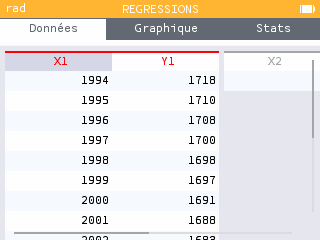
\includegraphics[height=3cm]{./graphics/pl-doc-stats_a}~~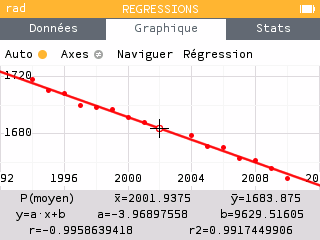
\includegraphics[height=3cm]{./graphics/pl-doc-stats_b}~~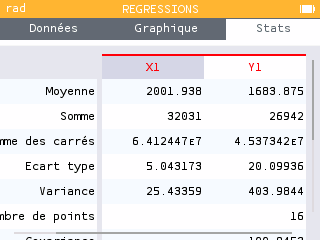
\includegraphics[height=3cm]{./graphics/pl-doc-stats_c}~~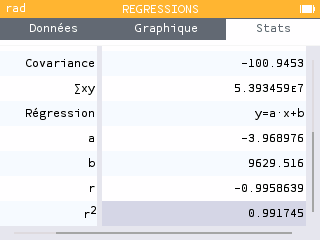
\includegraphics[height=3cm]{./graphics/pl-doc-stats_c2}\hfill~
\end{codeinfo}

\begin{codeinfo}
Les \textsf{macros} qui contiennent les paramètres de la régression sont donc réutilisables, en tant que nombres réels, donc exploitables par \ctex{siunitx} et \ctex{xfp} pour affichage \textit{fin} ! Ci-dessous un exemple permettant de visualiser tout cela.
\end{codeinfo}

\begin{codetex}[listing only]
%les espaces verticaux n'ont pas été écrits ici
\def\LstX{0,1,3,4,5,6}
\def\LstY{-35,-37.4,-37.7,-39.9,-39,-39.6}
%on lance les calculs et on change le nom des "macros-résultats"
\PLreglin[nomcoeffa=TESTa,nomcoeffb=TESTb,nomcoeffr=TESTr,nomcoeffrd=TESTrd,%
          nomxmin=TESTmin,nomxmax=TESTmax]{\LstX}{\LstY}
%commandes complémentaires
\DeclareDocumentCommand\arrond{ s O{3} m }{% * pour afficher signe / opt = précision / argument = nb
	\IfBooleanTF{#1}{\num[print-implicit-plus]{\fpeval{round(#3,#2)}}}{\num{\fpeval{round(#3,#2)}}}
}
%paramètres
Les valeurs extr. de X sont \TESTmin{} et \TESTmax. Une éq. est $y=\arrond[3]{\TESTa}x \arrond*[3]{\TESTb}$.
Le coeff. de corrélation est $r=\arrond[4]{\TESTr}$, et son carré est $r^2=\arrond[4]{\TESTrd}$.
\end{codetex}

\begin{codesortie}
\def\LstX{0,1,3,4,5,6}\def\LstY{-35,-37.4,-37.7,-39.9,-39,-39.6}
\PLreglin[nomcoeffa=TESTa,nomcoeffb=TESTb,nomcoeffr=TESTr,nomcoeffrd=TESTrd,nomxmin=TESTmin,nomxmax=TESTmax]{\LstX}{\LstY}
\DeclareDocumentCommand\arrond{ s O{3} m }{
	\IfBooleanTF{#1}{\num[print-implicit-plus]{\fpeval{ceil(#3,#2)}}}
		{\num{\fpeval{round(#3,#2)}}}
}

Les valeurs extrêmes de X sont \TESTmin{} et \TESTmax. Une équation de la droite de régression de $y$ en $x$ est $y=\arrond[3]{\TESTa}x \arrond*[3]{\TESTb}$.

\smallskip

Le coefficient de corrélation linéaire est $r=\arrond[4]{\TESTr}$, et son carré est $r^2=\arrond[4]{\TESTrd}$.
\end{codesortie}

\begin{codeinfo}
\hfill~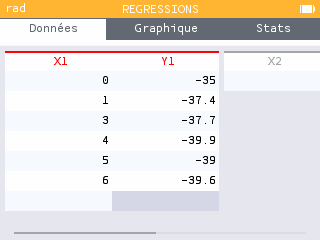
\includegraphics[height=3cm]{./graphics/pl-doc-stats_d}~~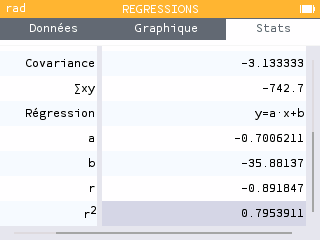
\includegraphics[height=3cm]{./graphics/pl-doc-stats_e}\hfill~
\end{codeinfo}

\subsection{Intégration dans un environnement \TikZ}

\begin{codeinfo}
La commande étant \og autonome \fg{}, elle va pouvoir être intégrée dans des environnements graphiques pour permettre un tracé \textit{facile} de la droite de régression.
\end{codeinfo}

\begin{codetex}[listing only]
\begin{tikzpicture}
	\begin{axis}[<options des axes, non présentées ici...>]
		\addplot[teal, only marks] table{
			X Y
			1994 1718 1995 1710 1996 1708 1997 1700 1998 1698 1999 1697 2000 1691 2001 1688
			2002 1683 2004 1679 2005 1671 2006 1670 2007 1663 2008 1661 2009 1656 2010 1649
		};
		\def\LLX{1994,1995,1996,1997,1998,1999,2000,2001,2002,2004,2005,2006,2007,2008,2009,2010}
		\def\LLY{1718,1710,1708,1700,1698,1697,1691,1688,1683,1679,1671,1670,1663,1661,1656,1649}
		\PLreglin{\LLX}{\LLY}
		\addplot [thick,orange,domain=\LXmin:\LXmax,samples=2]{\COEFFa*x+\COEFFb};
		\addlegendentry{$y = \fpeval{round(\COEFFa,3)}\,x + \fpeval{round(\COEFFb,3)}$};
		\addlegendentry{$R^2=\fpeval{round(\COEFFrd,5)}$};
	\end{axis}
\end{tikzpicture}
\end{codetex}

\begin{codesortie}
\begin{tikzpicture}
	\begin{axis}[
		/pgf/number format/.cd,
		use comma,
		xmin = 1992, xmax = 2012,
		ymin = 1640, ymax = 1730,
		width = 0.7\textwidth,
		height = 0.35\textwidth,
		xtick distance = 2,
		ytick distance = 10,
		grid = both,
		minor tick num = 1,
		major grid style = {lightgray},
		minor grid style = {lightgray!25},
		xlabel = {\small Année ($x$)},
		ylabel = {\small Altitude du glacier (en m) ($y$)},
		x tick label style={/pgf/number format/.cd, set thousands separator={}},
		y tick label style={/pgf/number format/.cd, set thousands separator={}},
		legend cell align = {left},
		legend pos = north east
		]
		\addplot[teal, only marks] table{
			X Y
			1994 1718
			1995 1710
			1996 1708
			1997 1700
			1998 1698
			1999 1697
			2000 1691
			2001 1688
			2002 1683
			2004 1679
			2005 1671
			2006 1670
			2007 1663
			2008 1661
			2009 1656
			2010 1649
		};
		\def\LLX{1994,1995,1996,1997,1998,1999,2000,2001,2002,2004,2005,2006,2007,2008,2009,2010}
		\def\LLY{1718,1710,1708,1700,1698,1697,1691,1688,1683,1679,1671,1670,1663,1661,1656,1649}
		\PLreglin{\LLX}{\LLY}
		\addplot [thick,orange,domain=\LXmin:\LXmax,samples=2]{\COEFFa*x+\COEFFb};
		\addlegendentry{$y = \fpeval{round(\COEFFa,3)}\,x + \fpeval{round(\COEFFb,3)}$};
		\addlegendentry{$R^2=\fpeval{round(\COEFFrd,5)}$};
	\end{axis}
\end{tikzpicture}
\end{codesortie}

\begin{codeinfo}
Il existe également une commande auxiliaire, \ctex{PLreglinpts} pour afficher le nuage de points avec quelques options, dans un environnement \TikZ{} classique (sans \textsf{pgfplot})\ldots
\end{codeinfo}

\begin{codetex}[listing only]
...
\begin{tikzpicture}[<options>]
	...
	\PLreglinpts[<clés>]{<listeX>}{<listeY>}
	...
\end{tikzpicture}
\end{codetex}

\begin{codecles}
Quelques \Cle{Clés} sont disponibles pour cette commande, essentiellement pour la mise en forme du nuage :

\begin{itemize}
	\item la clé \Cle{couleur} pour la couleur des points du nuage ;\hfill{}défaut \Cle{teal}
	\item la clé \Cle{taille} pour la taille des points (type \textit{cercle}) ;\hfill{}défaut \Cle{2pt}
	\item la clé \Cle{Ox} pour spécifier la valeur initiale Ox (si changement d'origine) ;\hfill{}défaut \Cle{0}
	\item la clé \Cle{Oy} pour spécifier la valeur initiale Oy (si changement d'origine).\hfill{}défaut \Cle{0}
\end{itemize}
\end{codecles}

\begin{codetex}[listing only]
\begin{tikzpicture}[x=0.5cm,y=0.05cm]
	\draw[xstep=1,ystep=5,lightgray!50,very thin] (0,0) grid (20,100);
	\draw[xstep=2,ystep=10,lightgray,thin] (0,0) grid (20,100);
	\draw[thick,->] (0,0)--(20,0) ;
	\draw[thick,->] (0,0)--(0,100) ;
	\foreach \x in {1992,1994,...,2010} \draw[thick] ({\x-1992},4pt)--({\x-1992},-4pt) node[below] {$\x$} ;
	\foreach \y in {1640,1650,...,1730} \draw[thick] (4pt,{\y-1640})--(-4pt,{\y-1640}) node[left] {$\y$} ;
	\def\LLX{1994,1995,1996,1997,1998,1999,2000,2001,2002,2004,2005,2006,2007,2008,2009,2010}
	\def\LLY{1718,1710,1708,1700,1698,1697,1691,1688,1683,1679,1671,1670,1663,1661,1656,1649}
	\def\Ox{1992}\def\Oy{1640}
	\PLreglin{\LLX}{\LLY}
	\PLreglinpts[Ox=1992,Oy=1640,couleur=blue,taille=3pt]{\LLX}{\LLY}
	\draw[orange,very thick,samples=2,domain=\LXmin:\LXmax] plot ({\x-\Ox},{\COEFFa*(\x)+\COEFFb-\Oy}) ;
	\matrix [draw,fill=white,below left] at (current bounding box.north east) {
		\node {$y = \fpeval{round(\COEFFa,3)}\,x + \fpeval{round(\COEFFb,3)}$} ; \\
		\node {$R^2=\fpeval{round(\COEFFrd,5)}$} ; \\
	};
\end{tikzpicture}
\end{codetex}

\begin{codesortie}
\begin{tikzpicture}[x=0.5cm,y=0.05cm]
	\draw[xstep=1,ystep=5,lightgray!50,very thin] (0,0) grid (20,100);
	\draw[xstep=2,ystep=10,lightgray,thin] (0,0) grid (20,100);
	\draw[thick,->] (0,0)--(20,0) ;
	\draw[thick,->] (0,0)--(0,100) ;
	\foreach \x in {1992,1994,...,2010} \draw[thick] ({\x-1992},4pt)--({\x-1992},-4pt) node[below] {$\x$} ;
	\foreach \y in {1640,1650,...,1730} \draw[thick] (4pt,{\y-1640})--(-4pt,{\y-1640}) node[left] {$\y$} ;
	\def\LLX{1994,1995,1996,1997,1998,1999,2000,2001,2002,2004,2005,2006,2007,2008,2009,2010}
	\def\LLY{1718,1710,1708,1700,1698,1697,1691,1688,1683,1679,1671,1670,1663,1661,1656,1649}
	\def\Ox{1992}\def\Oy{1640}
	\PLreglin{\LLX}{\LLY}
	\PLreglinpts[Ox=1992,Oy=1640,couleur=blue,taille=3pt]{\LLX}{\LLY}
	\draw[orange,very thick,samples=2,domain=\LXmin:\LXmax] plot ({\x-\Ox},{\COEFFa*(\x)+\COEFFb-\Oy}) ;
	\matrix [draw,fill=white,below left] at (current bounding box.north east) {
		\node {$y = \fpeval{round(\COEFFa,3)}\,x + \fpeval{round(\COEFFb,3)}$} ; \\
		\node {$R^2=\fpeval{round(\COEFFrd,5)}$} ; \\
	};
\end{tikzpicture}
\end{codesortie}

\newpage

\section{Statistiques à deux variables}\label{statsdeuxvars}

\subsection{Idées}

\begin{codeidee}
L'idée est de \textit{prolonger} le paragraphe précédent pour proposer un environnement \TikZ{} adapté à des situations venant de statistiques à deux variables.

\smallskip

Un des soucis pour ces situations est le fait que le repère dans lequel on travaille n'a pas forcément pour origine $(0\,;\,0)$.

De ce fait - pour éviter des erreurs de \ctex{dimension too large} liées à \TikZ{} - il faut \textit{décaler les axes} pour se ramener à une origine en $O$.

\smallskip

Le code, intimement lié à un environnement \ctex{tikzpicture}, va donc :

\begin{itemize}
	\item préciser les informations utiles comme \ctex{xmin}, \ctex{xmax}, \ctex{Ox}, \ctex{xgrille}, etc
	\item proposer des commandes (sans se soucier des \textit{translations} !) pour :
	\begin{itemize}
		\item tracer une grille (principale et/ou secondaire) ;
		\item tracer les axes (avec légendes éventuelles) et éventuellement les graduer ;
	\end{itemize}
\end{itemize}

En utilisant les commandes de \textsf{régression linéaire} du paragraphe précédent, il sera de plus possible (sans calculs !) de :

\begin{itemize}
	\item représenter le nuage de points ;
	\item placer le point moyen ;
	\item tracer la droite d'ajustement (obtenue par \ctex{ProfLycee}) ou une autre courbe.
\end{itemize}
\end{codeidee}

\begin{codeinfo}
Le package \ctex{pgfplots} peut être utilisé pour traiter ce genre de situation, mais ne l'utilisant pas, j'ai préféré préparer des \textsf{macros} permettant de s'affranchir de ce package (est-ce pertinent, ça c'est une autre question\ldots).
\end{codeinfo}

\begin{codetex}[listing only]
%Listes et calculs
\def\LLX{1994,1995,1996,1997,1998,1999,2000,2001,2002,2004,2005,2006,2007,2008,2009,2010}
\def\LLY{1718,1710,1708,1700,1698,1697,1691,1688,1683,1679,1671,1670,1663,1661,1656,1649}
\PLreglin{\LLX}{\LLY}
\end{codetex}

\begin{codetex}[listing only]
%tracé (simple), les options seront présentées juste après
\begin{tikzpicture}%
	[x=0.5cm,y=0.1cm,                                                 %unités
	Ox=1992,xmin=1992,xmax=2012,xgrille=2,xgrilles=1,                 %axe Ox
	Oy=1640,ymin=1640,ymax=1730,ygrille=10,ygrilles=5]                %axe Oy
	\PLgrilletikz \PLaxestikz                                         %grilles et axes
	\PLaxextikz[annee]{1992,1994,...,2010}                            %axeOx
	\PLaxeytikz{1640,1650,...,1720}                                   %axeOy
	\PLnuagepts{\LLX}{\LLY}                                           %nuage
	\PLcourbe[line width=1.25pt,ForestGreen,samples=2]%
		{\COEFFa*\x+\COEFFb}{\LXmin:\LXmax}                             %droite de régression
	\PLnuageptmoy                                                     %point moyen
\end{tikzpicture}
\end{codetex}

\begin{codetex}[listing only]
%tracé avec options fenêtre par défaut
\begin{tikzpicture}%
	[....]                                                            %paramètres
	\PLfenetresimple<annee>{1992,1994,...,2010}{1640,1650,...,1720}   %fenêtre "simple"
	\PLnuagepts{\LLX}{\LLY}                                           %nuage
	\PLcourbe[line width=1.25pt,ForestGreen,samples=2]%
	{\COEFFa*\x+\COEFFb}{\LXmin:\LXmax}                               %droite de régression
	\PLnuageptmoy                                                     %point moyen
\end{tikzpicture}
\end{codetex}

\begin{codesortie}
\def\LLX{1994,1995,1996,1997,1998,1999,2000,2001,2002,2004,2005,2006,2007,2008,2009,2010}
\def\LLY{1718,1710,1708,1700,1698,1697,1691,1688,1683,1679,1671,1670,1663,1661,1656,1649}
\PLreglin{\LLX}{\LLY}

\begin{tikzpicture}[x=0.5cm,y=0.1cm,Ox=1992,xmin=1992,xmax=2012,xgrille=2,xgrilles=1,Oy=1640,ymin=1640,ymax=1730,ygrille=10,ygrilles=5]
	\PLgrilletikz \PLaxestikz
	\PLaxextikz[annee]{1992,1994,...,2010}
	\PLaxeytikz{1640,1650,...,1720}
	\PLnuagepts{\LLX}{\LLY}
	\PLcourbe[line width=1.25pt,ForestGreen,samples=2]{\COEFFa*\x+\COEFFb}{\LXmin:\LXmax}
	\PLnuageptmoy
\end{tikzpicture}
\end{codesortie}

\subsection{Commandes, clés et options}

\begin{codeinfo}
Les \Cle{paramètres} nécessaires à la bonne utilisation des commandes suivantes sont à déclarer directement dans l'environnement \ctex{tikzpicture}, seules versions \og x \fg{}  sont présentées ici:

\begin{itemize}
	\item \Cle{xmin}, stockée dans \ctex{\textbackslash{}xmin} ;\hfill{}défaut \Cle{-3}
	\item \Cle{xmax}, stockée dans \ctex{\textbackslash{}xmax} ;\hfill{}défaut \Cle{3}
	\item \Cle{Ox}, stockée dans \ctex{\textbackslash{}axexOx}, origine de l'axe $(Ox)$ ;\hfill{}défaut \Cle{0}
	\item \Cle{xgrille}, stockée dans \ctex{\textbackslash{}xgrille}, graduation principale ;\hfill{}défaut \Cle{1}
	\item \Cle{xgrilles}, stockée dans \ctex{\textbackslash{}xgrilles}, graduation secondaire.\hfill{}défaut \Cle{0.5}
\end{itemize}

La fenêtre d'affichage (de sortie) sera donc \textit{portée} par le rectangle de coins $(xmin\,;\,ymin)$ et $(xmax\,;\,ymax)$ ; ce qui correspond en fait à la fenêtre \TikZ{} \textit{portée} par le rectangle de coins $(xmin-Ox\,;\,ymin-Oy)$ et $(xmax-Ox\,;\,ymax-Oy)$.

\smallskip

Les commandes ont -- pour certaines -- pas mal de \Cle{clés} pour des réglages fins, mais dans la majorité des cas elles ne sont pas forcément \textit{utiles}.
\end{codeinfo}

\begin{codeinfo}
Pour illustrer les commandes et options de ce paragraphe, la base sera le graphique présenté précédemment.
\end{codeinfo}

\begin{codetex}[listing only]
%...code tikz
	\PLgrilletikz[<options>][<options grille ppale>][<options grille second.>]
\end{codetex}

\begin{codecles}
Cette commande permet de tracer une grille principale et/ou une grille secondaire :

\begin{itemize}
	\item les premières \Cle{clés} sont les booléens \Cle{affp} et \Cle{affs} qui affichent ou non les grilles ;\hfill~défaut \Cle{true}
	\item les options des grilles sont en \TikZ. \hfill~défaut \Cle{thin,lightgray} et \Cle{very thin,lightgray}
\end{itemize}
\end{codecles}

\begin{codetex}[listing only]
\begin{tikzpicture}%
	[x=0.35cm,y=0.07cm,%
	Ox=1992,xmin=1992,xmax=2012,xgrille=2,xgrilles=1,%
	Oy=1640,ymin=1640,ymax=1730,ygrille=10,ygrilles=5]
	\PLgrilletikz
\end{tikzpicture}
~~
\begin{tikzpicture}%
	[x=0.35cm,y=0.07cm,%
	Ox=1992,xmin=1992,xmax=2012,xgrille=2,xgrilles=1,%
	Oy=1640,ymin=1640,ymax=1730,ygrille=10,ygrilles=5]
	\PLgrilletikz[affp=false][][orange,densely dotted]
\end{tikzpicture}
\end{codetex}

\begin{codesortie}
\hfill~
\begin{tikzpicture}%
	[x=0.35cm,y=0.07cm,%
	Ox=1992,xmin=1992,xmax=2012,xgrille=2,xgrilles=1,%
	Oy=1640,ymin=1640,ymax=1730,ygrille=10,ygrilles=5]
	\PLgrilletikz
\end{tikzpicture}
~~
\begin{tikzpicture}%
	[x=0.35cm,y=0.07cm,%
	Ox=1992,xmin=1992,xmax=2012,xgrille=2,xgrilles=1,%
	Oy=1640,ymin=1640,ymax=1730,ygrille=10,ygrilles=5]
	\PLgrilletikz[affp=false][][orange,densely dotted]
\end{tikzpicture}
\hfill~
\end{codesortie}

\begin{codetex}[listing only]
%...code tikz
	\PLaxestikz[<options>]
\end{codetex}

\begin{codecles}
Cette commande permet de tracer les axes, avec des \Cle{clés} :

\begin{itemize}
	\item \Cle{epaisseur} qui est l'épaisseur des traits ; \hfill~défaut \Cle{1.25pt}
	\item \Cle{police} qui est le style des labels des axes  ; \hfill~défaut \Cle{\textbackslash{}normalsize\textbackslash{}normalfont}
	\item \Cle{labelx} qui est le label de l'axe $(Ox)$ ; \hfill~défaut \Cle{\${}x\$}
	\item \Cle{labely} qui est le label de l'axe $(Oy)$ ; \hfill~défaut \Cle{\${}y\$}
	\item \Cle{afflabel} qui est le code pour préciser quels labels afficher, entre \Cle{x}, \Cle{y} ou \Cle{xy} ; \hfill~défaut \Cle{vide}
	\item \Cle{poslabelx} pour la position du label de $(Ox)$ en bout d'axe ; \hfill~défaut \Cle{right}
	\item \Cle{poslabely} pour la position du label de $(Oy)$ en bout d'axe ; \hfill~défaut \Cle{above}
	\item \Cle{echellefleche} qui est l'échelle de la flèche des axes ; \hfill~défaut \Cle{1}
	\item \Cle{typefleche} qui est le type de la flèche des axes.\hfill~défaut \Cle{>}
\end{itemize}
\end{codecles}

\begin{codetex}[listing only]
%code tikz
	\PLaxestikz

%code tikz
	\PLaxestikz%
		[afflabel=xy,labelx={Année},labely={Altitude},%
		poslabelx={below right},poslabely={above left}%
		police=\small\sffamily]
\end{codetex}

\begin{codesortie}
\hfill~
\begin{tikzpicture}%
	[x=0.35cm,y=0.07cm,%
	Ox=1992,xmin=1992,xmax=2012,xgrille=2,xgrilles=1,%
	Oy=1640,ymin=1640,ymax=1730,ygrille=10,ygrilles=5]
	\PLaxestikz
\end{tikzpicture}
~~
\begin{tikzpicture}%
	[x=0.35cm,y=0.07cm,%
	Ox=1992,xmin=1992,xmax=2012,xgrille=2,xgrilles=1,%
	Oy=1640,ymin=1640,ymax=1730,ygrille=10,ygrilles=5]
	\PLaxestikz%
		[afflabel=xy,labelx={Année},labely={Altitude},%
		poslabelx={below right},poslabely={above left},%
		police=\small\sffamily]
\end{tikzpicture}
\hfill~
\end{codesortie}

%les axes

\begin{codetex}[listing only]
%...code tikz
	\PLaxextikz[<options>]{valeurs}
	\PLaxeytikz[<options>]{valeurs}
\end{codetex}

\begin{codecles}
Ces commande permet de tracer les graduations des axes, avec des \Cle{clés} identiques pour les deux directions :

\begin{itemize}
	\item \Cle{epaisseur} qui est l'épaisseur des graduations ; \hfill~défaut \Cle{1.25pt}
	\item \Cle{police} qui est le style des labels des graduations ; \hfill~défaut \Cle{\textbackslash{}normalsize\textbackslash{}normalfont}
	\item \Cle{posgrad} qui est la position des graduations par rapport à l'axe ; \hfill~défaut \Cle{below} et \Cle{left}
	\item \Cle{hautgrad} qui est la position des graduations (sous la forme \Cle{lgt} ou \Cle{lgta/lgtb}) ; \hfill~défaut \Cle{4pt}
	\item le booléen \Cle{affgrad} pour afficher les valeurs (formatés avec \ctex{num} donc dépendant de \ctex{sisetup}) des graduations  ; \hfill~défaut \Cle{true}
	\item le booléen \Cle{afforigine} pour afficher la graduation de l'origine ; \hfill~défaut \Cle{true}
	\item le booléen \Cle{annee} qui permet de ne pas formater les valeurs des graduations (type \textsf{année}). \hfill~défaut \Cle{false}
\end{itemize}
\end{codecles}

\begin{codetex}[listing only]
%code tikz
	\PLaxextikz[police=\small]{1992,1994,...,2010}
	\PLaxeytikz{1640,1650,...,1720}
	
%code tikz
	\PLaxextikz[police=\small,annee,hautgrad=0pt/4pt]{1992,1994,...,2010}
	\PLaxeytikz[affgrad=false,hautgrad=6pt]{1640,1650,...,1720}

%des axes fictifs (en gris) sont rajoutés pour la lisibilité du code de sortie
\end{codetex}

\begin{codesortie}
\hfill~
\begin{tikzpicture}%
	[x=0.35cm,y=0.07cm,%
	Ox=1992,xmin=1992,xmax=2012,xgrille=2,xgrilles=1,%
	Oy=1640,ymin=1640,ymax=1730,ygrille=10,ygrilles=5]
	\draw[gray,line width=1.25pt,->] ({\xmin-\axexOx},0) -- ({\xmax-\axexOx},0) ;
	\draw[gray,line width=1.25pt,->] (0,{\ymin-\axeyOy}) -- (0,{\ymax-\axeyOy}) ;
	\PLaxextikz[police=\small]{1992,1994,...,2010}
	\PLaxeytikz{1640,1650,...,1720}
\end{tikzpicture}
~~
\begin{tikzpicture}%
	[x=0.35cm,y=0.07cm,%
	Ox=1992,xmin=1992,xmax=2012,xgrille=2,xgrilles=1,%
	Oy=1640,ymin=1640,ymax=1730,ygrille=10,ygrilles=5]
	\draw[gray,line width=1.25pt,->] ({\xmin-\axexOx},0) -- ({\xmax-\axexOx},0) ;
	\draw[gray,line width=1.25pt,->] (0,{\ymin-\axeyOy}) -- (0,{\ymax-\axeyOy}) ;
	\PLaxextikz[police=\small,annee,hautgrad=0pt/4pt]{1992,1994,...,2010}
	\PLaxeytikz[affgrad=false,hautgrad=6pt]{1640,1650,...,1720}
\end{tikzpicture}
\hfill~
\end{codesortie}

\subsection{Commandes annexes}

\begin{codeinfo}
Il existe, de manière marginale, quelques commandes complémentaires qui ne seront pas trop détaillées mais qui sont présentes dans l'introduction :

\begin{itemize}
	\item \ctex{PLfenetre} qui restreint les tracés à la fenêtre (utile pour des courbes qui \textit{débordent}) ;
	\item \ctex{PLfenetresimple} qui permet d'automatiser le tracé des grilles/axes/graduations dans leurs versions par défaut, avec peu de paramétrages ;
	\item \ctex{PLorigine} pour rajouter le libellé de l'origine si non affiché par les axes.
\end{itemize}
\end{codeinfo}

\begin{codetex}[listing only]
%code tikz
	\PLfenetre                %on restreint les tracés
	\PLfenetresimple<options axe Ox>{liste abscisses}<options axe Oy>{liste ordonnées}
\end{codetex}

%%l'origine
%
%\begin{codetex}[listing only]
%%...code tikz
%	\PLorigine[<options>]
%\end{codetex}

\subsection{Interactions avec PLreglin}

\begin{codetex}[listing only]
%...code tikz
	\PLnuagepts[<options>]{listeX}{listeY}
\end{codetex}

\begin{codecles}
Cette commande, liée à la commande \ctex{PLreglin} permet de représenter le nuage de points associé aux deux listes, avec les \Cle{clés} suivantes :

\begin{itemize}
	\item \Cle{taille} qui est la taille des points du nuage ; \hfill~défaut \Cle{2pt}
	\item \Cle{style} parmi \Cle{o} (rond) ou \Cle{x} (croix) ou \Cle{+} (plus) ; \hfill~défaut \Cle{o}
	\item \Cle{couleur} qui est la couleur (éventuellement \Cle{couleurA/couleurB} pour les ronds). \hfill~défaut \Cle{blue}
\end{itemize}
\end{codecles}

\begin{codetex}[listing only]
\def\LLX{1994,1995,1996,1997,1998,1999,2000,2001,2002,2004,2005,2006,2007,2008,2009,2010}
\def\LLY{1718,1710,1708,1700,1698,1697,1691,1688,1683,1679,1671,1670,1663,1661,1656,1649}

\begin{tikzpicture}[...]
	\PLnuagepts[couleur=blue/red]{\LLX}{\LLY}
\end{tikzpicture}
~~
\begin{tikzpicture}[...]
	\PLnuagepts[couleur=ForestGreen,style=x,taille=6pt]{\LLX}{\LLY}
\end{tikzpicture}
\end{codetex}

\begin{codesortie}
\def\LLX{1994,1995,1996,1997,1998,1999,2000,2001,2002,2004,2005,2006,2007,2008,2009,2010}
\def\LLY{1718,1710,1708,1700,1698,1697,1691,1688,1683,1679,1671,1670,1663,1661,1656,1649}
\PLreglin{\LLX}{\LLY}

\begin{tikzpicture}[x=0.35cm,y=0.07cm,Ox=1992,xmin=1992,xmax=2012,xgrille=2,xgrilles=1,Oy=1640,ymin=1640,ymax=1730,ygrille=10,ygrilles=5]
	\PLgrilletikz \PLaxestikz
	\PLaxextikz[annee,police=\small]{1992,1994,...,2010}
	\PLaxeytikz{1640,1650,...,1720}
	\PLnuagepts[couleur=blue/red]{\LLX}{\LLY}
\end{tikzpicture}
~~
\begin{tikzpicture}[x=0.35cm,y=0.07cm,Ox=1992,xmin=1992,xmax=2012,xgrille=2,xgrilles=1,Oy=1640,ymin=1640,ymax=1730,ygrille=10,ygrilles=5]
	\PLgrilletikz \PLaxestikz
	\PLaxextikz[annee,police=\small]{1992,1994,...,2010}
	\PLaxeytikz{1640,1650,...,1720}
	\PLnuagepts[couleur=ForestGreen,style=x,taille=6pt]{\LLX}{\LLY}
\end{tikzpicture}
\end{codesortie}

%point moyen
\begin{codetex}[listing only]
%...code tikz
	\PLnuageptmoy[<options>]
\end{codetex}

\begin{codecles}
Cette commande permet de rajouter le point moyen du nuage, calculé par la commande \ctex{PLreglin}, avec les \Cle{clés} :

\begin{itemize}
	\item \Cle{police}, comme précédemment ; \hfill~défaut \Cle{\textbackslash{}normalsize\textbackslash{}normalfont} ;
	\item \Cle{taille}, taille du point moyen ; \hfill~défaut \Cle{4pt}
	\item \Cle{couleur}, couleur du point moyen ; \hfill~défaut \Cle{red}
	\item \Cle{style} parmi \Cle{o} (rond) ou \Cle{x} (croix) ou \Cle{+} (plus) ; \hfill~défaut \Cle{o}
	\item \Cle{xg}, abscisse du point moyen, récupérable via \ctex{PLRegLin} ; \hfill~défaut \Cle{\textbackslash{}LXmoy}
	\item \Cle{yg}, ordonnée du point moyen, récupérable via \ctex{PLRegLin} ; \hfill~défaut \Cle{\textbackslash{}LYmoy}
	\item \Cle{nom}, label du point moyen ; \hfill~défaut \Cle{G}
	\item \Cle{pos} qui est la position du label par rapport au point ; \hfill~défaut \Cle{above}
	\item \Cle{decal} qui est l'éloignement de la position du label par rapport au point ; \hfill~défaut \Cle{0pt}
	\item la booléen \Cle{affnom} qui affiche ou non le libellé.\hfill~défaut \Cle{true}
\end{itemize}
\end{codecles}

\begin{codetex}[listing only]
\def\LLX{1994,1995,1996,1997,1998,1999,2000,2001,2002,2004,2005,2006,2007,2008,2009,2010}
\def\LLY{1718,1710,1708,1700,1698,1697,1691,1688,1683,1679,1671,1670,1663,1661,1656,1649}
\PLreglin{\LLX}{\LLY}

\begin{tikzpicture}[...]
	\PLnuagepts[couleur=blue/red]{\LLX}{\LLY}
	\PLnuageptmoy
\end{tikzpicture}
~~
\begin{tikzpicture}[...]
	\PLnuagepts[couleur=ForestGreen,style=x,taille=6pt]{\LLX}{\LLY}
	\PLnuageptmoy[couleur=orange,taille=8pt,style=+,nom={$G_1$}]
\end{tikzpicture}
\end{codetex}

\begin{codesortie}
\def\LLX{1994,1995,1996,1997,1998,1999,2000,2001,2002,2004,2005,2006,2007,2008,2009,2010}
\def\LLY{1718,1710,1708,1700,1698,1697,1691,1688,1683,1679,1671,1670,1663,1661,1656,1649}
\PLreglin{\LLX}{\LLY}

\begin{tikzpicture}[x=0.35cm,y=0.07cm,Ox=1992,xmin=1992,xmax=2012,xgrille=2,xgrilles=1,Oy=1640,ymin=1640,ymax=1730,ygrille=10,ygrilles=5]
	\PLgrilletikz \PLaxestikz
	\PLaxextikz[annee,police=\small]{1992,1994,...,2010}
	\PLaxeytikz{1640,1650,...,1720}
	\PLnuagepts[couleur=blue/red]{\LLX}{\LLY}
	\PLnuageptmoy
\end{tikzpicture}
~~
\begin{tikzpicture}[x=0.35cm,y=0.07cm,Ox=1992,xmin=1992,xmax=2012,xgrille=2,xgrilles=1,Oy=1640,ymin=1640,ymax=1730,ygrille=10,ygrilles=5]
	\PLgrilletikz \PLaxestikz
	\PLaxextikz[annee,police=\small]{1992,1994,...,2010}
	\PLaxeytikz{1640,1650,...,1720}
	\PLnuagepts[couleur=ForestGreen,style=x,taille=6pt]{\LLX}{\LLY}
	\PLnuageptmoy[couleur=orange,taille=8pt,style=+,nom={$G_1$},pos=below]
\end{tikzpicture}
\end{codesortie}

%courbe
\begin{codetex}[listing only]
%...code tikz
	\PLcourbe[<options>]{formule}{domaine}
\end{codetex}

\begin{codecles}
Cette commande permet de rajouter une courbe sur le graphique (sans se soucier de la transformation de son expression) avec les arguments :

\begin{itemize}
	\item \Cle{optionnels} qui sont - en \TikZ{} - les paramètres du tracé ;
	\item le premier mandataire, est - en langage \TikZ{} - l'expression de la fonction à tracer, donc avec \ctex{\textbackslash{}x} comme variable ;
	\item le second mandataire est le domaine du tracé , sous la forme \ctex{valxmin:valxmax}.
\end{itemize}
\end{codecles}

\begin{codeinfo}
L'idée principale est de récupérer les variables de la régression linéaire pour tracer la droite d'ajustement \textit{à moindres frais} !
\end{codeinfo}

\begin{codeinfo}
	Toute courbe peut être tracée sur ce principe, par contre il faudra saisir la fonction \textit{à la main}.
\end{codeinfo}

\begin{codetex}[listing only]
\def\LLX{1994,1995,1996,1997,1998,1999,2000,2001,2002,2004,2005,2006,2007,2008,2009,2010}
\def\LLY{1718,1710,1708,1700,1698,1697,1691,1688,1683,1679,1671,1670,1663,1661,1656,1649}
\PLreglin{\LLX}{\LLY}

\begin{tikzpicture}[...]
	\PLnuagepts[couleur=blue/red]{\LLX}{\LLY} \PLnuageptmoy
	\PLcourbe[line width=1.25pt,ForestGreen,samples=2]{\COEFFa*\x+\COEFFb}{\xmin:\xmax}
\end{tikzpicture}
\end{codetex}

\begin{codesortie}
\def\LLX{1994,1995,1996,1997,1998,1999,2000,2001,2002,2004,2005,2006,2007,2008,2009,2010}
\def\LLY{1718,1710,1708,1700,1698,1697,1691,1688,1683,1679,1671,1670,1663,1661,1656,1649}
\PLreglin{\LLX}{\LLY}

\begin{tikzpicture}[x=0.35cm,y=0.07cm,Ox=1992,xmin=1992,xmax=2012,xgrille=2,xgrilles=1,Oy=1640,ymin=1640,ymax=1730,ygrille=10,ygrilles=5]
	\PLgrilletikz \PLaxestikz
	\PLaxextikz[annee,police=\small]{1992,1994,...,2010}
	\PLaxeytikz{1640,1650,...,1720}
	\PLnuagepts[couleur=blue/red]{\LLX}{\LLY} \PLnuageptmoy
	\PLcourbe[line width=1.25pt,ForestGreen,samples=2]{\COEFFa*\x+\COEFFb}{\xmin:\xmax}
\end{tikzpicture}
\end{codesortie}

\begin{codetex}[listing only]
\def\LLX{1994,1995,1996,1997,1998,1999,2000,2001,2002,2004,2005,2006,2007,2008,2009,2010}
\def\LLY{1718,1710,1708,1700,1698,1697,1691,1688,1683,1679,1671,1670,1663,1661,1656,1649}

\begin{tikzpicture}[...]
	\PLnuagepts[couleur=blue/red]{\LLX}{\LLY} \PLfenetre %on fixe la fenêtre
	\PLcourbe[line width=1.25pt,orange,samples=500]{-(\x-2000)*(\x-2000)+1700}{\xmin:\xmax}
\end{tikzpicture}
\end{codetex}

\begin{codesortie}
\def\LLX{1994,1995,1996,1997,1998,1999,2000,2001,2002,2004,2005,2006,2007,2008,2009,2010}
\def\LLY{1718,1710,1708,1700,1698,1697,1691,1688,1683,1679,1671,1670,1663,1661,1656,1649}

\begin{tikzpicture}[x=0.35cm,y=0.07cm,Ox=1992,xmin=1992,xmax=2012,xgrille=2,xgrilles=1,Oy=1640,ymin=1640,ymax=1730,ygrille=10,ygrilles=5]
	\PLgrilletikz \PLaxestikz
	\PLaxextikz[annee,police=\small]{1992,1994,...,2010}
	\PLaxeytikz{1640,1650,...,1720}
	\PLnuagepts[couleur=blue/red]{\LLX}{\LLY} \PLfenetre
	\PLcourbe[line width=1.25pt,orange,samples=500]{-(\x-2000)*(\x-2000)+1700}{\xmin:\xmax}
\end{tikzpicture}
\end{codesortie}

\newpage

\section{Boîtes à moustaches}\label{boiteamoustaches}

\subsection{Introduction}

\begin{codeidee}
L'idée est de proposer une commande, à intégrer dans un environnement \TikZ, pour tracer une boîte à moustaches grâce aux paramètres, saisis par l'utilisateur.

\smallskip

Le code ne calcule pas les paramètres, il ne fait \textit{que} tracer la boîte à moustaches !
\end{codeidee}

\begin{codetex}[]
\begin{tikzpicture}
	\PLboitemoust[parametres={10/15/17/19/20}]
\end{tikzpicture}
\end{codetex}

\begin{codeinfo}
Étant donnée que la commande est intégrée dans un environnement \TikZ, les unités peuvent/doivent donc être précisées, \textit{comme d'habitude}, si besoin.
\end{codeinfo}

\subsection{Clés et options}

\begin{codecles}
Quelques \Cle{clés} sont disponibles pour cette commande :

\begin{itemize}
	\item la clé \Cle{parametres} qui sont sous la forme \Cle{Min/Q1/Med/Q3/Max} ;
	\item la clé \Cle{couleur} qui est la couleur de la boîte ; \hfill~défaut \Cle{black}
	\item la clé \Cle{elevation} qui est la position verticale (ordonnée des moustaches) de la boîte ; \hfill~défaut \Cle{1.5}
	\item la clé \Cle{hauteur} qui est la hauteur de la boîte ; \hfill~défaut \Cle{1}
	\item la clé \Cle{moyenne} qui est la moyenne (optionnelle) de la série ;
	\item la clé \Cle{epaisseur} qui est l'épaisseur des traits de la boîte ; \hfill~défaut \Cle{thick}
	\item la clé \Cle{remplir} qui est la couleur de remplissage de la boîte ; \hfill~défaut \Cle{white}
	\item le booléen \Cle{affmoyenne} qui permet d'afficher ou non la moyenne (sous forme d'un point) ; \hfill~défaut \Cle{false}
	\item le booléen \Cle{pointilles} qui permet d'afficher des pointillés au niveau des paramètres ; \hfill~défaut \Cle{false}
	\item le booléen \Cle{valeurs} qui permet d'afficher les valeurs des paramètres au niveau des abscisses.\hfill~défaut \Cle{false}
\end{itemize}
\end{codecles}

\begin{codetex}[]
\begin{tikzpicture}
	\PLboitemoust[epaisseur=very thick,parametres={10/15/17/19/20},moyenne=18.5,couleur=blue,affmoyenne,%
	pointilles,valeurs,hauteur=2.25,elevation=2.75]
\end{tikzpicture}
\end{codetex}

\begin{codetex}[listing only]
%une grille a été rajoutée pour visualiser la "position verticale"
\begin{center}
	\begin{tikzpicture}[x=0.1cm]
		\PLboitemoust[epaisseur=ultra thick,parametres={100/150/170/190/200},couleur=blue]
		\PLboitemoust[epaisseur=thin,elevation=2.5,parametres={80/100/110/120/150},couleur=red]
		\PLboitemoust[elevation=4,parametres={100/140/145/160/210},couleur=ForestGreen,remplir=ForestGreen!25]
\end{tikzpicture}
\end{center}
\end{codetex}

\begin{codesortie}
\begin{center}
	\begin{tikzpicture}[x=0.1cm]
		\draw[xstep=10,ystep=0.5,very thin,lightgray] (80,0) grid (210,4.5) ;
		\foreach \x in {80,90,...,210} \draw[very thin,lightgray] (\x,3pt)--(\x,-3pt) node[below] {\num{\x}} ;
		\foreach \y in {0,0.5,...,4.5} \draw[very thin,lightgray] ($(210,\y)+(-3pt,0)$)--($(210,\y)+(3pt,0)$) node[right] {\num{\y}} ;
		\PLboitemoust[epaisseur=ultra thick,parametres={100/150/170/190/200},couleur=blue]
		\PLboitemoust[epaisseur=thin,elevation=2.5,parametres={80/100/110/120/150},couleur=red]
		\PLboitemoust[elevation=4,parametres={100/140/145/160/210},couleur=ForestGreen,remplir=ForestGreen!25]
	\end{tikzpicture}
\end{center}
\end{codesortie}

\subsection{Commande pour placer un axe horizontal}

\begin{codeidee}
L'idée est de proposer, en parallèle de la commande précédente, une commande pour tracer un axe horizontal \og sous \fg{} les éventuelles boîtes à moustaches.
\end{codeidee}

\begin{codetex}[]
\begin{tikzpicture}
	\PLboitemoustaxe[min=10,max=20]
	\PLboitemoust[parametres={10/15/17/19/20}]
\end{tikzpicture}
\end{codetex}

\begin{codetex}[]
\begin{tikzpicture}
	\PLboitemoustaxe[min=10,max=20,]
	\PLboitemoust[parametres={10/15/17/19/20},valeurs,pointilles]
\end{tikzpicture}
\end{codetex}

\begin{codecles}
Quelques \Cle{clés} sont disponibles pour cette commande :

\begin{itemize}
	\item la clé \Cle{min} qui est la valeur minimale de l'axe horizontal ;
	\item la clé \Cle{max} qui est la valeur minimale de l'axe horizontal ;
	\item la clé \Cle{elargir} qui est le pourcentage l'élargissement de l'axe ;\hfill~défaut \Cle{0.1}
	\item la clé \Cle{epaisseur} qui est l'épaisseur des traits de la boîte ; \hfill~défaut \Cle{thick}
	\item la clé \Cle{valeurs} qui est la liste (compréhensible en \TikZ) des valeurs à afficher.
\end{itemize}
\end{codecles}

\begin{codetex}[]
\begin{tikzpicture}
	\PLboitemoustaxe[min=8,max=21,affvaleurs,valeurs={8,9,...,21},elargir=0.02]
	\PLboitemoust[parametres={10/15/17/19/20},moyenne=18.5,couleur=blue]
	\PLboitemoust[elevation=2.5,parametres={8/10/11/12/15},couleur=red]
	\PLboitemoust[elevation=4,parametres={10/14/14.5/16/21},couleur=ForestGreen,remplir=ForestGreen!25]
\end{tikzpicture}
\end{codetex}

\begin{codeinfo}
Le placement des différentes boîtes n'est pas automatique, donc il faut penser à cela avant de se lancer dans le code.

Sachant que la hauteur par défaut est de 1, il est -- a priori -- intéressant de placer les boîtes à des \Cle{élévations} de \num{1} puis \num{2.5} puis \num{4} etc
\end{codeinfo}

\newpage

\part{Outils pour les probabilités}

\section{Calculs de probabilités}\label{calcprobas}

\subsection{Introduction}

\begin{codeidee}
L'idée est de proposer des commandes permettant de calculer des probabilités avec des lois classiques :

\begin{itemize}
	\item binomiale ;
	\item normale ;
	\item exponentielle ;
	\item de Poisson ;
	\item géométrique ;
	\item hypergéométrique.
\end{itemize}
\end{codeidee}

\begin{codeinfo}
Les commandes sont de deux natures :

\begin{itemize}
	\item des commandes pour calculer, grâce au package \ctex{xintexpr} ;
	\item des commandes pour formater le résultat de \ctex{xintexpr}, grâce à \ctex{siunitx}.
\end{itemize}

De ce fait, les options de \ctex{siunitx} de l'utilisateur affecterons les formatages du résultat, la commande va \og forcer \fg{} les arrondis et l'écriture scientifique.
\end{codeinfo}

\subsection{Calculs \og simples \fg}

\begin{codetex}[listing only]
%loi binomiale B(n,p)
\calcPbinomP{n}{p}{k}             %P(X=k)
\calcPbinomC{n}{p}{a}{b}          %P(a<=X<=b)

%loi de Poisson P (l)
\calcPpoissP{l}{k}                %P(X=k)
\calcPpoissC{l}{a}{b}             %P(a<=X<=b)

%loi géométrique G (p)
\calcPgeomP{p}{k}                 %P(X=k)
\calcPgeomC{l}{a}{b}              %P(a<=X<=b)

%loi hypergéométrique H (N,n,m)
\calcPhypergeomP{N}{n}{m}{k}      %P(X=k)
\calcPhypergeomP{N}{n}{m}{a}{b}   %P(a<=X<=b)

%loi normale N(m,s)
\calcPnormC{m}{s}{a}{b}           %P(a<=X<=b)

%loi exponentielle E(l)
\calcPexpoC{l}{a}{b}              %P(a<=X<=b)
\end{codetex}

\begin{codecles}
Les probabilités calculables sont donc -- comme pour beaucoup de modèles de calculatrices -- les probabilités \textbf{P}onctuelles ($P(X=k)$) et \textbf{C}umulées ($P(a\leqslant X\leqslant b)$).

\smallskip

Pour les probabilités cumulées, on peut utiliser \ctex{*} comme borne ($a$ ou $b$), pour les probabilités du type $P(X\leqslant b)$ et $P(X \geqslant a)$.
\end{codecles}

\begin{codetex}[listing only]
% X -> B(5,0.4)
$P(X=3) \approx \calcPbinomP{5}{0.4}{3}$.
$P(X\leqslant1) \approx \calcPbinomC{5}{0.4}{*}{1}$.

% X -> B(100,0.02)
$P(X=10) \approx \calcPbinomP{100}{0.02}{10}$.
$P(15\leqslant X\leqslant25) \approx \calcPbinomC{100}{0.02}{15}{25}$.

% Y -> P(5)
$P(Y=3) \approx \calcPpoissP{5}{3}$.
$P(Y\geqslant2) \approx \calcPpoissC{5}{2}{*}$.

% T -> G(0.5)
$P(T=100) \approx \calcPgeomP{0.5}{3}$.
$P(T\leqslant5) \approx \calcPgeomC{0.5}{*}{5}$.

% W -> H(50,10,5)
$P(W=4) \approx \calcPhypergeomP{50}{10}{5}{4}$.
$P(1\leqslant W\leqslant3) \approx \calcPhypergeomP{50}{10}{5}{1}{3}$.
\end{codetex}

\begin{codesortie}[listing only]
$\bullet~~~~X \hookrightarrow \mathcal{B}(5\,;\,0,4)$ :\\
$P(X=3) \approx \calcPbinomP{5}{0.4}{3}$.\\
$P(X\leqslant1) \approx \calcPbinomC{5}{0.4}{*}{1}$.

\medskip

$\bullet~~~~X \hookrightarrow \mathcal{B}(100\,;\,0,02)$ :\\
$P(X=10) \approx \calcPbinomP{100}{0.02}{10}$.\\
$P(15\leqslant X\leqslant25) \approx \calcPbinomC{100}{0.02}{15}{25}$.

\medskip

$\bullet~~~~Y \hookrightarrow \mathcal{P}_5$ :\\
$P(Y=3) \approx \calcPpoissP{5}{3}$.\\
$P(Y\geqslant2) \approx \calcPpoissC{5}{2}{*}$.

\medskip

$\bullet~~~~T \hookrightarrow \mathcal{G}_{0,5}$ :\\
$P(T=3) \approx \calcPgeomP{0.5}{3}$.\\
$P(T\leqslant5) \approx \calcPgeomC{0.5}{*}{5}$.

\medskip

$\bullet~~~~W \hookrightarrow \mathcal{H}(50\,;\,10\,;\,5)$ :\\
$P(W=4) \approx \calcPhypergeomP{50}{10}{5}{4}$.\\
$P(1\leqslant W\leqslant3) \approx \calcPhypergeomC{50}{10}{5}{1}{3}$.
\end{codesortie}

\begin{codetex}[listing only]
% X -> N(0,1)
$P(X\leqslant1) \approx \calcPnormC{0}{1}{*}{1}$.
$P(-1,96\leqslant Z\leqslant1,96) \approx \calcPnormC{0}{1}{-1.96}{1.96}$.

% X -> N(550,30)
$P(Y\geqslant600) \approx \calcPnormC{550}{30}{600}{*}$.
$P(500\leqslant Y\leqslant600) \approx \calcPnormC{550}{30}{500}{600}$.

% Z -> E(0.001)
$P(Z\geqslant400) \approx \calcPexpoC{0.001}{400}{*}$.
$P(300\leqslant Z\leqslant750) \approx \calcPexpoC{0.001}{300}{750}$.
\end{codetex}

\begin{codesortie}
$\bullet~~~~X \hookrightarrow \mathcal{N}(0\,;\,1)$ :\\
$P(X\leqslant1) \approx \calcPnormC{0}{1}{*}{1}$.\\
$P(-1,96\leqslant Z\leqslant1,96) \approx \calcPnormC{0}{1}{-1.96}{1.96}$.

\medskip

$\bullet~~~~Y \hookrightarrow \mathcal{N}(550\,;\,30)$ :\\
$P(Y\geqslant600) \approx \calcPnormC{550}{30}{600}{*}$.\\
$P(500\leqslant Y\leqslant600) \approx \calcPnormC{550}{30}{500}{600}$.

\medskip

$\bullet~~~~Z \hookrightarrow \mathcal{E}_{0,001}$ :\\
$P(Z\geqslant400) \approx \calcPexpoC{0.001}{400}{*}$.\\
$P(300\leqslant Z\leqslant750) \approx \calcPexpoC{0.001}{300}{750}$.
\end{codesortie}

\subsection{Complément avec sortie \og formaté \fg}

\begin{codeidee}
L'idée est ensuite de formater le résultat obtenu par \ctex{xintexpr}, pour un affichage homogène.

\smallskip

L'utilisateur peut donc utiliser \og sa \fg{} méthode pour formater les résultats obtenus par \ctex{xintexpr} !
\end{codeidee}

\begin{codetex}[listing only]
%avec un formatage manuel
\num[exponent-mode=scientific]{\calcPbinomP{100}{0.02}{10}}
\end{codetex}

\begin{codesortie}
$\bullet~~~~X \hookrightarrow \mathcal{B}(100\,;\,0,02)$ :

$P(X=10) \approx \num[exponent-mode=scientific]{\calcPbinomP{100}{0.02}{10}}$.
\end{codesortie}

\begin{codeidee}
Le package \ctex{ProfLycee} propose -- en complément -- des commandes pour formater, grâce à \ctex{siunitx}, le résultat.

Les commandes sont dans ce cas préfixées par \ctex{num} au lieu de \ctex{calc} :

\begin{itemize}
	\item formatage sous forme décimale \textit{pure} : $0,00\ldots$ ;
	\item formatage sous forme scientifique : $n,\ldots\times10^{\ldots}$.
\end{itemize}
\end{codeidee}

\begin{codetex}[listing only]
%loi binomiale B(n,p)
\numPbinomP(*)[prec]{n}{p}{k}         %P(X=k)
\numPbinomC(*)[prec]{n}{p}{a}{b}      %P(a<=X<=b)

%loi de Poisson P (l)
\numPpoissP(*)[prec]{l}{k}            %P(X=k)
\numPpoissC(*)[prec]{l}{a}{b}         %P(a<=X<=b)

%loi géométrique G (p)
\numPgeomP{p}{k}                      %P(X=k)
\numPgeomC{l}{a}{b}                   %P(a<=X<=b)

%loi hypergéométrique H (N,n,m)
\numPhypergeomP{N}{n}{m}{k}           %P(X=k)
\numPhypergeomC{N}{n}{m}{a}{b}        %P(a<=X<=b)

%loi normale N(m,s)
\numPnormC(*)[prec]{m}{s}{a}{b}       %P(a<=X<=b)

%loi exponentielle E(l)
\numPexpoC(*)[prec]{l}{a}{b}          %P(a<=X<=b)
\end{codetex}

\begin{codecles}
Quelques précisions sur les commandes précédentes :

\begin{itemize}
	\item la version étoilée \Cle{*} des commandes formate le résultat en mode scientifique ;
	\item l'argument optionnel (par défaut \Cle{3}) correspond à quant à lui à l'arrondi.
\end{itemize}
\end{codecles}

\begin{codetex}[listing only]
% X -> N(550,30)
$P(Y\geqslant600) \approx \numPnormC[4]{550}{30}{600}{*}$.
$P(500\leqslant Y\leqslant600) \approx \numPnormC[4]{550}{30}{500}{600}$.
% X -> B(100,0.02)
$P(X=10) \approx \numPbinomP[7]{100}{0.02}{10} \approx \numPbinomP*[7]{100}{0.02}{10}$.
$P(15\leqslant X\leqslant25) \approx \numPbinomC[10]{100}{0.02}{15}{25} \approx \numPbinomC*[10]{100}{0.02}{15}{25}$.
% H -> H(50,10,5)
$P(W=4) \approx \numPhypergeomP[5]{50}{10}{5}{4}$.
$P(1\leqslant W\leqslant3) \approx \numPhypergeomC[4]{50}{10}{5}{1}{3}$.
% Z-> E(0,001)$ :
$P(Z\geqslant400) \approx \numPexpoC{0.001}{400}{*}$.
$P(300\leqslant Z\leqslant750) \approx \numPexpoC{0.001}{300}{750}$.
% T -> P(5)
$P(T=3) \approx \numPpoissP{5}{3}$.
$P(T\geqslant2) \approx \numPpoissC[4]{5}{2}{*}$.
\end{codetex}

\begin{codesortie}
$\bullet~~~~Y \hookrightarrow \mathcal{N}(550\,;\,30)$ :

$P(Y\geqslant600) \approx \numPnormC[4]{550}{30}{600}{*}$.

$P(500\leqslant Y\leqslant600) \approx \numPnormC[4]{550}{30}{500}{600}$.

\medskip

$\bullet~~~~X \hookrightarrow \mathcal{B}(100\,;\,0,02)$ :

$P(X=10) \approx \numPbinomP[7]{100}{0.02}{10} \approx \numPbinomP*[7]{100}{0.02}{10}$.

$P(15\leqslant X\leqslant25) \approx \numPbinomC[10]{100}{0.02}{15}{25} \approx \numPbinomC*[10]{100}{0.02}{15}{25}$.

\medskip

$\bullet~~~~W \hookrightarrow \mathcal{H}(50\,;\,10\,;\,5)$ :

$P(W=4) \approx \numPhypergeomP[5]{50}{10}{5}{4}$.

$P(1\leqslant W\leqslant3) \approx \numPhypergeomC[4]{50}{10}{5}{1}{3}$.

\medskip

$\bullet~~~~Z \hookrightarrow \mathcal{E}_{0,001}$ :

$P(Z\geqslant400) \approx \numPexpoC{0.001}{400}{*}$.

$P(300\leqslant Z\leqslant750) \approx \numPexpoC{0.001}{300}{750}$.

\medskip

$\bullet~~~~T \hookrightarrow \mathcal{P}_5$ :

$P(T=3) \approx \numPpoissP{5}{3}$.

$P(T\geqslant2) \approx \numPpoissC[4]{5}{2}{*}$.
\end{codesortie}

\begin{codeinfo}
\hfill~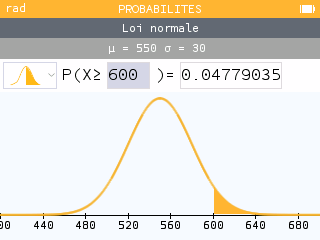
\includegraphics[height=3cm]{./graphics/pl-doc-probas_a}~~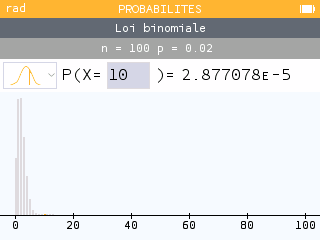
\includegraphics[height=3cm]{./graphics/pl-doc-probas_c}~~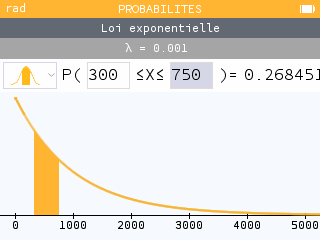
\includegraphics[height=3cm]{./graphics/pl-doc-probas_e}~~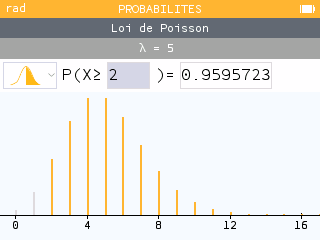
\includegraphics[height=3cm]{./graphics/pl-doc-probas_f}\hfill~
\end{codeinfo}

\newpage

\section{Arbres de probabilités \og classiques \fg}\label{arbresprobas}

\subsection{Introduction}

\begin{codeidee}
L'idée est de proposer des commandes pour créer des arbres de probabilités classiques (et homogènes), en \TikZ, de format :

\begin{itemize}
	\item $2\times2$ ou $2\times3$ ;
	\item $3\times2$ ou $3\times3$.
\end{itemize}

Les (deux) commandes sont donc liées à un environnement \ctex{tikzpicture}, et elles créent les nœuds de l'arbre, pour exploitation ultérieure éventuelle.
\end{codeidee}

\begin{codetex}[listing only]
%commande simple pour tracé de l'arbre
\PLarbre[<options>]{<donnees>}

%environnement pour tracé et exploitation éventuelle
\begin{PLenvarbre}[<options>]{<donnees>}
	<code tikz supplémentaire>
\end{PLenvarbre}
\end{codetex}

\subsection{Options et arguments}

\begin{codeinfo}
Les \Cle{donnees} seront à préciser sous forme \ctex{<sommet1>/<proba1>/<position1>,<sommet2>/<proba2>/<position2>,...} avec comme \og sens de lecture \fg{} de la gauche vers la droite puis du haut vers le bas (on balaye les \textit{sous-arbres}), avec comme possibilités :

\begin{itemize}
	\item une donnée \Cle{proba} peut être laissée vide ;
	\item une donnée \Cle{position} peut valoir \Cle{above} (au-dessus), \Cle{below} (en-dessous) ou être laissée \Cle{vide} (sur).
\end{itemize}
\end{codeinfo}

\begin{codecles}
Quelques \Cle{Clés} (communes) pour les deux commandes :

\begin{itemize}
	\item la clé \Cle{unite} pour préciser l'unité de l'environnement \TikZ{} ; \hfill~défaut \Cle{1cm}
	\item la clé \Cle{espniv} pour l'espace (H) entre les étages ; \hfill~défaut \Cle{3.25}
	\item la clé \Cle{espfeuille} pour l'espace (V) entre les feuilles ; \hfill~défaut \Cle{1}
	\item la clé \Cle{type} pour le format, parmi \Cle{2x2} ou \Cle{2x3} ou \Cle{3x2} ou  \Cle{3x3} ; \hfill~défaut \Cle{2x2}
	\item la clé \Cle{police} pour la police des nœuds ; \hfill~défaut \Cle{\textbackslash{}normalfont\textbackslash{}normalsize}
	\item la clé \Cle{policeprobas} pour la police des probas ; \hfill~défaut \Cle{\textbackslash{}normalfont\textbackslash{}small}
	\item le booléen \Cle{inclineprobas} pour incliner les probas ; \hfill~défaut \Cle{true}
	\item le booléen \Cle{fleche} pour afficher une flèche sur les branches ; \hfill~défaut \Cle{false}
	\item la clé \Cle{styletrait} pour les branches, en langage \TikZ{} ; \hfill~défaut \Cle{vide}
	\item la clé \Cle{eptrait} pour l'épaisseur des branches, en langage \TikZ{} ; \hfill~défaut \Cle{semithick}
\end{itemize}
\end{codecles}

\begin{codetex}[listing only]
\def\ArbreDeuxDeux{
	$A$/\num{0.5}/,
		$B$/\num{0.4}/,
		$\overline{B}$/.../,
	$\overline{A}$/.../,
		$B$/.../,
		$\overline{B}$/$\frac{1}{3}$/
}

\PLarbre{\ArbreDeuxDeux}

%des éléménts, en gris, ont été rajoutés pour illustrer certaines options
\end{codetex}

\begin{codesortie}
\begin{PLenvarbre}{$A$/\num{0.5}/,$B$/\num{0.4}/,$\overline{B}$/.../,$\overline{A}$/.../,$B$/.../,$\overline{B}$/$\frac{1}{3}$/}
	\draw[lightgray] (R) node[left,font=\ttfamily\small] {(R)} ;
	\draw[lightgray] (A11) node[below,font=\ttfamily\small] {(A11)} ;
	\draw[lightgray] (A12) node[below,font=\ttfamily\small] {(A12)} ;
	\draw[lightgray] (A21) node[below,font=\ttfamily\small] {(A21)} ;
	\draw[lightgray] (A22) node[below,font=\ttfamily\small] {(A22)} ;
	\draw[lightgray] (A23) node[below,font=\ttfamily\small] {(A23)} ;
	\draw[lightgray] (A24) node[below,font=\ttfamily\small] {(A24)} ;
	\draw[lightgray,<->] (0,-4) -- (3.25,-4) node[midway,below,font=\ttfamily\small] {espniv} ;
	\draw[lightgray,<->] (3.25,-4) -- (6.5,-4) node[midway,below,font=\ttfamily\small] {espniv} ;
	\draw[lightgray,<->] (7,0) -- (7,-1) node[midway,right,font=\ttfamily\small] {espfeuille} ;
	\draw[lightgray,<->] (7,-1) -- (7,-2) node[midway,right,font=\ttfamily\small] {espfeuille} ;
	\draw[lightgray,<->] (7,-2) -- (7,-3) node[midway,right,font=\ttfamily\small] {espfeuille} ;
\end{PLenvarbre}
\end{codesortie}

\begin{codeinfo}
Les nœuds crées par les commandes sont :

\begin{itemize}
	\item \ctex{R} pour la racine ;
	\item \ctex{A1x} pour les nœuds du 1\up{er} niveau (de haut en bas) ;
	\item  \ctex{A2x} pour les nœuds du 2\up{d} niveau (de haut en bas).
\end{itemize}
\end{codeinfo}

\subsection{Exemples complémentaires}

\begin{codetex}[listing only]
\def\ArbreTroisDeux{
	$A_1$/\num{0.5}/above,
		$B$/\num{0.4}/above,
		$\overline{B}$/.../below,
	$A_2$/.../above,
		$B$/.../above,
		$\overline{B}$/$\frac{1}{3}$/below,
	$A_3$/.../below,
		$B$/.../above,
		$\overline{B}$/$\frac{4}{15}$/below
}

\begin{PLenvarbre}[type=3x2,fleche,espniv=5,espfeuille=1.25]{\ArbreTroisDeux}
	\draw[ForestGreen,->] (A24)--($(A24)+(2.5,0)$) node[right,font=\sffamily] {code tikz rajouté} ;
\end{PLenvarbre}
\end{codetex}

\begin{codesortie}
\begin{PLenvarbre}[type=3x2,fleche,espniv=5,espfeuille=1.25]{$A_1$/\num{0.5}/above,$B$/\num{0.4}/above,$\overline{B}$/.../below,$A_2$/.../above,$B$/.../above,$\overline{B}$/$\frac{1}{3}$/below,$A_3$/.../below,$B$/.../above,$\overline{B}$/$\frac{4}{15}$/below}
	\draw[ForestGreen,->] (A24)--($(A24)+(2.5,0)$) node[right,font=\sffamily] {code tikz rajouté} ;
\end{PLenvarbre}
\end{codesortie}

\begin{codetex}[listing only]
\def\ArbreDeuxTrois{
	$A$/\num{0.05}/above,
		$B_1$/\num{0.4}/above,
		$B_2$/\num{0.35}/,
		$B_3$//below,
	$\overline{A}$/.../below,
		$B_1$/$\frac{2}{15}$/above,
		$B_2$/.../,
		$B_3$/$\frac{1}{3}$/below
}
\PLarbre[type=2x3,inclineprobas=false,espfeuille=1.15]{\ArbreDeuxTrois}

\def\ArbreTroisTrois{
	$A_1$/\num{0.05}/,
		$B_1$/{1/3}/,
		$B_2$/{1/3}/,
		$B_3$/{1/3}/,
	$A_2$/\num{0.80}/,
		$B_1$/{1/3}/,
		$B_2$/{1/3}/,
		$B_3$/{1/3}/,
	$A_3$/\num{0.15}/,
		$B_1$/{1/3}/,
		$B_2$/{1/3}/,
		$B_3$/{1/3}/
}

\PLarbre[type=3x3,styletrait={densely dashed},espfeuille=0.7,policeprobas=\scriptsize,police=\small]{\ArbreTroisTrois}
\end{codetex}

\begin{codesortie}
\PLarbre[type=2x3,inclineprobas=false,espfeuille=1.15]{$A$/\num{0.05}/above,$B_1$/\num{0.4}/above,$B_2$/\num{0.35}/,$B_3$//below,$\overline{A}$/.../below,$B_1$/$\frac{2}{15}$/above,$B_2$/.../,$B_3$/$\frac{1}{3}$/below}
~~
\PLarbre[type=3x3,styletrait={densely dashed},espfeuille=0.7,policeprobas=\scriptsize,police=\small]{$A_1$/\num{0.05}/,$B_1$/{1/3}/,$B_2$/{1/3}/,$B_3$/{1/3}/,$A_2$/\num{0.80}/,$B_1$/{1/3}/,$B_2$/{1/3}/,$B_3$/{1/3}/,$A_3$/\num{0.15}/,$B_1$/{1/3}/,$B_2$/{1/3}/,$B_3$/{1/3}/}
\end{codesortie}

\newpage

\section{Petits schémas pour des probabilités continues}\label{schemasprobas}

\subsection{Idée}

\begin{codeidee}
L'idée est de proposer des commandes pour illustrer, sous forme de schémas en \TikZ, des probabilités avec des lois continues (normales et exponentielles).

\smallskip

Ces \og schémas \fg{} peuvent être insérés en tant que graphique explicatif, ou bien en tant que petite illustration rapide !
\end{codeidee}

\begin{codetex}[listing only]
\LoiNormaleGraphe[options]<options tikz>{m}{s}{a}{b}

\LoiExpoGraphe[options]<options tikz>{l}{a}{b}
\end{codetex}

\begin{codesortie}
\hfill\LoiNormaleGraphe{100}{20}{80}{120}\hspace{3cm}\LoiExpoGraphe{0.001}{250}{1500}\hfill~
\end{codesortie}

\begin{codecles}
Les probabilités \textit{illustrables} sont donc des probabilités \textbf{C}umulées ($P(a\leqslant X\leqslant b)$).

\smallskip

On peut utiliser \ctex{*} comme borne ($a$ ou $b$), pour les probabilités du type $P(X\leqslant b)$ et $P(X \geqslant a)$.
\end{codecles}

\subsection{Commandes et options}

\begin{codecles}
Quelques \Cle{Clés} sont disponibles pour ces commandes :

\begin{itemize}
	\item la clé \Cle{CouleurAire} pour l'aire sous la courbe ; \hfill{}défaut \Cle{LightGray}
	\item la clé \Cle{CouleurCourbe} pour la courbe ; \hfill{}défaut \Cle{red}
	\item la clé \Cle{Largeur} qui sera la largeur (en cm) du graphique ; \hfill{}défaut \Cle{2}
	\item la clé \Cle{Hauteur} qui sera la hauteur (en cm) du graphique ; \hfill{}défaut \Cle{1}
	\item un booléen \Cle{AfficheM} qui affiche la moyenne ; \hfill{}défaut \Cle{true}
	\item un booléen \Cle{AfficheCadre} qui affiche un cadre pour délimiter le schéma. \hfill{}défaut \Cle{true}
\end{itemize}
\end{codecles}

\begin{codeinfo}
Les commandes sont donc des environnements \TikZ, sans possibilité de \og rajouter \fg{} des éléments. Ces petis \textit{schémas} sont donc vraiment dédiés à \textit{montrer} rapidement une probabilité continue, sans fioriture.
\end{codeinfo}

\begin{codetex}
Avec centrage vertical sur l'axe des abscisses :
\LoiNormaleGraphe[AfficheM=false,CouleurCourbe=Blue,CouleurAire=LightBlue]<baseline=0pt>{1000}{100}{950}{*}
\end{codetex}

\begin{codetex}
Avec quelques modifications :

\LoiNormaleGraphe[Largeur=4,Hauteur=2]{150}{12.5}{122}{160}

\medskip

Avec centrage vertical :
\LoiNormaleGraphe[Largeur=5,Hauteur=2.5]<baseline=(current bounding box.center)>{200}{5}{204}{*}

\medskip

Avec centrage vertical sur l'axe des abscisses :
\LoiExpoGraphe[AfficheM=false,CouleurCourbe=Blue,CouleurAire=LightBlue]<baseline=0pt>{0.05}{*}{32}

\medskip

\LoiExpoGraphe[Largeur=4,Hauteur=2]{0.00025}{5000}{*}
\end{codetex}

\subsection{Remarques et compléments}

\begin{codeinfo}
Pour le moment, seules les lois (continues) exponentielles et normales sont disponibles, peut-être que d'autres lois seront ajoutées, mais il ne me semble pas très pertinent de proposer des schémas similaires pour des lois discrètes, qui ont des \textit{représentations} assez variables\ldots
\end{codeinfo}

\newpage

\part{Outils pour l'arithmétique}

\section{Conversions binaire/hexadécimal/décimal}\label{conversions}

\subsection{Idée}

\begin{codeidee}
L'idée est de \textit{compléter} les possibilités offertes par le package \ctex{xintbinhex}, en mettant en forme quelques conversions :

\begin{itemize}
	\item décimal en binaire avec blocs de 4 chiffres en sortie ;
	\item conversion binaire ou hexadécimal en décimal avec écriture polynomiale.
\end{itemize}
\end{codeidee}

\begin{codeinfo}
Le package \ctex{xintbinhex} est la base de ces macros, puisqu'il permet de faire des conversions directes !

\smallskip

Les macros présentées ici ne font que les intégrer dans un environnement adapté à une correction ou une présentation !
\end{codeinfo}

\begin{codetex}[listing only]
\xintDecToHex{100}
\xintDecToBin{51}
\xintHexToDec{A4C}
\xintBinToDec{110011}
\xintBinToHex{11111111}
\xintHexToBin{ACDC}
\xintCHexToBin{3F}
\end{codetex}

\begin{codesortie}
\xintDecToHex{100}

\xintDecToBin{51}

\xintHexToDec{A4C}

\xintBinToDec{110011}

\xintBinToHex{11111111}

\xintHexToBin{ACDC}

\xintCHexToBin{3F}
\end{codesortie}

\subsection{Conversion décimal vers binaire}

\begin{codetex}[listing only]
\PLconvdecbin(*)[<clés>]{<nombre>}
\end{codetex}

\begin{codecles}
Concernant la commande en elle même, peu de paramétrage :

\begin{itemize}
	\item la version \textit{étoilée} qui permet de ne pas afficher de zéros avant pour \og compléter \fg{} ;
	\item le booléen \Cle{affbase} qui permet d'afficher ou non la base des nombres ; \hfill{}défaut \Cle{true}
	\item l'argument, mandataire, est le nombre entier à convertir.
\end{itemize}

Le formatage est géré par \ctex{sinuitx}, le mieux est donc de positionner la commande dans un environnement mathématique.

\smallskip

Les nombres écrits en binaire sont, par défaut, présentés en bloc(s) de 4 chiffres.
\end{codecles}

\begin{codetex}[listing only]
% Conversion avec affichage de la base et par bloc de 4
$\PLconvdecbin{415}$
% Conversion avec affichage de la base et sans forcément des blocs de 4
$\PLconvdecbin*{415}$
% Conversion sans affichage de la base et par bloc de 4
$\PLconvdecbin[affbase=false]{415}$
% Conversion sans affichage de la base et sans forcément des blocs de 4
$\PLconvdecbin*[affbase=false]{415}$
\end{codetex}

\begin{codesortie}
$\PLconvdecbin{415}$

\smallskip

$\PLconvdecbin*{415}$

\smallskip

$\PLconvdecbin[affbase=false]{415}$

\smallskip

$\PLconvdecbin*[affbase=false]{415}$
\end{codesortie}

\subsection{Conversion binaire vers hexadécimal}

\begin{codeinfo}
L'idée est ici de présenter la conversion, grâce à la conversion \og directe \fg{} par blocs de 4 chiffres :

\begin{itemize}
	\item la macro rajoute éventuellement les zéros pour compléter ;
	\item elle découpe par blocs de 4 chiffres binaires ;
	\item elle présente la conversion de chacun des blocs de 4 chiffres binaires ;
	\item elle affiche la conversion en binaire.
\end{itemize}
\end{codeinfo}

\begin{codetex}[listing only]
\PLconvbinhex[<clés>]{<nombre>}
\end{codetex}

\begin{codecles}
Quelques \Cle{clés} sont disponibles pour cette commande :

\begin{itemize}
	\item le booléen \Cle{affbase} qui permet d'afficher ou non la base des nombres ; \hfill{}défaut \Cle{true}
	\item le booléen \Cle{details} qui permet d'afficher ou le détail par bloc de 4. \hfill{}défaut \Cle{true}
	%\item la clé \Cle{trait} qui permet de modifier l'épaisseur du crochet. \hfill{}défaut \Cle{0.5pt}
\end{itemize}

Le formatage est géré par le package \ctex{sinuitx}, le mieux est de positionner la commande dans un environnement mathématique.
\end{codecles}

\begin{codetex}[listing only]
%conversion avec détails et affichage de la base
$\PLconvbinhex{110011111}$
%conversion sans détails et affichage de la base
$\PLconvbinhex[details=false]{110011111}$
%conversion sans détails et sans affichage de la base
$\PLconvbinhex[affbase=false,details=false]{110011111}$
\end{codetex}

\begin{codesortie}
$\PLconvbinhex{110011111}$

$\PLconvbinhex[details=false]{110011111}$

$\PLconvbinhex[affbase=false,details=false]{110011111}$
\end{codesortie}

\pagebreak

\subsection{Conversion binaire ou hexadécimal en décimal}

\begin{codeinfo}
L'idée est ici de présenter la conversion, grâce à l'écriture polynômiale :

\begin{itemize}
	\item écrit la somme des puissances ;
	\item convertir si besoin les \textit{chiffres} hexadécimal ;
	\item peut ne pas afficher les monômes de coefficient 0.
\end{itemize}
\end{codeinfo}

\begin{codetex}[listing only]
\PLconvtodec[<clés>]{<nombre>}
\end{codetex}

\begin{codecles}
Quelques \Cle{clés} sont disponibles pour cette commande :

\begin{itemize}
	\item la clé \Cle{basedep} qui est la base de départ (2 ou 16 !) ; \hfill{}défaut \Cle{2}
	\item le booléen \Cle{affbase} qui permet d'afficher ou non la base des nombres ; \hfill{}défaut \Cle{true}
	\item le booléen \Cle{details} qui permet d'afficher ou le détail par bloc de 4 ; \hfill{}défaut \Cle{true}
	\item le booléen \Cle{zeros} qui affiche les chiffres 0 dans la somme. \hfill{}défaut \Cle{true}
\end{itemize}

Le formatage est toujours géré par le package \ctex{sinuitx}, le mieux est de positionner la commande dans un environnement mathématique.
\end{codecles}

\begin{codetex}[listing only]
%conversion 16->10 avec détails et affichage de la base et zéros
$\PLconvtodec[basedep=16]{19F}$
%conversion 2->10 avec détails et affichage de la base et zéros
$\PLconvtodec{110011}$
%conversion 2->10 avec détails et affichage de la base et sans zéros
$\PLconvtodec[zeros=false]{110011}$
%conversion 16->10 sans détails et affichage de la base et avec zéros
$\PLconvtodec[basedep=16,details=false]{AC0DC}$
%conversion 16->10 avec détails et sans affichage de la base et sans zéros
$\PLconvtodec[zeros=false,basedep=16]{AC0DC}$
\end{codetex}

\begin{codesortie}
$\PLconvtodec[basedep=16]{19F}$

$\PLconvtodec{110011}$

$\PLconvtodec[zeros=false]{110011}$

$\PLconvtodec[basedep=16,details=false]{AC0DC}$

$\PLconvtodec[zeros=false,basedep=16]{AC0DC}$
\end{codesortie}

\newpage

\section{Conversion \og présentée \fg{} d'un nombre en décimal}\label{convrestes}

\subsection{Idée}

\begin{codeidee}
L'idée est de proposer une \og présentation \fg{} par divisions euclidiennes pour la conversion d'un entier donné en base 10 dans une base quelconque.

\smallskip

Les commandes de la section précédente donne \textit{juste} les résultats, dans cette section il y a en plus la présentation de la conversion.

\smallskip

La commande utilise -- par défaut -- du code \TikZ{} en mode \ctex{overlay}, donc on pourra déclarer -- si ce n'est pas fait -- dans le préambule, la commande qui suit.
\end{codeidee}

\begin{codetex}[listing only]
...
\tikzstyle{every picture}+=[remember picture]
...
\end{codetex}

\subsection{Code et clés}

\begin{codetex}[]
%conversion basique
\PLconvDepuisDec{78}{2}
\end{codetex}

\begin{codeinfo}
La \og tableau \fg, qui est géré par \ctex{array} est inséré dans un \ctex{ensuremath}, donc les \ctex{\$...\$} ne sont pas utiles.
\end{codeinfo}

\begin{codetex}[listing only]
\PLconvDepuisDec[<options>]{<nombre en base 10>}{<base d'arrivée>}
\end{codetex}

\begin{codecles}
Quelques options pour cette commande :

\begin{itemize}
	\item la clé \Cle{couleur} pour la couleur du \og rectangle \fg{} des restes ; \hfill{}défaut \Cle{red}
	\item la clé \Cle{decalh} pour gérer le décalage H du \og rectangle \fg{}, qui peut être donné soit sous la forme \Cle{esp} ou soit sous la forme \Cle{espgauche/espdroite}; \hfill{}défaut \Cle{2pt}
	\item la clé \Cle{decalv} pour le décalage vertical du \og rectangle \fg{} ; \hfill{}défaut \Cle{3pt}
	\item la clé \Cle{noeud} pour le préfixe du nœud du premier et du dernier reste (pour utilisation en \TikZ) ; \hfill{}défaut \Cle{EEE}
	\item le booléen \Cle{rect} pour afficher ou non le \og rectangle \fg{} des restes ; \hfill{}défaut \Cle{true}
	\item le booléen \Cle{couleurres} pour afficher ou non la conversion en couleur (identique au rectangle). \hfill{}défaut \Cle{false}
\end{itemize}
\end{codecles}

\begin{codetex}[listing only]
%conversion avec changement de couleur
\PLconvDepuisDec[couleur=DarkBlue]{45}{2}

%conversion sans le rectangle
Par divisions euclidiennes successives, \PLconvDepuisDec[rect=false]{54}{3}.

%conversion avec gestion du decalh pour le placement précis du rectangle
\PLconvDepuisDec[couleur=Goldenrod,decalh=6pt/2pt]{1012}{16}

%conversion avec nœud personnalisé et réutilisation
\PLconvDepuisDec[couleur=ForestGreen,couleurres,noeud=TEST]{100}{9}.
\begin{tikzpicture}
	\draw[overlay,ForestGreen,thick,->] (TEST2.south east) to[bend right] ++ (3cm,-1cm) node[right] {test } ;
\end{tikzpicture}
\end{codetex}

\begin{codesortie}
\PLconvDepuisDec[couleur=DarkBlue]{45}{2}

\medskip

Par divisions euclidiennes successives, \PLconvDepuisDec[rect=false]{54}{3}.

\medskip

\PLconvDepuisDec[couleur=Goldenrod,decalh=6pt/2pt]{1012}{16}

\medskip

On obtient donc \PLconvDepuisDec[couleur=ForestGreen,couleurres,noeud=TEST]{100}{9}.
\begin{tikzpicture}
	\draw[overlay,ForestGreen,thick,->] (TEST2.south east) to[bend right] ++ (3cm,-1cm) node[right] {test } ;
\end{tikzpicture}

\vspace{1.5cm}

~
\end{codesortie}

\newpage

\section{Algorithme d'Euclide pour le PGCD}\label{prespgcd}

\subsection{Idée}

\begin{codeidee}
L'idée est de proposer une \og présentation \fg{} de l'algorithme d'Euclide pour le calcul du PGCD de deux entiers.

Le package \ctex{xintgcd} permet déjà de le faire, il s'agit ici de travailler sur la \textit{mise en forme} avec alignement des restes.
\end{codeidee}

\begin{codetex}[listing only]
\PresentationPGCD[<options>]{a}{b}
\end{codetex}

\begin{codetex}[listing only]
...
\tikzstyle{every picture}+=[remember picture]
...
\PresentationPGCD{150}{27}
\end{codetex}

\begin{codesortie}
\PresentationPGCD{150}{27}
\end{codesortie}

\begin{codeattention}
La mise en valeur du dernier reste non nul est géré par du code \TikZ, en mode \ctex{overlay}, donc il faut bien penser à déclarer dans le préambule :

\hspace{5mm}\ctex{\textbackslash{}tikzstyle\{every picture\}+=[remember picture]}
\end{codeattention}

\subsection{Options et clés}

\begin{codecles}
Quelques options disponibles pour cette commande :

\begin{itemize}
	\item la clé \Cle{Couleur} qui correspond à la couleur pour la mise en valeur ; \hfill{}défaut \Cle{red}
	\item la clé \Cle{DecalRect} qui correspond à l'écartement du rectangle de mise en valeur ; \hfill{}défaut \Cle{2pt}
	\item le booléen \Cle{Rectangle} qui gère l'affichage ou non du rectangle de mise ne valeur ; \hfill{}défaut \Cle{true}
	\item la clé \Cle{Noeud} qui gère le préfixe du nom du nœud \TikZ{} du rectangle (pour exploitation ultérieure) ; \hfill{}défaut \Cle{FFF}
	\item le booléen \Cle{CouleurResultat} pour mettre ou non en couleur de PGCD ; \hfill{}défaut \Cle{false}
	\item le booléen \Cle{AfficheConclusion} pour afficher ou non la conclusion ; \hfill{}défaut \Cle{true}
	\item le booléen \Cle{AfficheDelimiteurs} pour afficher ou non les délimiteurs (accolade gauche et trait droit). \hfill{}défaut \Cle{true}
\end{itemize}

\medskip

Le rectangle de mise en valeur est donc un nœud \TikZ{} qui sera nommé, par défaut \ctex{FFF1}.

\medskip

La présentation est dans un environnement \ctex{ensuremath} donc les \ctex{\$...\$} ne sont pas indispensables.
\end{codecles}

\begin{codetex}[]
\PresentationPGCD[CouleurResultat]{150}{27}
\end{codetex}

\pagebreak

\begin{codetex}[]
\PresentationPGCD[CouleurResultat,Couleur=ForestGreen]{1250}{450}.

\PresentationPGCD[CouleurResultat,Couleur=DarkBlue]{13500}{2500}.

\PresentationPGCD[Rectangle=false]{420}{540}.

\medskip

D'après l'algorithme d'Euclide, on a $\left| \PresentationPGCD[Couleur=LightSkyBlue,AfficheConclusion=false,AfficheDelimiteurs=false]{123456789}{9876} \right.$
\begin{tikzpicture}
	\draw[overlay,LightSkyBlue,thick,<-] (FFF1.east) to[bend right] ++ (2cm,0.75cm) node[right] {dernier reste non nul} ;
\end{tikzpicture}
\end{codetex}

\subsection{Compléments}

\begin{codeinfo}
La présentation des divisions euclidiennes est gérée par un tableau du type \ctex{array}, avec alignement vertical de symboles \ctex{=} et \ctex{+}.

Par défaut, les délimiteurs choisis sont donc l'accolade gauche et le trait droit, mais la clé booléenne \Cle{AfficheDelimiteurs=false} permet de choisir des délimiteurs différents.
\end{codeinfo}

\begin{codetex}[]
$\left[ \PresentationPGCD[AfficheConclusion=false,AfficheDelimiteurs=false]{1234}{5} \right]$
\end{codetex}

\newpage

\part{Outils divers et variés}

\section{Fractions, ensembles}

\subsection{Fractions}\label{convfrac}

\begin{codeidee}
L'idée est d'obtenir une commande pour \textit{simplifier} un calcul sous forme de fraction irréductible.
\end{codeidee}

\begin{codetex}[listing only]
\convertfraction[<option>]{<argument>}
\end{codetex}

\begin{codecles}
Peu d'options pour ces commandes :

\begin{itemize}
\item le premier argument, optionnel, permet de spécifier le mode de sortie de la fraction \textsf{[t]} pour \textsf{tfrac} et \textsf{[d]} pour \textsf{dfrac} ;
\item le second, mandataire, est le \textsf{calcul} ou la \textsf{division} à convertir.
\end{itemize}

À noter que la macro est dans un bloc \ctex{ensuremath} donc les \ctex{\$...\$} ne sont pas nécessaires.
\end{codecles}

\begin{codetex}[listing only]
\convertfraction{111/2145}
\convertfraction{111/3}
$\frac{111}{2145}=\convertfraction{111/2145}$
$\frac{3}{15}=\convertfraction[]{3/15}$
$\tfrac{3}{15}=\convertfraction[t]{3/15}$                   %formatage en \tfrac
$\dfrac{3}{15}=\convertfraction[d]{3/15}$                   %formatage en \dfrac
$\dfrac{0,42}{0,015}=\convertfraction[d]{0.42/0.015}$
$\dfrac{0,41}{0,015}=\convertfraction[d]{0.41/0.015}$
$\dfrac{1}{7}+\dfrac{3}{8}=\convertfraction[d]{1/7+3/8}$
$\convertfraction[d]{1+1/2}$
$\convertfraction{0.1/0.7+30/80}$
\end{codetex}

\begin{codesortie}
\begin{multicols}{2}
\convertfraction{111/2145}

\smallskip

\convertfraction{111/3}

\smallskip

$\frac{111}{2145}=\convertfraction{111/2145}$

\smallskip

$\frac{3}{15}=\convertfraction[]{3/15}$

\smallskip

$\tfrac{3}{15}=\convertfraction[t]{3/15}$

\smallskip

$\dfrac{3}{15}=\convertfraction[d]{3/15}$

\smallskip

$\dfrac{0,42}{0,015}=\convertfraction[d]{0.42/0.015}$

\smallskip

$\dfrac{0,41}{0,015}=\convertfraction[d]{0.41/0.015}$

\smallskip

$\dfrac{1}{7}+\dfrac{3}{8}=\convertfraction[d]{1/7+3/8}$

\smallskip

$\convertfraction[d]{1+1/2}$

\smallskip

$\convertfraction{0.1/0.7+30/80}$
\end{multicols}

~
\end{codesortie}

\begin{codeinfo}
A priori le package \ctex{xint} permet de s'en sortir pour des calculs \og simples \fg, je ne garantis pas que tout calcul ou toute division donne un résultat \textit{satisfaisant} !
\end{codeinfo}

\pagebreak

\subsection{Ensembles}\label{ensembles}

\begin{codeidee}
L'idée est d'obtenir une commande pour simplifier l'écriture d'un ensemble d'éléments, en laissant gérer les espaces.

Les délimiteurs de l'ensemble créé sont toujours \textsf{\{~~\}}.
\end{codeidee}

\begin{codetex}[listing only]
\ensPL[<clés>]{<liste>}
\end{codetex}

\begin{codecles}
Peu d'options pour ces commandes :

\begin{itemize}
\item le premier argument, optionnel, permet de spécifier les \Cle{Clés} :
\begin{itemize}
	\item clé \Cle{sep} qui correspond au délimiteur des éléments de l'ensemble ; \hfill{}défaut \Cle{;}
	\item clé \Cle{option} qui est un code (par exemple \textsf{strut}\dots) inséré avant les éléments ;\hfill{}défaut \Cle{vide}
	\item un booléen \Cle{mathpunct} qui permet de préciser si on utilise l'espacement mathématique \textsf{mathpunct};\hfill{}défaut \Cle{true}
\end{itemize}
\item le second, mandataire, est la \textsf{liste} des éléments, séparés par \textsf{/}.
\end{itemize}
\end{codecles}

\begin{codetex}[listing only]
$\ensPL{a/b/c/d/e}$
$\ensPL[mathpunct=false]{a/b/c/d/e}$
$\ensPL[sep={,}]{a/b/c/d/e}$
$\ensPL[option={\strut}]{a/b/c/d/e}$                      % \strut pour "augmenter" un peu la hauteur des {}
$\ensPL{ \frac{1}{1+\frac{1}{3}} / b / c / d / \frac{1}{2} }$
\end{codetex}

\begin{codesortie}
$\ensPL{a/b/c/d/e}$

\smallskip

$\ensPL[mathpunct=false]{a/b/c/d/e}$

\smallskip

$\ensPL[sep={,}]{a/b/c/d/e}$

\smallskip

$\ensPL[option={\strut}]{a/b/c/d/e}$

\smallskip

$\ensPL{ \displaystyle\frac{1}{1+\frac{1}{3}} / b / c / d / \displaystyle\frac{1}{2} }$
\end{codesortie}

\begin{codeinfo}
Attention cependant au comportement de la commande avec des éléments en mode \textsf{mathématique}, ceux-ci peuvent générer une erreur si \textsf{displaystyle} n'est pas utilisé\ldots
\end{codeinfo}

\newpage

\section{Petits schémas pour le signe d'une fonction affine ou d'un trinôme}\label{aidesigne}

\subsection{Idée}

\begin{codeidee}
L'idée est d'obtenir une commande pour tracer (en \TikZ) un petit schéma pour \textit{visualiser} le signe d'une fonction affine ou d'un trinôme.

Le code est très largement inspiré de celui du package \ctex{tnsana} même si la philosophie est légèrement différente.

\smallskip

Comme pour les autres commandes \TikZ, l'idée est de laisser l'utilisateur définir et créer son environnement \TikZ, et d'insérer la commande \ctex{aidesignePL} pour afficher le schéma.
\end{codeidee}

\begin{codetex}[tikz lower]
%code tikz
\aidesignePL
\end{codetex}

\subsection{Commandes}

\begin{codetex}[listing only]
...
\begin{tikzpicture}[<options>]
	...
	\aidesignePL[<clés>]
	...
\end{tikzpicture}
\end{codetex}

\begin{codetex}[listing only]
... {\tikz[<options>] \aidesignePL[<clés>]}...
\end{codetex}

\begin{codecles}
Plusieurs \Cle{Clés} sont disponibles pour cette commande :

\begin{itemize}
	\item la clé \Cle{code} qui permet de définir le type d'expression (voir en-dessous) ;\hfill{}défaut \Cle{da+}
	\item la clé \Cle{couleur} qui donne la couleur de la représentation ;\hfill{}défaut \Cle{red}
	\item la clé \Cle{racines} qui définit la ou les racines ;\hfill{}défaut \Cle{2}
	\item la clé \Cle{largeur} qui est la largeur du schéma ;\hfill{}défaut \Cle{2}
	\item la clé \Cle{hauteur} qui est la hauteur du schéma ;\hfill{}défaut \Cle{1}
	\item un booléen \Cle{cadre} qui affiche un cadre autour du schéma.\hfill{}défaut \Cle{true}
\end{itemize}
\end{codecles}

\begin{codecles}
Pour la clé \Cle{code}, il est construit par le type (\textsf{a} pour affine ou \textsf{p} comme parabole) puis les éléments caractéristiques (\textsf{a+} pour $a>0$, \textsf{d0} pour $\Delta=0$, etc) :

\begin{itemize}
	\item \Cle{code=da+} := une droite croissante ;
	\item \Cle{code=da-} := une droite décroissante ;
	\item \Cle{code=pa+d+} := une parabole \textit{souriante} avec deux racines ;
	\item etc
\end{itemize}
\end{codecles}

\pagebreak

\begin{codetex}[listing only]
\begin{center}
	\begin{tikzpicture}
		\aidesignePL[code=da+,racines=-4]
	\end{tikzpicture}
	~~~~
	\begin{tikzpicture}
		\aidesignePL[code=da-,racines={h},couleur=blue,largeur=3,cadre=false]
	\end{tikzpicture}
\end{center}
%
\begin{center}
	\begin{tikzpicture}
		\aidesignePL[code=pa+d+,racines={1/2},couleur=orange]
	\end{tikzpicture}
	~~~~
	\begin{tikzpicture}
		\aidesignePL[code=pa+d-,couleur=ForestGreen]
	\end{tikzpicture}
	~~~~
	\begin{tikzpicture}
		\aidesignePL[code=pa+d0,racines={5},couleur=purple]
	\end{tikzpicture}
\end{center}
%
\begin{center}
	\begin{tikzpicture}
		\aidesignePL[code=pa-d+,racines={-3/0},couleur=yellow]
	\end{tikzpicture}
	~~~~
	\begin{tikzpicture}
		\aidesignePL[code=pa-d-,couleur=cyan]
	\end{tikzpicture}
	~~~~
	\begin{tikzpicture}
		\aidesignePL[code=pa-d0,racines={-1},couleur=magenta]
	\end{tikzpicture}
\end{center}
\end{codetex}

\begin{codesortie}
\begin{center}
	\begin{tikzpicture}
		\aidesignePL[code=da+,racines=-4]
	\end{tikzpicture}
	~~~~
	\begin{tikzpicture}
		\aidesignePL[code=da-,racines={h},couleur=blue,largeur=3,cadre=false]
	\end{tikzpicture}
\end{center}
%
\begin{center}
	\begin{tikzpicture}
		\aidesignePL[code=pa+d+,racines={1/2},couleur=orange]
	\end{tikzpicture}
	~~~~
	\begin{tikzpicture}
		\aidesignePL[code=pa+d-,couleur=ForestGreen]
	\end{tikzpicture}
	~~~~
	\begin{tikzpicture}
		\aidesignePL[code=pa+d0,racines={5},couleur=purple]
	\end{tikzpicture}
\end{center}
%
\begin{center}
	\begin{tikzpicture}
		\aidesignePL[code=pa-d+,racines={-3/0},couleur=yellow]
	\end{tikzpicture}
	~~~~
	\begin{tikzpicture}
		\aidesignePL[code=pa-d-,couleur=cyan]
	\end{tikzpicture}
	~~~~
	\begin{tikzpicture}
		\aidesignePL[code=pa-d0,racines={-1},couleur=magenta]
	\end{tikzpicture}
\end{center}
\end{codesortie}

\begin{codetex}[tikz lower]
%code tikz
\aidesignePL[largeur=3.5,hauteur=1.5,code=da-,racines=\tfrac{-b}{a},couleur=Plum]
\end{codetex}

\subsection{Intégration avec tkz-tab}

\begin{codeidee}
Ces schémas peuvent être de plus utilisés, via la commande \ctex{aidesignetkztabPL} pour illustrer les signes obtenus dans un tableau de signes présentés grâce au package \ctex{tkz-tab}.

Pour des raisons internes, le fonctionnement de la commande \ctex{aidesignetkztabPL} est légèrement différent et, pour des raisons que j'ignore, le code est légèrement différent en \textit{interne} (avec une \textit{déconnexion} des caractères \textsf{:} et \textsf{\textbackslash}) pour que la librairie \TikZ{} \ctex{calc} puisse fonctionner (mystère pour le moment\ldots)
\end{codeidee}

\begin{codetex}[listing only]
\begin{tikzpicture}
	%commandes tkztab
	\aidesignetkztabPL[<options>]{<numligne>}[<echelle>][<décalage horizontal>]
\end{tikzpicture}
\end{codetex}

\begin{codecles}
Les \Cle{Clés} pour le premier argument optionnel sont les mêmes que pour la version \textit{initiale} de la commande précédente.

En ce qui concerne les autres arguments :

\begin{itemize}
	\item le deuxième argument, mandataire, est le numéro de la ligne à côté de laquelle placer le schéma ;
	\item le troisième argument, optionnel et valant \Cle{0.85} par défaut, est l'échelle à appliquer sur l'ensemble du schéma (à ajuster en fonction de la hauteur de la ligne) ;
	\item le quatrième argument, optionnel et valant \Cle{1.5} par défait, est lié à l'écart horizontal entre le bord de la ligne du tableau et le schéma.
\end{itemize}

À noter que si l'un des arguments optionnels (le n°3 et/ou le n°4) sont utilisés, il vaut mieux préciser les 2 !
\end{codecles}

\begin{codetex}[listing only]
\begin{center}
	\begin{tikzpicture}
		\tkzTabInit[]{$x$/1,$-2x+5$/1,$2x+4$/1,$p(x)$/1}{$-\infty$,$-2$,${2,5}$,$+\infty$}
		\tkzTabLine{,+,t,+,z,-,}
		\tkzTabLine{,-,z,+,t,+,}
		\tkzTabLine{,-,z,+,z,-,}
		\aidesignetkztabPL[code=da-,racines={2,5},couleur=blue]{1}
		\aidesignetkztabPL[code=da+,racines={-2},couleur=purple]{2}
		\aidesignetkztabPL[code=pa-d+,racines={-2/2,5},couleur=orange]{3}[0.85][2]
	\end{tikzpicture}
\end{center}
\end{codetex}

\begin{codesortie}
\begin{center}
	\begin{tikzpicture}
		\tkzTabInit[]{$x$/1,$-2x+5$/1,$2x+4$/1,$p(x)$/1}{$-\infty$,$-2$,${2,5}$,$+\infty$}
		\tkzTabLine{,+,t,+,z,-,}
		\tkzTabLine{,-,z,+,t,+,}
		\tkzTabLine{,-,z,+,z,-,}
		\aidesignetkztabPL[code=da-,racines={2,5},couleur=blue]{1}
		\aidesignetkztabPL[code=da+,racines={-2},couleur=purple]{2}
		\aidesignetkztabPL[code=pa-d+,racines={-2/2,5},couleur=orange]{3}[0.85][2]
	\end{tikzpicture}
\end{center}
\end{codesortie}

\newpage

\section{Style \og main levée \fg{} en \TikZ}\label{mainlevee}

\subsection{Idée}

\begin{codeidee}
L'idée est de \textit{proposer} un style \textit{tout prêt} pour simuler un tracé, en \TikZ, à \og main levée \fg.

Il s'agit d'un style \textit{basique} utilisant la librairie \ctex{decorations} avec \textsf{random steps}.
\end{codeidee}

\begin{codetex}[listing only]
\tikzset{%
	mainlevee/.style args={#1et#2}{decorate,decoration={random steps, segment length=#1,amplitude=#2}},
	mainlevee/.default={5mm et 0.6pt}
}
\end{codetex}

\subsection{Utilisation basique}

\begin{codeinfo}
Il s'agit ni plus ni moins d'un style \TikZ{} à intégrer dans les tracés et constructions \TikZ !
\end{codeinfo}

\begin{codecles}
Concernant le style en lui-même, deux paramètres peuvent être précisés via \Cle{mainlevee=\#1 et \#2} :

\begin{itemize}
	\item \Cle{\#1} correspond à l'option \textsf{segment length} (longueur des segments \textit{types}) ;\hfill{}défaut \Cle{5mm}
	\item \Cle{\#2} correspond à l'option \textsf{amplitude} (amplitude maximale de la \textit{déformation}).\hfill{}défaut \Cle{0.6pt}
\end{itemize}

Les valeurs \Cle{mainlevee=5mm et 0.6pt} donnent des résultats -- à mon sens -- satisfaisants, mais l'utilisateur pourra modifier à loisir ces paramètres !
\end{codecles}

\begin{codetex}[listing only]
%la grille a été rajoutée pour la sortie
\begin{tikzpicture}
	\draw[thick,mainlevee] (0,0) --++ (4,0) --++ (0,4) --++ (-4,0) --cycle ;
\end{tikzpicture}

\begin{tikzpicture}
	\draw[thick,mainlevee=5mm et 2pt] (0,0) --++ (4,0) --++ (0,4) --++ (-4,0) --cycle ;
\end{tikzpicture}

\begin{tikzpicture}
	\draw[thick,mainlevee=10mm et 3mm] (0,0) --++ (4,0) --++ (0,4) --++ (-4,0) --cycle ;
\end{tikzpicture}
\end{codetex}

\begin{codesortie}
\hfill~\begin{tikzpicture}
	\draw[xstep=0.5,ystep=0.5,ultra thin,lightgray] (0,0) grid (4,4);
	\draw[thick,mainlevee] (0,0) --++ (4,0) --++ (0,4) --++ (-4,0) --cycle ;
\end{tikzpicture}
\hspace{1.5cm}
\begin{tikzpicture}
	\draw[xstep=0.5,ystep=0.5,ultra thin,lightgray] (0,0) grid (4,4);
	\draw[thick,mainlevee=5mm et 2pt] (0,0) --++ (4,0) --++ (0,4) --++ (-4,0) --cycle ;
\end{tikzpicture}
\hspace{1.5cm}
\begin{tikzpicture}
	\draw[xstep=0.5,ystep=0.5,ultra thin,lightgray] (0,0) grid (4,4);
	\draw[thick,mainlevee=10mm et 3mm] (0,0) --++ (4,0) --++ (0,4) --++ (-4,0) --cycle ;
\end{tikzpicture}
\hfill~
\end{codesortie}

\newpage

\section{Écriture d'un trinôme, trinôme aléatoire}\label{trinome}


\subsection{Idée}

\begin{codeidee}
L'idée est de proposer une commande pour écrire, sous forme développée réduite, un trinôme en fonction de ses coefficients $a$, $b$ et $c$ (avec $a\neq0$), avec la gestion des coefficients nuls ou égaux à $\pm1$.

\smallskip

En combinant avec le package \ctex{xfp} et fonction de générateur d'entiers aléatoires, on peut de ce fait proposer une commande pour générer aléatoirement des trinômes à coefficients entiers (pour des fiches d'exercices par exemple).

\smallskip

L'affichage des monômes est géré par le package \ctex{siunitx} et le tout est dans un environnement \ctex{ensuremath}.
\end{codeidee}

\begin{codetex}[listing only]
\EcritureTrinome[<options>]{a}{b}{c}
\end{codetex}

\begin{codetex}[]
\EcritureTrinome{1}{7}{0}\\
\EcritureTrinome{1.5}{7.3}{2.56}\\
\EcritureTrinome{-1}{0}{12}\\
\EcritureTrinome{-1}{-5}{0}
\end{codetex}

\subsection{Clés et options}

\begin{codecles}
Quelques clés et options sont disponibles :

\begin{itemize}
	\item la clé booléenne \Cle{Alea} pour autoriser les coefficients aléatoires (voir plus bas pour la syntaxe) ;\hfill{}défaut \Cle{false}
	\item la clé booléenne \Cle{Anegatif} pour autoriser $a$ à être négatif.\hfill{}défaut \Cle{true}
\end{itemize}
\end{codecles}

\begin{codeinfo}
La clé \Cle{Alea} va modifier la manière de saisir les coefficients, il suffira dans ce cas de  préciser les bornes, sous la forme \ctex{valmin,valmax}, de chacun des coefficients. C'est ensuite le package \ctex{xfp} qui va se charger de générer les coefficients.
\end{codeinfo}

\begin{codetex}[sidebyside]
Avec $a$ entre 1 et 5 (et signe aléatoire) puis $b$ entre $-2$ et 7 puis $c$ entre $-10$ et 20 :

$f(x)=\EcritureTrinome[Alea]{1,5}{-5,5}{-10,10}$\\
$g(x)=\EcritureTrinome[Alea]{1,5}{-5,5}{-10,10}$\\
$h(x)=\EcritureTrinome[Alea]{1,5}{-5,5}{-10,10}$\\

Avec $a$ entre 1 et 10 (forcément positif) puis $b$ entre $-2$ et 2 puis $c$ entre 0 et 4 :

\EcritureTrinome[Alea,Anegatif=false]{1,10}{-2,2}{0,4}\\
\EcritureTrinome[Alea,Anegatif=false]{1,10}{-2,2}{0,4}\\
\EcritureTrinome[Alea,Anegatif=false]{1,10}{-2,2}{0,4}
\end{codetex}

\newpage

\part{Jeux et récréations}

\section{PixelART via un fichier csv, en \TikZ}\label{pixelart}

\subsection{Introduction}

\begin{codeidee}
L'idée est de \textit{proposer}, dans un environnement \TikZ, une commande permettant de générer des grilles PixelART.

Les données sont \textit{lues} à partir d'un fichier \textsf{csv}, externe au fichier \textsf{tex} ou déclaré en interne grâce à l'environnement \ctex{filecontents}.
\end{codeidee}

\begin{codeinfo}
Avant toute chose, quelques petites infos sur les données au format \textsf{csv}, surtout dans l'optique de sa lecture et de son traitement par \ctex{ProfLycee} :

\begin{itemize}
	\item le fichier de données \textsf{csv} doit être formaté avec le séparateur décimal \og , \fg ;
	\item des cases vides seront codées par \og \texttt{-} \fg.
\end{itemize}

Le fichier \textsf{csv} peut être déclaré directement dans le fichier \textsf{tex}, grâce à l'environnement \ctex{filecontents} (intégré en natif sur les dernières versions de \LaTeX) :

\begin{Verbatim}[tabsize=2,fontsize=\scriptsize]
\begin{filecontents*}{<nomfichier>.csv}
A,B,C,D
A,B,D,C
B,A,C,D
B,A,D,C
\end{filecontents*}
\end{Verbatim}

À la compilation, le fichier \textsf{<nomfichier>.csv} sera créé automatiquement, et l'option \Cle{[overwrite]} permet (logiquement) de propager les modifications au fichier \textsf{csv}.
\end{codeinfo}

\subsection{Package csvsimple et option}

\begin{codeinfo}
Le package \textit{central} est ici \ctex{csvsimple}, qui permet de lire et traiter le fichier \textsf{csv}.

Il est \og disponible \fg{} en version \LaTeXe{} ou en version \LaTeXIII. Par défaut, \ctex{ProfLycee} le charge en version \LaTeXIII{}, mais une \Cle{option} est disponible pour une \textit{rétro-compatibilité} avec la version \LaTeXe.

\smallskip

L'option \Cle{csvii} permet de passer l'appel au package en version \LaTeXe.
\end{codeinfo}

\begin{codetex}[listing only]
\usepackage{ProfLycee}                     %chargement du package version 3
%qui charge :
%\RequirePackage{expl3}
%\RequirePackage[l3]{csvsimple}

\usepackage[csvii]{ProfLycee}              %chargement du package version 2
%qui charge :
%\RequirePackage[legacy]{csvsimple}
\end{codetex}

\subsection{Exemple simple, clés et options}

\begin{codetex}[listing only]
%déclaration du fichier csv
\begin{filecontents*}[overwrite]{basique.csv}
A,B,C,D
A,B,D,C
B,A,D,C
C,A,B,D
\end{filecontents*}

\begin{tikzpicture}%avec lettres
	\PLpixelart[codes=ABCD,style=\large\sffamily]{basique.csv}
\end{tikzpicture}
\begin{tikzpicture}%avec chiffres
	\PLpixelart[codes=ABCD,symboles={45,22,1,7},symb,style=\large\sffamily]{basique.csv}
\end{tikzpicture}
\begin{tikzpicture}%avec correction
	\PLpixelart[codes=ABCD,couleurs={Black,Green,Yellow,Red},correction]{basique.csv}
\end{tikzpicture}
\begin{tikzpicture}%avec correction sans bordure
	\PLpixelart[codes=ABCD,couleurs={Black,Green,Yellow,Red},correction,bordcases=false]{basique.csv}
\end{tikzpicture}
\end{codetex}

\begin{codesortie}
\begin{filecontents*}[overwrite]{basique.csv}
A,B,C,D
A,B,D,C
B,A,D,C
C,A,B,D
\end{filecontents*}

\begin{center}
	\begin{tblr}{colspec={*{4}{Q[1.25cm,c,m]}},hlines,vlines,rows={1.15em}}
		\SetCell[c=4]{c} Notice & & & \\
		A & B & C & D \\
		45 & 22 & 1 & 7 \\
		Noir & Vert & Jaune & Rouge \\
	\end{tblr}
\end{center}

\hfill\begin{tikzpicture}[scale=0.9]
	%avec lettres
	\PLpixelart[codes=ABCD,style=\large\sffamily]{basique.csv}
\end{tikzpicture}
\begin{tikzpicture}[scale=0.9]
	%avec chiffres
	\PLpixelart[codes=ABCD,symboles={45,22,1,7},symb,style=\large\sffamily]{basique.csv}
\end{tikzpicture}
\begin{tikzpicture}[scale=0.9]
	%avec correction
	\PLpixelart[codes=ABCD,couleurs={Black,Green,Yellow,Red},correction]{basique.csv}
\end{tikzpicture}
\begin{tikzpicture}[scale=0.9]
	%avec correction
	\PLpixelart[codes=ABCD,couleurs={Black,Green,Yellow,Red},correction,bordcases=false]{basique.csv}
\end{tikzpicture}
\hfill~
\end{codesortie}

\begin{codeinfo}
La commande \ctex{PLpixelart} nécessite de connaître :

\begin{itemize}
	\item le fichier \textsf{csv} à traiter ;
	\item la liste (en fait sous forme de chaîne) des codes utilisés dans le fichier \textsf{csv} (comme \ctex{234679} ou \ctex{ABCDJK}\ldots);
	\item la liste des symboles (éventuellement !) à afficher dans les cases s'il y a ambiguïté, comme \ctex{25,44,12} ou \ctex{AA,AB,AC};
	\item la liste des couleurs (si la correction est demandée), dans le même ordre que la liste des caractères.
\end{itemize}
\end{codeinfo}

\begin{codetex}[listing only]
%environnement tikz
\PLpixelart[<clés>]{<fichier>.csv}
\end{codetex}

\begin{codecles}
Quelques \Cle{Clés} sont nécessaires au bon fonctionnement de la commande :

\begin{itemize}
	\item la clé \Cle{codes} contient la \textsf{chaîne} des codes \textit{simples} du  fichier \textsf{csv} ;
	\item la clé \Cle{couleurs} qui contient la \textsf{liste} des couleurs associées ;
	\item la clé \Cle{symboles} qui contient la \textsf{liste éventuelles} des caractères alternatifs à afficher dans les cases ;
	\item la clé booléenne \Cle{correction} qui permet de colorier le PixelART ;\hfill{}défaut \Cle{false}
	\item la clé booléenne \Cle{symb} qui permet d'afficher les caractères \textit{alternatifs} ;\hfill{}défaut \Cle{false}
	\item la clé booléenne \Cle{bordcases} qui permet d'afficher les bords des cases de la correction ;\hfill{}défaut \Cle{true}
	\item la clé \Cle{style} qui permet de spécifier le style des caractères. \hfill{}défaut \Cle{scriptsize}
\end{itemize}
\end{codecles}

\begin{codetex}[listing only]
%codes simples et sans ambiguïté
%une case vide sera codée par -

\begin{filecontents*}[overwrite]{perroquet.csv}
-,-,-,-,-,-,4,4,4,4,-,-,-,-,-,-
-,-,-,-,4,4,1,1,1,1,4,4,-,-,-,-
-,-,-,4,1,1,1,1,1,1,1,1,4,-,-,-
-,-,4,1,1,1,1,1,1,1,1,1,1,4,-,-
-,-,4,1,1,1,1,1,1,1,1,1,1,4,-,-
-,4,1,9,9,1,1,1,1,1,1,9,9,1,4,-
-,4,9,9,9,9,4,4,4,4,9,9,9,9,4,-
-,4,9,4,9,9,4,4,4,4,9,4,9,9,4,-
-,4,1,9,9,9,4,4,4,4,9,9,9,1,4,-
-,-,4,1,1,9,4,4,4,4,9,1,1,4,-,-
-,-,4,1,1,1,4,4,4,4,1,1,1,4,-,-
-,-,-,4,1,1,1,4,4,1,1,1,4,-,-,-
-,-,4,3,1,1,1,1,1,1,1,1,3,4,-,-
-,4,6,3,1,1,1,1,1,1,1,1,3,6,4,-
-,4,6,6,1,1,1,1,1,1,1,1,6,6,4,-
-,4,6,6,1,1,1,1,1,1,1,1,6,6,4,-
-,4,6,4,1,1,1,4,4,1,1,1,4,6,4,-
2,2,4,2,4,4,4,2,2,4,4,4,2,4,2,2
2,2,2,2,2,2,2,2,2,2,2,2,2,2,2,2
2,2,2,2,2,2,2,2,2,2,2,2,2,2,2,2
-,-,-,-,-,4,1,1,1,1,4,-,-,-,-,-
-,-,-,-,-,-,4,1,1,4,-,-,-,-,-,-
-,-,-,-,-,-,-,4,4,-,-,-,-,-,-,-
\end{filecontents*}

\begin{tikzpicture}[x=0.35cm,y=0.35cm]
	\PLpixelart[codes=123469,style=\ttfamily]{perroquet.csv}
\end{tikzpicture}

\begin{tikzpicture}[x=0.35cm,y=0.35cm]
	\PLpixelart[codes=123469,couleurs={Red,Brown,Yellow,Black,Blue,White},correction]{perroquet.csv}
\end{tikzpicture}
\end{codetex}

\subsection{Exemples complémentaires}

\begin{codeinfo}
Les symboles affichés dans les cases sont situés aux nœuds de coordonnées $(c\,;\,-l)$ où $l$ et $c$ sont les numéros de ligne et de colonne correspondants à la position de la donnée dans le fichier \textsf{csv}.
\end{codeinfo}

\begin{codesortie}
\begin{filecontents*}[overwrite]{perroquet.csv}
-,-,-,-,-,-,4,4,4,4,-,-,-,-,-,-
-,-,-,-,4,4,1,1,1,1,4,4,-,-,-,-
-,-,-,4,1,1,1,1,1,1,1,1,4,-,-,-
-,-,4,1,1,1,1,1,1,1,1,1,1,4,-,-
-,-,4,1,1,1,1,1,1,1,1,1,1,4,-,-
-,4,1,9,9,1,1,1,1,1,1,9,9,1,4,-
-,4,9,9,9,9,4,4,4,4,9,9,9,9,4,-
-,4,9,4,9,9,4,4,4,4,9,4,9,9,4,-
-,4,1,9,9,9,4,4,4,4,9,9,9,1,4,-
-,-,4,1,1,9,4,4,4,4,9,1,1,4,-,-
-,-,4,1,1,1,4,4,4,4,1,1,1,4,-,-
-,-,-,4,1,1,1,4,4,1,1,1,4,-,-,-
-,-,4,3,1,1,1,1,1,1,1,1,3,4,-,-
-,4,6,3,1,1,1,1,1,1,1,1,3,6,4,-
-,4,6,6,1,1,1,1,1,1,1,1,6,6,4,-
-,4,6,6,1,1,1,1,1,1,1,1,6,6,4,-
-,4,6,4,1,1,1,4,4,1,1,1,4,6,4,-
2,2,4,2,4,4,4,2,2,4,4,4,2,4,2,2
2,2,2,2,2,2,2,2,2,2,2,2,2,2,2,2
2,2,2,2,2,2,2,2,2,2,2,2,2,2,2,2
-,-,-,-,-,4,1,1,1,1,4,-,-,-,-,-
-,-,-,-,-,-,4,1,1,4,-,-,-,-,-,-
-,-,-,-,-,-,-,4,4,-,-,-,-,-,-,-
\end{filecontents*}

\begin{center}
	\begin{tblr}{colspec={*{6}{Q[1.25cm,c,m]}},hlines,vlines,rows={1.15em}}
		\SetCell[c=6]{c} Notice & & & & &  \\
		1 & 2 & 3 & 5 & 6 & 9 \\
		Rouge & Marron & Jaune & Noir & Bleu & Blanc \\
	\end{tblr}
%	\renewcommand\arraystretch{1.25}
%	\begin{tabular}{|c|c|c|c|c|c|}
%		\hline
%		\multicolumn{6}{|c|}{Notice} \\ \hline
%		1 & 2 & 3 & 5 & 6 & 9 \\ \hline
%		Rouge & Marron & Jaune & Noir & Bleu & Blanc \\ \hline
%	\end{tabular}
\end{center}

\begin{center}
	\begin{tikzpicture}[x=0.35cm,y=0.35cm]
		\PLpixelart[codes=123469,style=\ttfamily]{perroquet.csv}
	\end{tikzpicture}
	\begin{tikzpicture}[x=0.35cm,y=0.35cm]
		\PLpixelart[codes=123469,couleurs={Red,Brown,Yellow,Black,Blue,White},correction]{perroquet.csv}
	\end{tikzpicture}
\end{center}

\begin{center}
	\begin{tikzpicture}[x=0.35cm,y=0.35cm]
		\draw[very thin,gray,xstep=1,ystep=1] (0,0) grid (17,-24) ;
		\foreach \x in {0,1,...,17} \draw[very thin,gray] (\x,-3pt)--(\x,3pt) node[above,font=\scriptsize\sffamily] {\x} ;
		\foreach \y in {0,-1,...,-24} \draw[very thin,gray] (3pt,\y)--(-3pt,\y) node[left,font=\scriptsize\sffamily] {\y} ;
		\PLpixelart[codes=123469,couleurs={Red,Brown,Yellow,Black,Blue,White},correction]{perroquet.csv}
		\filldraw[Blue] (14,-1) circle[radius=1] ;
		\filldraw[Yellow] (14,-1) circle[radius=0.8] ;
		\draw[ForestGreen,very thick,<-] (15,-1) to[bend left=30] (18,-2) node[right,font=\scriptsize\sffamily] {rajouté en \TikZ} ;
	\end{tikzpicture}
\end{center}
\end{codesortie}

\begin{codetex}[listing only]
%code tikz et pixelart
\filldraw[Blue] (14,-1) circle[radius=1] ;
\filldraw[Yellow] (14,-1) circle[radius=0.8] ;
\draw[ForestGreen,very thick,<-] (15,-1) to[bend left=30] (18,-2) node[right,font=\scriptsize\sffamily] {rajouté en \TikZ} ;
\end{codetex}

\pagebreak

\begin{codetex}[listing only]
%codes avec ambiguïté

\begin{filecontents*}[overwrite]{cap.csv}
-,-,-,-,-,-,-,-,D,-,D,-,D,-,-,-,-,-,-,-,-,-
-,D,D,-,-,-,-,D,D,D,D,D,D,-,-,D,D,D,D,-,-,-
D,-,-,D,-,D,D,F,F,F,F,F,F,D,D,-,-,-,-,D,-,-
-,D,-,-,D,F,F,F,-,-,F,F,F,F,F,D,-,D,D,-,-,-
-,-,D,D,F,F,F,-,F,F,-,F,F,F,F,F,D,D,-,-,-,-
-,-,-,D,F,F,F,F,F,F,F,F,F,F,F,F,D,-,-,-,-,-
-,-,-,D,F,J,J,J,J,J,J,J,F,F,F,F,D,-,-,-,-,-
-,-,-,D,J,-,-,-,J,-,-,-,J,J,F,F,D,-,-,-,-,-
-,-,-,D,J,-,D,-,J,-,D,-,J,J,B,B,D,-,-,-,-,-
-,-,-,D,J,-,-,-,J,-,-,-,J,J,B,B,D,-,-,-,-,-
-,-,-,D,C,J,J,J,J,J,J,J,J,C,C,C,D,-,-,-,-,-
-,-,-,D,C,C,C,C,C,C,C,C,C,C,C,D,D,D,-,-,-,-
-,-,-,D,C,C,C,D,D,D,D,D,D,C,D,A,A,A,D,-,-,-
-,-,-,D,F,C,C,C,C,C,C,C,C,D,A,-,-,-,A,D,-,-
-,-,-,D,F,C,F,C,C,C,C,F,D,A,-,A,A,A,-,A,D,-
-,-,D,C,F,F,F,F,C,C,F,D,A,-,A,F,F,F,A,-,A,D
-,-,D,C,F,F,F,F,F,F,F,D,A,-,A,F,-,F,A,-,A,D
-,-,D,A,D,-,A,-,A,-,A,D,A,-,A,F,F,F,A,-,A,D
-,-,-,D,D,-,A,-,A,-,A,-,D,A,-,A,A,A,-,A,D,-
-,-,-,-,-,D,D,F,D,D,D,D,F,D,A,-,-,-,A,D,-,-
-,-,-,-,-,-,D,A,D,-,-,D,-,-,D,A,A,A,D,-,-,-
-,-,-,-,-,-,D,D,D,-,-,D,D,D,D,D,D,D,-,-,-,-
\end{filecontents*}

\begin{tikzpicture}[x=0.35cm,y=0.35cm]
	\PLpixelart[codes=ABCDFJ,symboles={1,2,3,4,6,10},symb,style=\tiny\sffamily]{cap.csv}
\end{tikzpicture}

\begin{tikzpicture}[x=0.35cm,y=0.35cm]
	\PLpixelart[codes=ABCDFJ,couleurs={Red,Brown,Yellow,Black,Blue,Gray},correction]{cap.csv}
\end{tikzpicture}
\end{codetex}

\begin{codesortie}
\begin{filecontents*}[overwrite]{cap.csv}
-,-,-,-,-,-,-,-,D,-,D,-,D,-,-,-,-,-,-,-,-,-
-,D,D,-,-,-,-,D,D,D,D,D,D,-,-,D,D,D,D,-,-,-
D,-,-,D,-,D,D,F,F,F,F,F,F,D,D,-,-,-,-,D,-,-
-,D,-,-,D,F,F,F,-,-,F,F,F,F,F,D,-,D,D,-,-,-
-,-,D,D,F,F,F,-,F,F,-,F,F,F,F,F,D,D,-,-,-,-
-,-,-,D,F,F,F,F,F,F,F,F,F,F,F,F,D,-,-,-,-,-
-,-,-,D,F,J,J,J,J,J,J,J,F,F,F,F,D,-,-,-,-,-
-,-,-,D,J,-,-,-,J,-,-,-,J,J,F,F,D,-,-,-,-,-
-,-,-,D,J,-,D,-,J,-,D,-,J,J,B,B,D,-,-,-,-,-
-,-,-,D,J,-,-,-,J,-,-,-,J,J,B,B,D,-,-,-,-,-
-,-,-,D,C,J,J,J,J,J,J,J,J,C,C,C,D,-,-,-,-,-
-,-,-,D,C,C,C,C,C,C,C,C,C,C,C,D,D,D,-,-,-,-
-,-,-,D,C,C,C,D,D,D,D,D,D,C,D,A,A,A,D,-,-,-
-,-,-,D,F,C,C,C,C,C,C,C,C,D,A,-,-,-,A,D,-,-
-,-,-,D,F,C,F,C,C,C,C,F,D,A,-,A,A,A,-,A,D,-
-,-,D,C,F,F,F,F,C,C,F,D,A,-,A,F,F,F,A,-,A,D
-,-,D,C,F,F,F,F,F,F,F,D,A,-,A,F,-,F,A,-,A,D
-,-,D,A,D,-,A,-,A,-,A,D,A,-,A,F,F,F,A,-,A,D
-,-,-,D,D,-,A,-,A,-,A,-,D,A,-,A,A,A,-,A,D,-
-,-,-,-,-,D,D,F,D,D,D,D,F,D,A,-,-,-,A,D,-,-
-,-,-,-,-,-,D,A,D,-,-,D,-,-,D,A,A,A,D,-,-,-
-,-,-,-,-,-,D,D,D,-,-,D,D,D,D,D,D,D,-,-,-,-
\end{filecontents*}

\begin{center}
	\begin{tikzpicture}[x=0.35cm,y=0.35cm]
		\PLpixelart[codes=ABCDFJ,symboles={1,2,3,4,6,10},symb,style=\tiny\sffamily]{cap.csv}
	\end{tikzpicture}
	~~
	\begin{tikzpicture}[x=0.35cm,y=0.35cm]
		\PLpixelart[codes=ABCDFJ,couleurs={Red,Brown,Yellow,Black,Blue,Gray},correction]{cap.csv}
	\end{tikzpicture}
\end{center}
\end{codesortie}

\newpage

\section{SudoMaths, en \TikZ}\label{sudomaths}

\subsection{Introduction}

\begin{codeidee}
L'idée est de \textit{proposer} un environnement \TikZ, une commande permettant de tracer des grilles de SudoMaths.

L'environnement créé, lié à \TikZ, trace la grille de SudoMaths (avec les blocs démarqués), et peut la remplir avec une liste d'éléments.
\end{codeidee}

\begin{codetex}[listing only]
%grille classique non remplie, avec légendes H et V
%les {} non nécessaires pour préciser que les cases seront "vides"
\PLsudomaths{}
\end{codetex}

\begin{codesortie}
\PLsudomaths{}
\end{codesortie}

\begin{codeinfo}
La commande \ctex{PLsudomaths} crée donc la grille (remplie ou non), dans un environnement \TikZ, c'est \textit{c'est tout} ! 

\smallskip

Si on veut exploiter le tracé de la grille, on peut utiliser l'\textit{environnement} \ctex{PLenvsudomaths} dans lequel on peut rajouter toute commande en \TikZ{} !
\end{codeinfo}

\begin{codetex}[listing only]
%grille "toute seule"
\PLsudomaths[<options>]{<liste>}

%grille avec ajout de code
\begin{PLenvsudomaths}[<options>]{<grille>}
	<commandes tikz> ;
\end{PLenvsudomaths}
\end{codetex}

\pagebreak

\subsection{Clés et options}

\begin{codecles}
Quelques \Cle{clés} sont disponibles pour cette commande :

\begin{itemize}
	\item la clé \Cle{epaisseurg} pour gérer l'épaisseur des traits épais ; \hfill~défaut \Cle{1.5pt}
	\item la clé \Cle{epaisseur} pour gérer l'épaisseur des traits fins ; \hfill~défaut \Cle{0.5pt}
	\item la clé \Cle{unite} qui est l'unité graphique de la figure ; \hfill~défaut \Cle{1cm}
	\item la clé \Cle{couleurcase} pour la couleur (éventuelles) des cases ; \hfill~défaut \Cle{LightBlue!50}
	\item la clé \Cle{couleurtexte} pour gérer la couleur du label des cases ; \hfill~défaut \Cle{blue}
	\item la clé \Cle{nbcol} qui est le nombre de colonnes ; \hfill~défaut \Cle{9}
	\item la clé \Cle{nbsubcol} qui est le nombre de sous-colonnes ; \hfill~défaut \Cle{3}
	\item la clé \Cle{nblig} qui est le nombre de lignes ; \hfill~défaut \Cle{9}
	\item la clé \Cle{nbsublig} qui est le nombre de sous-colonnes ; \hfill~défaut \Cle{3}
	\item la clé \Cle{police} qui formatte le label des cases ; \hfill~défaut \Cle{\textbackslash{}normalfont\textbackslash{}normalsize}
	\item le booléen \Cle{legendes} qui affiche ou non les légendes (H et V) des cases ; \hfill~défaut \Cle{true}
	\item la clé \Cle{policeleg} qui formatte le label des légendes ; \hfill~défaut \Cle{\textbackslash{}normalfont\textbackslash{}normalsize}
	\item la clé \Cle{listelegv} qui est la liste de la légende verticale ; \hfill~défaut \Cle{ABCD...WXYZ}
	\item la clé \Cle{listelegh} qui est la liste de la légende horizontale ; \hfill~défaut \Cle{abcd...wxyz}
	\item la clé \Cle{decallegende} qui est le décalage de la légende par rapport à la grille. \hfill~défaut \Cle{0.45}
\end{itemize}
\end{codecles}

\begin{codeinfo}
La liste éventuelle des éléments à rentrer dans le tableau est traitée par le package \ctex{listofitems}, et se présente sous la forme suivante : \ctex{ / / / ... / / § / / / ... / / § ... § / / / ... / / }

\smallskip

Il peut donc être intéressant de \textit{déclarer} la liste au préalable pour simplifier la saisie de la commande !
\end{codeinfo}

\begin{codeinfo}
La \Cle{couleurcase} est gérée -- en interne -- par le caractère \ctex{*} qui permet de préciser qu'on veut que la case soit coloriée.
\end{codeinfo}

\begin{codetex}[listing only]
%grille 6x6 avec blocs 2x3, avec coloration de cases (présentée sous forme de "cases")
\def\grilleSuMa{%
	(a)* / (b)* /      /      / (c)* / (d)* §%
	(e)* /      /      / (f)* / (g)* / (h)* §%
	     /      / (i)* /      /      / (j)* §%
	     /      / (k)* /      / (l)* / (m)* §%
	(n)* /      / (o)* /      /      / (p)* §%
	     /      /      / (q)* /      /      §%
}

\PLsudomaths[unite=0.75cm,nbcol=6,nbsubcol=2,nblig=6,nbsublig=3,police=\small\bfseries\ttfamily,%
	couleurtexte=red,couleurcase=yellow!50,legendes=false]{\grilleSuMa}
\end{codetex}

\begin{codesortie}
\def\grilleSuMa{%
	(a)* / (b)* /      /      / (c)* / (d)* §%
	(e)* /      /      / (f)* / (g)* / (h)* §%
	/      / (i)* /      /      / (j)* §%
	/      / (k)* /      / (l)* / (m)* §%
	(n)* /      / (o)* /      /      / (p)* §%
	/      /      / (q)* /      /      §%
}

\PLsudomaths[unite=0.75cm,nbcol=6,nbsubcol=2,nblig=6,nbsublig=3,police=\small\bfseries\ttfamily,couleurtexte=red,couleurcase=yellow!50,legendes=false]{\grilleSuMa}
\end{codesortie}

\pagebreak

\begin{codeinfo}
La grille, créée en \TikZ, est portée par le rectangle de \og coins \fg{} $(0\,;\,0)$ et $(\text{nbcol}\,;\,-\text{nblig})$, de sorte que les labels des cases sont situés au nœuds de coordonnées $(x,5\,;\,-y,5)$.
\end{codeinfo}

\begin{codetex}[listing only]
%grille classique avec coloration de cases et commande tikz
%graduations rajoutées pour la lecture des coordonnées
\def\grilleSuMaB{%
	*/////4///§%
	/*///3////§%
	//*//////§%
	///*/////§%
	////*////§%
	/////*///§%
	//5*/////*/§%
	/////B///*§%
	*///9////Q/§%
}

\begin{PLenvsudomaths}[%
		unite=0.66cm,police=\footnotesize\bfseries\ttfamily,couleurcase=ForestGreen!50,%
		listelegv=QSDFGHJKL,listelegh=poiuytrez]{\grilleSuMaB}
	\draw[red,very thick,<-] (7.5,-4.5) to[bend right] ++ (4,-1) node[right] {code rajouté...} ;
\end{PLenvsudomaths}
\end{codetex}

\begin{codesortie}
\def\grilleSuMaB{%
	*/////4///§%
	/*///3////§%
	//*//////§%
	///*/////§%
	////*////§%
	/////*///§%
	//5*/////*/§%
	/////B///*§%
	*///9////Q/§%
}

\begin{PLenvsudomaths}[%
		unite=0.66cm,police=\footnotesize\bfseries\ttfamily,couleurcase=ForestGreen!50,%
		listelegv=QSDFGHJKL,listelegh=poiuytrez]{\grilleSuMaB}
	\draw[red,very thick,<-] (7.5,-4.5) to[bend right] ++ (4,-1) node[right] {code rajouté pour montrer la case \textsf{Ge}} ;
	\foreach \x in {0,1,...,9} \draw[lightgray] (\x,-9) node[below,font=\scriptsize\ttfamily] {\x} ;
	\foreach \y in {-1,-2,...,-9} \draw[lightgray] (9,\y) node[right,font=\scriptsize\ttfamily] {\y} ;
	\draw[lightgray] (9,0) node[right,font=\scriptsize\ttfamily] {~0} ;
\end{PLenvsudomaths}
\end{codesortie}

\newpage

\part{Historique}

{\small \bverb|v1.3.8|~:~~~~Chargement du package \textsf{piton} uniquement si compilation en \LuaLaTeX{} (page \pageref{pythonpiton})

{\small \bverb|v1.3.7|~:~~~~Commandes pour du code python via piton, en compilation \LuaLaTeX{} (page \pageref{pythonpiton})

{\small \bverb|      |~:~~~~Corrections et modifications mineures de la documentation

{\small \bverb|v1.3.6|~:~~~~Présentation de l'algorithme d'Euclide pour le PGCD (page \pageref{prespgcd})

{\small \bverb|      |~:~~~~Affichage d'un trinôme par coefficients, aléatoires ou non (page \pageref{trinome})

{\small \bverb|v1.3.5|~:~~~~Correction d'un bug avec la loi géométrique (page \pageref{calcprobas})
	
{\small \bverb|v1.3.4|~:~~~~Ajout de petits schémas, en \TikZ{}, de lois normales et exponentielles (page \pageref{schemasprobas})

{\small \bverb|      |~:~~~~Calculs de probas avec les lois géométriques et hypergéométriques (page \pageref{calcprobas})
	
{\small \bverb|v1.3.3|~:~~~~Ajout d'un environnement pour des arbres de probas classiques, en \TikZ{} (page \pageref{arbresprobas})
	
{\small \bverb|v1.3.2|~:~~~~Correction d'un bug sur les conversions bintohex avec lualatex (page \pageref{conversions})

{\small \bverb|v1.3.1|~:~~~~Ajout d'une option pour ne pas afficher les bordures des corrections de pixelart (page \pageref{pixelart})

{\small \bverb|v1.3.0|~:~~~~Commande pour présenter une conversion depuis la base 10 (page \pageref{convrestes})

{\small \bverb|v1.2.9|~:~~~~Correction des commandes avec \textsf{simplekv}

{\small \bverb|v1.2.8|~:~~~~Ajout d'une librairie \TikZ{} oubliée, et remise en forme de la documentation

{\small \bverb|v1.2.7|~:~~~~Ajout de commandes pour des calculs de probabilités (page \pageref{calcprobas})

{\small \bverb|v1.2.6|~:~~~~Ajout d'un environnement pour des SudoMaths (page \pageref{sudomaths})

{\small \bverb|v1.2.5|~:~~~~Ajout de commandes pour des boîtes à moustaches (page \pageref{boiteamoustaches})

{\small \bverb|v1.2.4|~:~~~~Correction de quelques bugs mineurs, et mise à jour de la doc

{\small \bverb|v1.2.3|~:~~~~Commandes pour du code python "simple", sans compilation particulière (page \pageref{pythonsimple})

{\small \bverb|v1.2.2|~:~~~~Commandes pour travailler sur des stats à 2 variables (page \pageref{statsdeuxvars})

{\small \bverb|v1.2.1|~:~~~~Amélioration de la gestion du csv pour Pixelart

{\small \bverb|v1.2.0|~:~~~~Correction d'un \textit{méchant} bug sur Pixelart

{\small \bverb|v1.1.9|~:~~~~Pixelart en \TikZ{} (page \pageref{pixelart})

{\small \bverb|v1.1.8|~:~~~~Style "Mainlevée" basique pour \TikZ (page \pageref{mainlevee})

{\small \bverb|v1.1.7|~:~~~~Conversions bin/hex/dec (basées sur \textsf{xintbinhex}) avec quelques détails (page \pageref{conversions})

{\small \bverb|v1.1.6|~:~~~~Ajout d'une commande pour déterminer les paramètres d'une régression linéaire par moindres carrés (page \pageref{reglin})

{\small \bverb|v1.1.5|~:~~~~Ajout de deux commandes pour, en \TikZ, créer des petits schémas \og de signe \fg{} (page \pageref{aidesigne})

{\small \bverb|v1.1.4|~:~~~~Ajout d'une commande pour, en \TikZ, créer facilement un cercle trigo avec \textit{options} (page \pageref{cercletrigo})

{\small \bverb|v1.1.3|~:~~~~Ajout des commandes pour fractions, ensembles et récurrence (pages \pageref{convfrac}, \pageref{ensembles} et \pageref{recurr})

{\small \bverb|v1.1.1|~:~~~~Modification mineure de l'environnement calcul formel, avec prise de charge de la taille du texte

{\small \bverb|v1.1.0|~:~~~~Ajout d'une commande pour créer des tétraèdres (avec nœuds) en \TikZ{} (page \pageref{tetra})

{\small \bverb|v1.0.9|~:~~~~Ajout d'une commande pour créer des pavés droits (avec nœuds) en \TikZ{} (page \pageref{pave})

{\small \bverb|v1.0.8|~:~~~~Ajout d'une commande pour créer des cartouches de lien "comme capytale" (page \pageref{capytale})

{\small \bverb|v1.0.7|~:~~~~Ajout d'une option \textsf{build} pour placer certains fichiers auxiliaires dans un répertoire externe

{\small \bverb|v1.0.6|~:~~~~Ajout d'une option \textsf{nominted} pour ne pas charger (pas besoin de compiler avec \textsf{shell-escape})

{\small \bverb|v1.0.5|~:~~~~Ajout d'un environnement pour Python (\textsf{minted}) (page \pageref{pytminted})

{\small \bverb|v1.0.4|~:~~~~Ajout des environnements pour Terminal (win, osx, unix) (page \pageref{terms})

{\small \bverb|v1.0.3|~:~~~~Ajout des environnements pour PseudoCode (page \pageref{pseudocode})

{\small \bverb|v1.0.2|~:~~~~Ajout des environnements pour Python (\textsf{pythontex}) (page \pageref{pythontex})

{\small \bverb|v1.0.1|~:~~~~Modification mineure liée au chargement de \textsf{xcolor}

{\small \bverb|v1.0  |~:~~~~Version initiale}

\end{document}